\documentclass[12pt, a4paper]{article}
\usepackage{amsmath}
\usepackage{amssymb}
\usepackage{times}
\usepackage{mathptmx}
% Кириллический Times: pscyr есть не во всех дистрибутивах,
% поэтому при его отсутствии подключаем Tempora (метрически совместимый клон)
\IfFileExists{tempora.sty}{\usepackage{tempora}}{}
\usepackage[utf8]{inputenc}
\usepackage{listings}
\usepackage{xcolor}
\usepackage{graphicx}
\usepackage{float}
\usepackage{wrapfig}
\graphicspath{ {./images/} }
\usepackage[english,russian]{babel}
\usepackage[T2A]{fontenc}

\lstset { %
    language=C++,
    backgroundcolor=\color{black!5}, 
    basicstyle=\footnotesize,
}

\usepackage[
  a4paper, mag=1000, includefoot,
  left=3cm, right=1.5cm, top=2cm, bottom=2cm, headsep=0.8cm, footskip=1cm
]{geometry}

\IfFileExists{pscyr.sty}
{
  \usepackage{pscyr}
  \def\rmdefault{ftm}
  \def\sfdefault{ftx}
  \def\ttdefault{fer}
  \DeclareMathAlphabet{\mathbf}{OT1}{ftm}{bx}{it} % bx/it or bx/m
}

\usepackage{indentfirst}
\usepackage[hidelinks,unicode]{hyperref}
\urlstyle{same}
\hypersetup{
  pdftitle={Анализ алгоритма восстановления облака точек в трехмерном пространстве и построения по нему минимальных многогранников},
  pdfauthor={Дьяченко Алексей},
  pdfsubject={Курсовая работа},
  bookmarksnumbered=true
}

\mathsurround=0.1em
\clubpenalty=1000%
\widowpenalty=1000%
\brokenpenalty=2000%
\frenchspacing%
\tolerance=2500%
\hbadness=1500%
\vbadness=1500%
\doublehyphendemerits=50000%
\finalhyphendemerits=25000%
\adjdemerits=50000%

\begin{document}

\begin{titlepage}
\centering
{\small Министерство науки и высшего образования Российской Федерации\par}
{\small Московский государственный университет имени М.~В.~Ломоносова\par}
{\small Механико-математический факультет\par}
{\small Кафедра вычислительной математики\par}
\vspace{2.2cm}
{\Large\bfseries КУРСОВАЯ РАБОТА\par}
\vspace{0.9cm}
{\large\bfseries Анализ алгоритма восстановления облака точек в трехмерном пространстве и построения по нему минимальных многогранников по горизонтальным зашумленным точечным сечениям тела\par}
\vfill
\begin{flushright}
\begin{minipage}{0.55\textwidth}
Выполнил:\\
студент 5 курса\\
Дьяченко Алексей\\[0.7em]
Научный руководитель:\\
Валединский Владимир Дмитриевич
\end{minipage}
\end{flushright}
\vfill
{\small Москва\\2026\par}
\thispagestyle{empty}
\end{titlepage}
\setcounter{page}{2}

\tableofcontents
\clearpage

\section{Введение}

В компьютерном моделировании и геометрии часто встречается задача построения облака точек и восстановления 3D-моделей реальных объектов и ландшафтов. Одна из современных технологий для решения подобных задач носит название фотограмметрия. В данной статье мы продолжим вырабатывать структуры методологии для решения данной задачи, рассмотрев ее на геометрических примитивах.

\clearpage
\section{Постановка задачи}

\begin{figure}
    \centering
    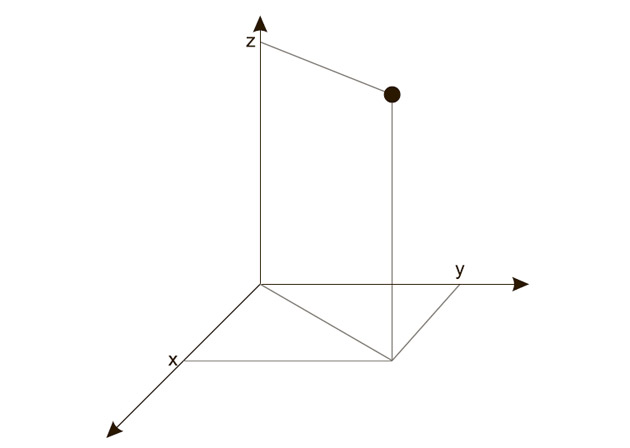
\includegraphics[width=0.5\linewidth]{Отчет (картинка 1).jpg}
    \caption{Положение точки в трехмерном пространстве}
    \label{fig:enter-label}
\end{figure}

Рассматривается задача восстановления вершин выпуклого многоугольника на фиксированной высоте $z$ по его опорной функции вращения $r(\alpha)$, заданной дискретно.

Опорная функция выпуклого многоугольника --- это расстояние от начала координат до опорной прямой с нормалью $e(\alpha)=(\cos\alpha,\sin\alpha)$, взятое в направлении нормали. Опорная прямая касается многоугольника в наиболее удаленной вершине, поэтому значение функции есть максимум проекций всех вершин:
\[
r(\alpha)=\max_{j=1,\dots,n}\left(x_j\cos\alpha+y_j\sin\alpha\right),
\]
где $(x_j,y_j)$ --- координаты вершин.

При фиксированном направлении величина $x\cos\alpha+y\sin\alpha$ есть проекция точки $(x,y)$ на это направление; именно такие проекции измеряются в задаче. Если $\alpha_i$ --- направление максимума, то вершина лежит на опорной прямой и восстанавливается по значению функции:
\[
x_i=r(\alpha_i)\cos\alpha_i,\qquad y_i=r(\alpha_i)\sin\alpha_i.
\]
В точке максимума производная $r'(\alpha)=-x\sin\alpha+y\cos\alpha$ обращается в нуль, откуда $x_i/\cos\alpha_i=y_i/\sin\alpha_i=r(\alpha_i)$ --- полезное соотношение для проверки. Требуется восстановить вершины по дискретно заданным значениям $r(\alpha_k)$.

\subsection{Основная идея метода}

Рассматривается функция $r(\alpha)$, заданная дискретно. Вершины многоугольника определяются как локальные максимумы этой функции.

\subsection{Определение максимума}

Для каждой точки $i$ вычисляются разности:
\[
d_1 = r_i - r_{i-1}, \quad d_2 = r_{i+1} - r_i.
\]

Точка считается локальным максимумом, если:
\[
d_1 \ge 0 \quad \text{и} \quad d_2 < 0.
\]

Для визуализации сгенерированных входных данных была написана программа $visualize.py$, для выходных – $reconstruct.py$. Ниже приведены результаты тестирования на точных данных.

\begin{figure}[H]
    \centering
    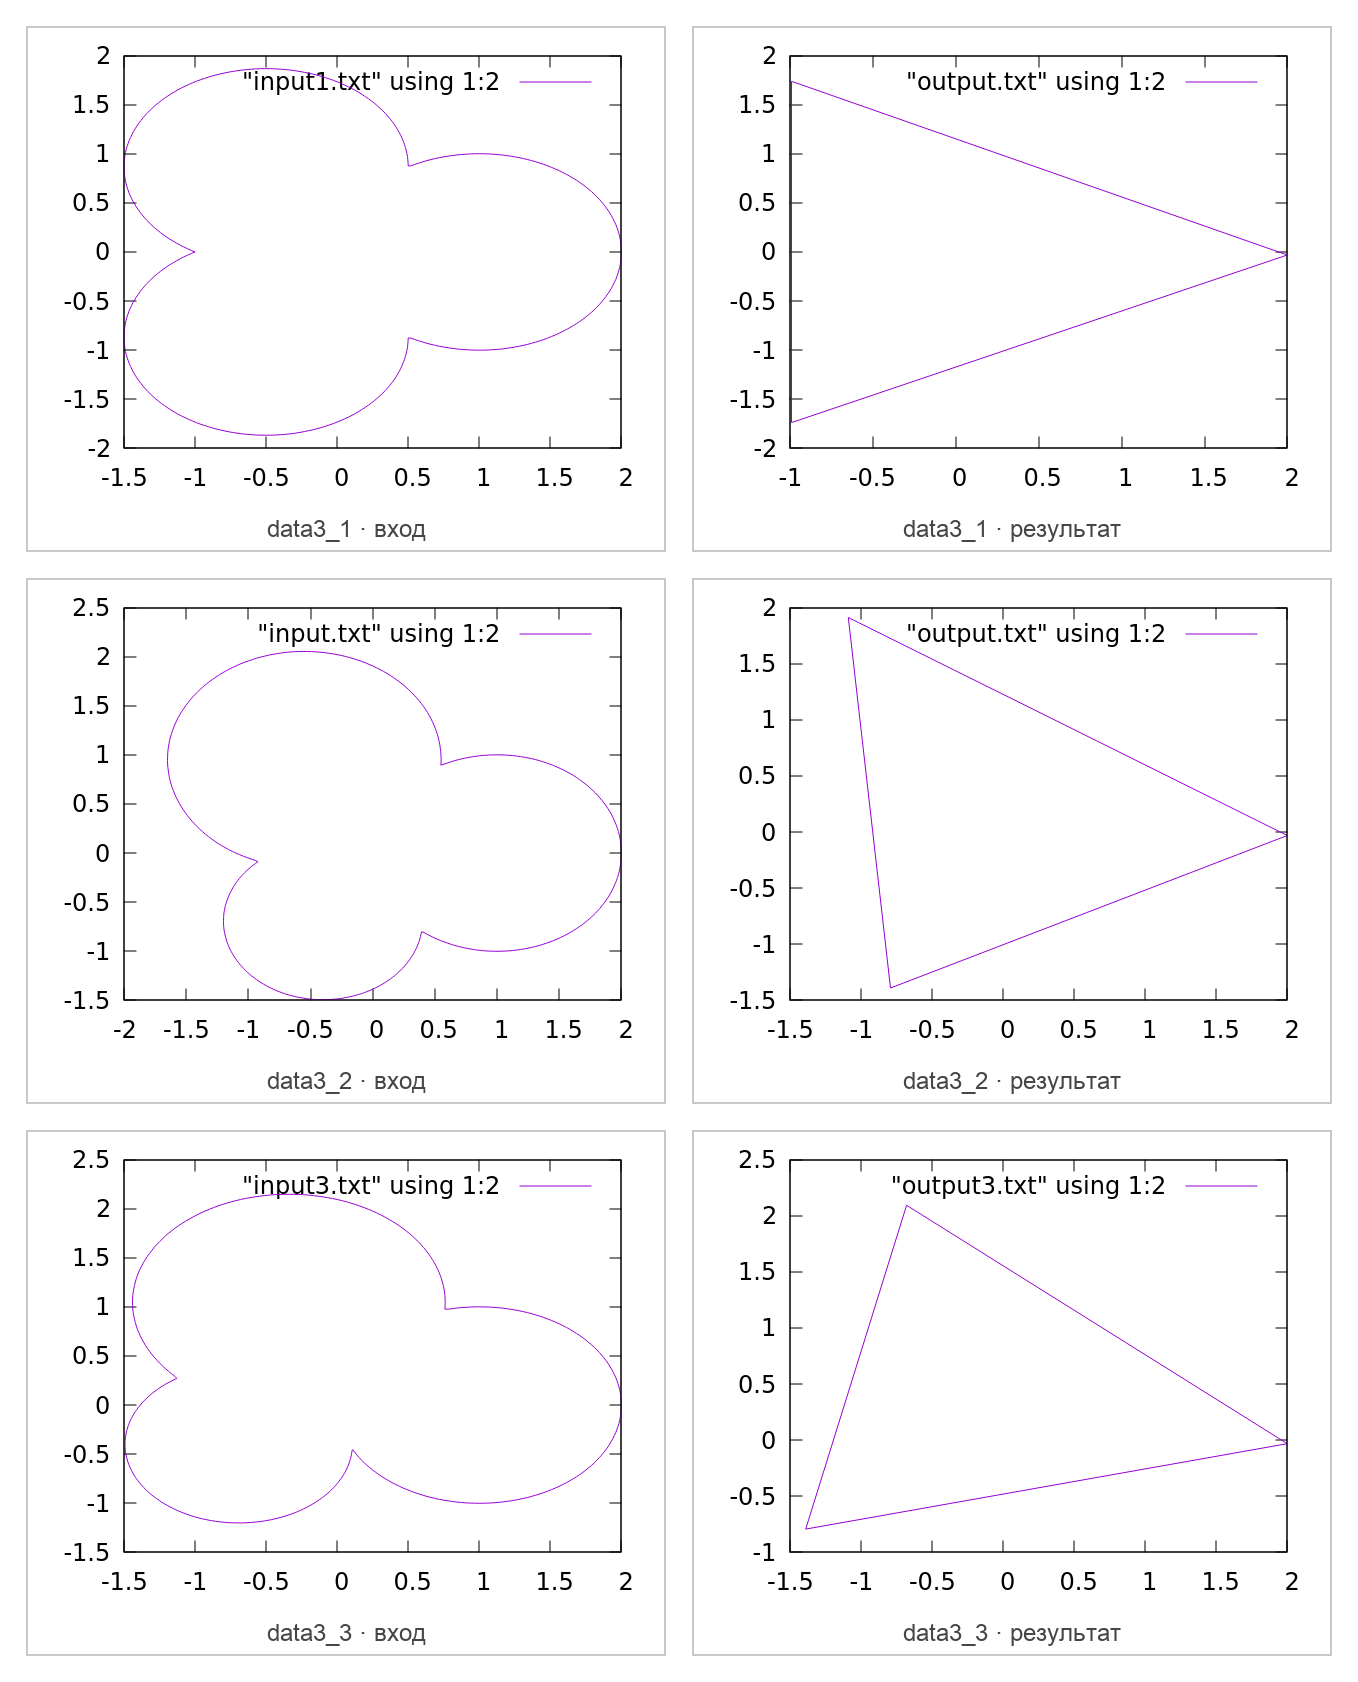
\includegraphics[width=0.95\linewidth]{fig2d_a.png}
    \caption{Точные данные data3\_1, data3\_2, data3\_3: слева входной контур, справа восстановленный многоугольник}
    \label{fig:2d_a}
\end{figure}

\begin{figure}[H]
    \centering
    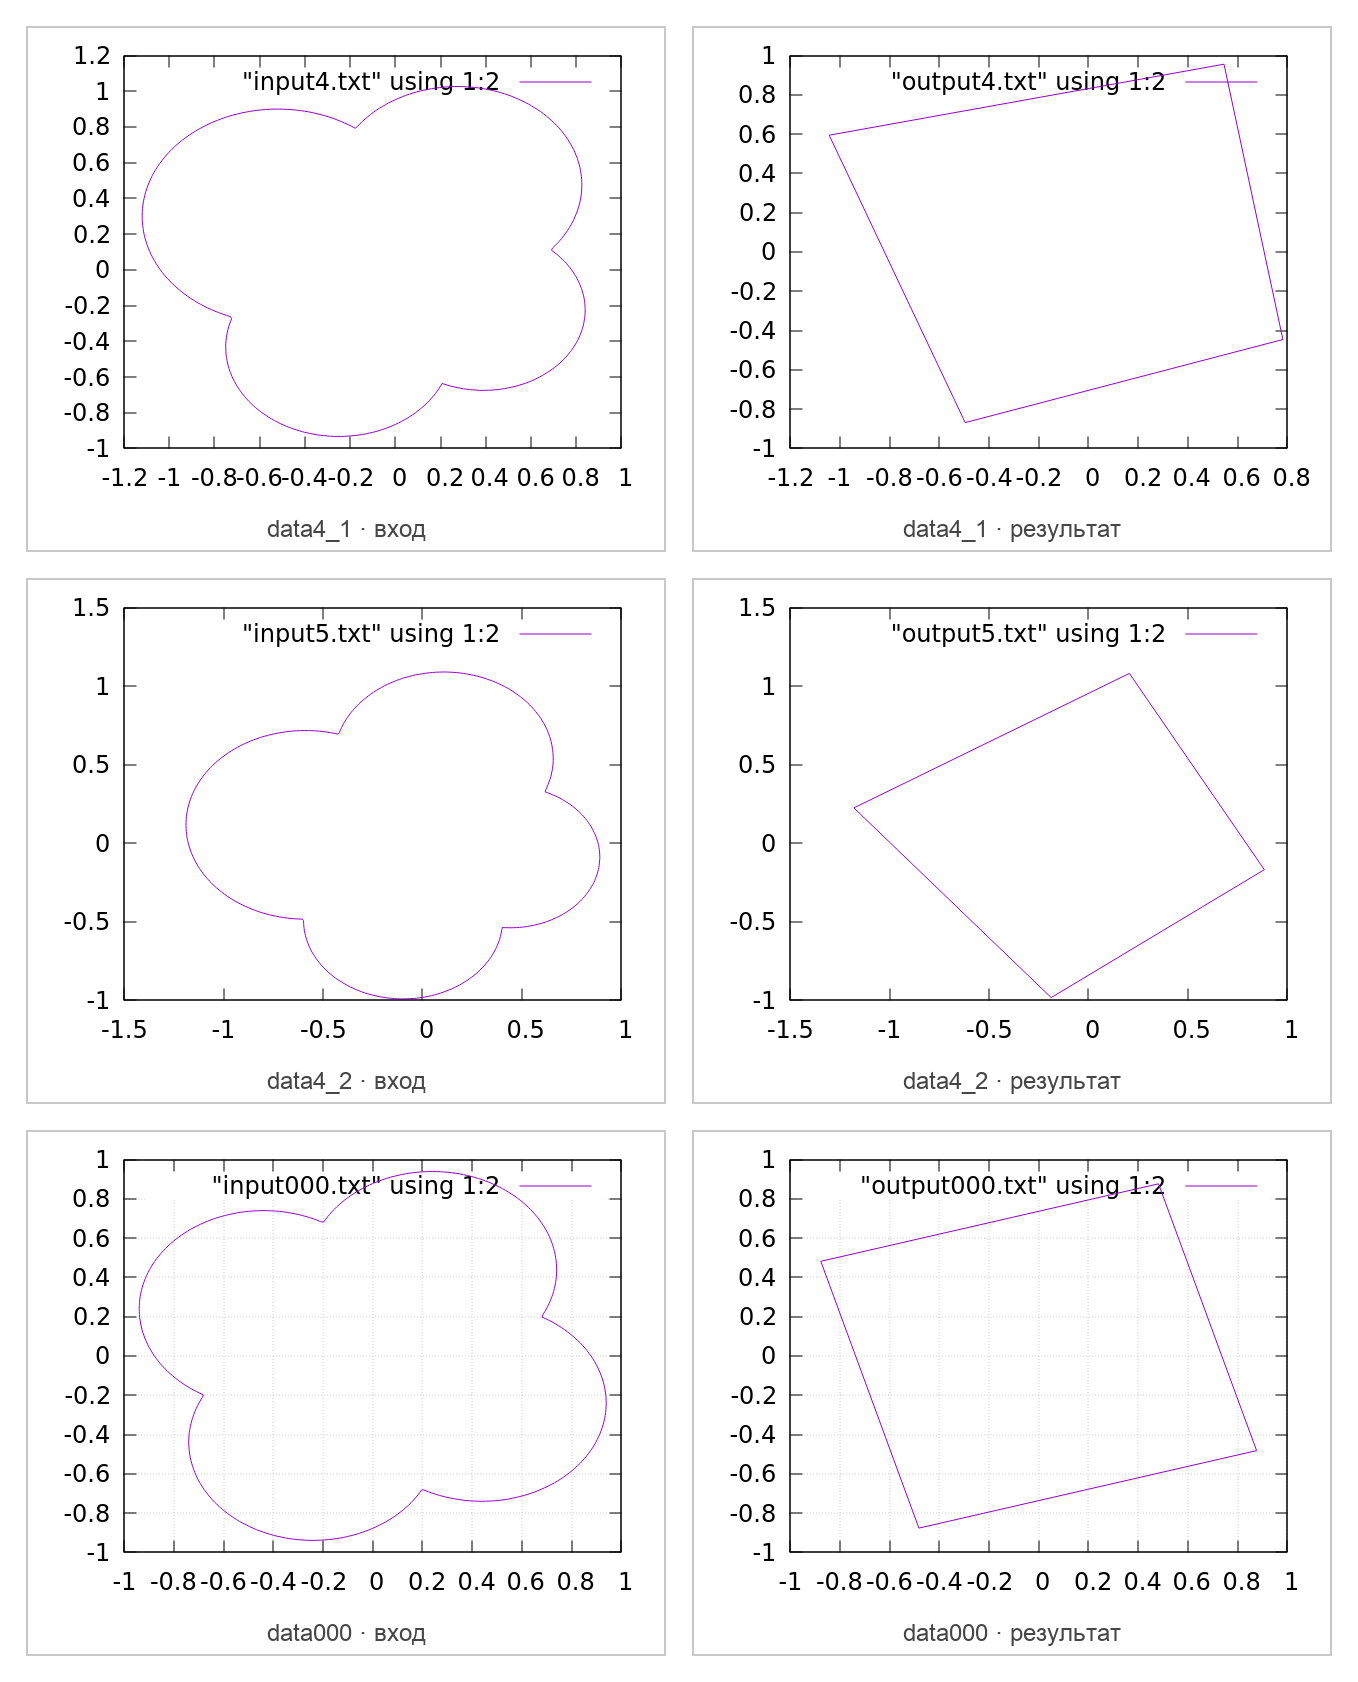
\includegraphics[width=0.95\linewidth]{fig2d_b.png}
    \caption{Точные данные data4\_1, data4\_2, data000: слева входной контур, справа восстановленный многоугольник}
    \label{fig:2d_b}
\end{figure}

Также протестировано на других данных ниже.

\begin{figure}[H]
    \centering
    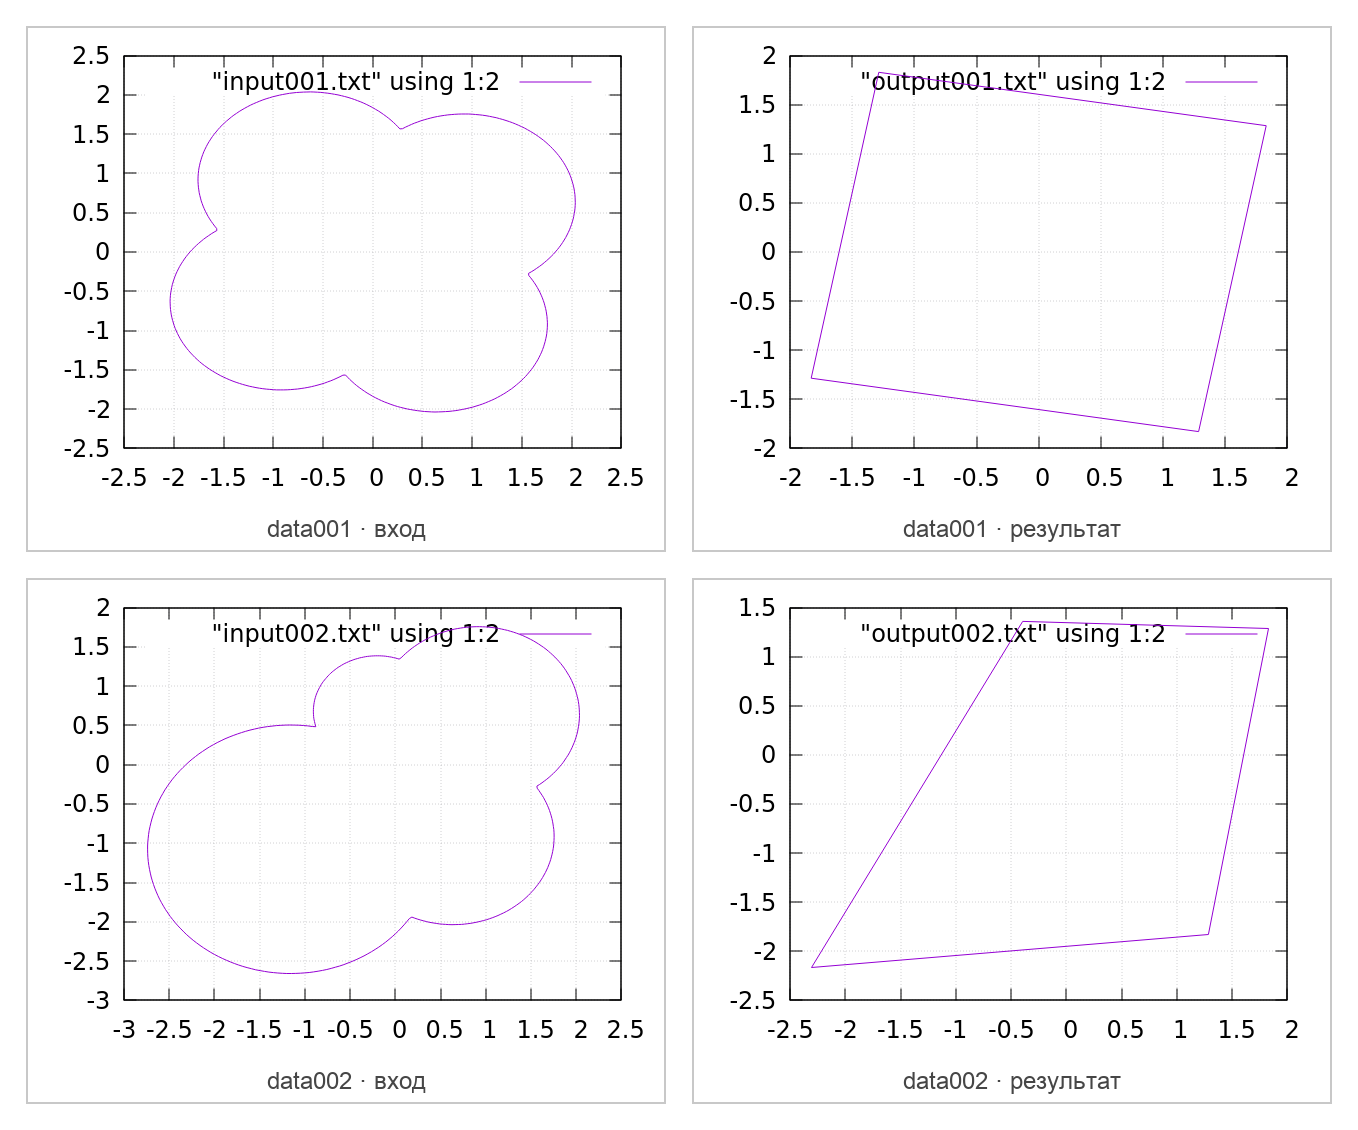
\includegraphics[width=0.95\linewidth]{fig2d_c.png}
    \caption{Точные данные data001, data002: слева входной контур, справа восстановленный многоугольник}
    \label{fig:2d_c}
\end{figure}

\begin{figure}[H]
    \centering
    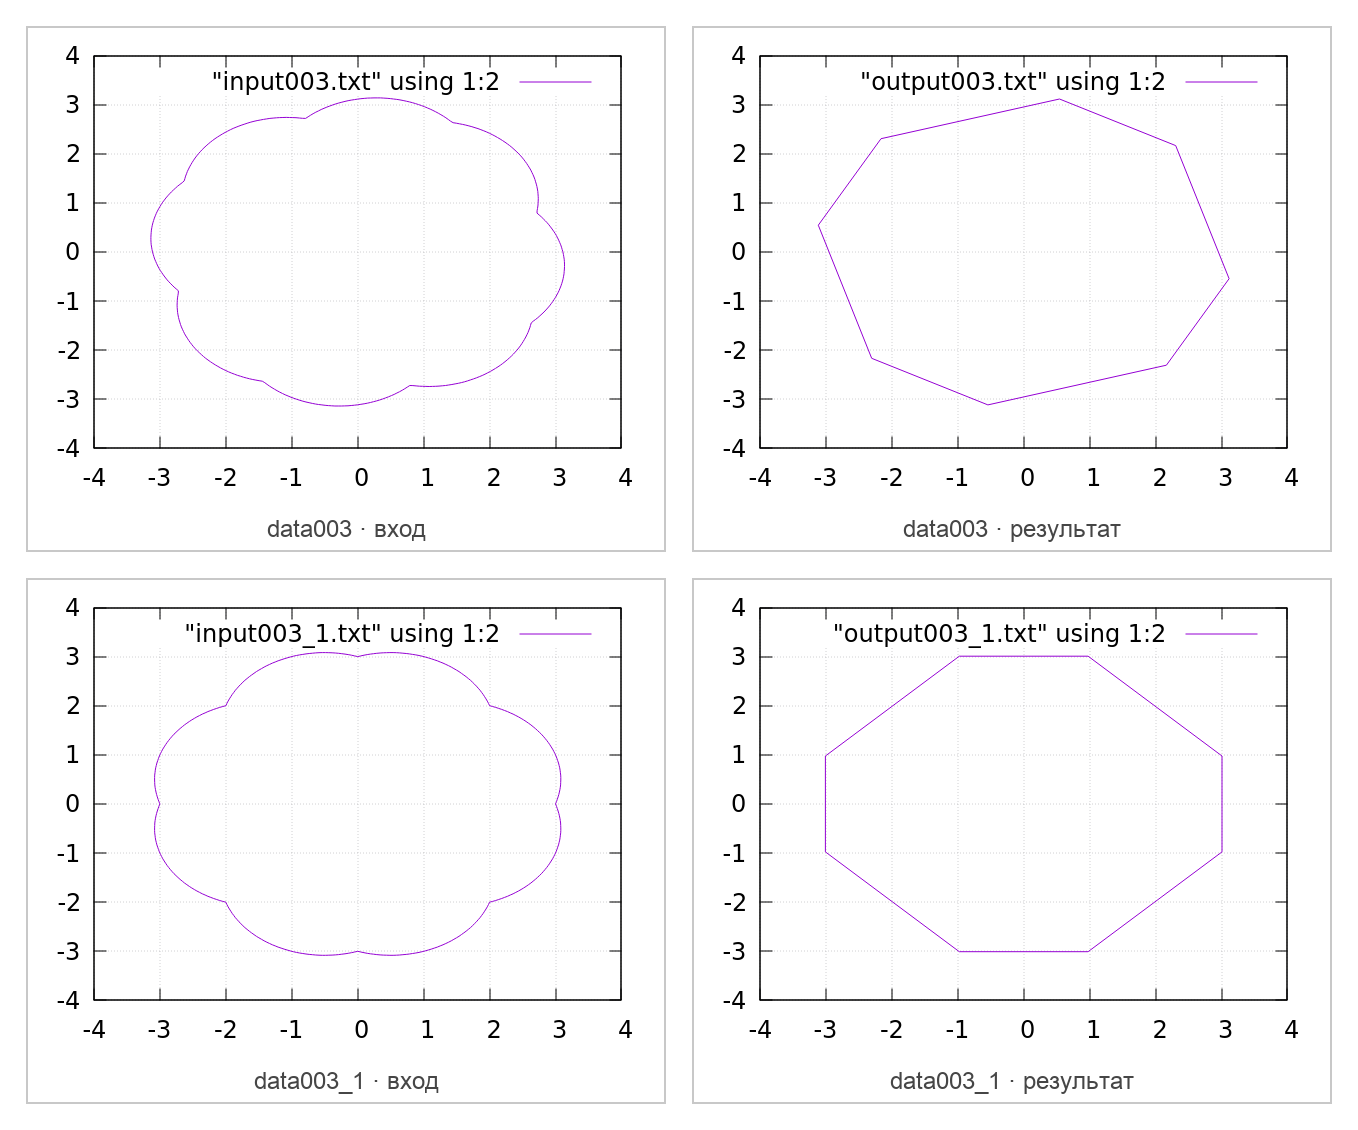
\includegraphics[width=0.95\linewidth]{fig2d_d.png}
    \caption{Точные данные data003, data003\_1: слева входной контур, справа восстановленный многоугольник}
    \label{fig:2d_d}
\end{figure}

\clearpage
\section{Генерация горизонтальных контуров и моделирование шума}

Для тестирования алгоритмов восстановления формы объекта использовалась процедура генерации горизонтальных контуров выпуклого многоугольника.

\subsection{Исходная модель}

Исходный контур задаётся набором вершин:
\[
P_k = (x_k, y_k).
\]

В программе для генерации data003\_1.txt использовался восьмиугольник:
\[
(3,1),\ (1,3),\ (-1,3),\ (-3,1),\ (-3,-1),\ (-1,-3),\ (1,-3),\ (3,-1).
\]

\subsection{Формирование проекций}

Для каждого направления проекции вычисляется расстояние от начала координат до опорной прямой.

Угол проекции определяется как:
\[
\alpha_i = i h,
\]
где
\[
h = \frac{2\pi}{n},
\]
а $n$ — число проекций.

Для каждой вершины вычисляется:
\[
r = \sqrt{x^2 + y^2},
\]
\[
\varphi = \arctan2(y,x).
\]

Затем для каждого угла проекции определяется значение:
\[
p_i = r \cos(\alpha_i + \varphi).
\]

Данная величина представляет собой проекцию вершины на направление наблюдения.

\subsection{Построение горизонтального контура}

Контур формируется как максимум среди проекций всех вершин:
\[
R(\alpha_i) = \max_k p_i^{(k)}.
\]

Таким образом, для каждого угла выбирается наиболее удалённая точка силуэта.

Полученная функция:
\[
R(\alpha)
\]
является дискретной опорной функцией выпуклого многоугольника.

\subsection{Моделирование шума}

Для имитации ошибок измерения в проекции добавляется случайный шум:
\[
\widetilde{p_i} = p_i + \varepsilon,
\]
где
\[
\varepsilon = r_v \cdot \xi,
\]
\[
\xi \in [-1,1].
\]

Параметр:
\[
r_v
\]
задаёт амплитуду шума.

В работе использовались значения (в названиях файлов далее r8 и r80 соответственно):
\[
r_v = 0.008,\ 0.08.
\]

Шум моделирует:
\begin{itemize}
    \item ошибки измерений,
    \item дискретизацию,
    \item неточности восстановления контуров.
\end{itemize}

\subsection{Результат генерации}

В результате формируется набор данных:
\[
(\alpha_i,\ R(\alpha_i)),
\]
который записывается в текстовый файл и далее используется для восстановления геометрии объекта.

\clearpage
\section{Подавление шума методом наименьших квадратов}

Для уменьшения влияния шума использовалась аппроксимация опорной функции при помощи ряда Фурье и метода наименьших квадратов, а также вспомогательного метода "ближайших соседей"\ (взвешенного скользящего среднего).

\subsection{Исходные данные}

После генерации контуров формируется набор значений:
\[
(\alpha_i, r_i),
\]
где:
\begin{itemize}
    \item $\alpha_i$ — угол проекции,
    \item $r_i$ — расстояние до опорной прямой.
\end{itemize}

Из-за добавления случайного шума значения содержат ошибки:
\[
r_i = r_i^{\text{true}} + \varepsilon_i.
\]

\subsection{Аппроксимация рядом Фурье}

Поскольку функция:
\[
r(\alpha)
\]
является периодической, она представляется рядом Фурье:
\[
r(\alpha) \approx
a_0 +
\sum_{k=1}^{m}
\left(
a_k \cos(k\alpha)
+
b_k \sin(k\alpha)
\right),
\]
где:
\begin{itemize}
    \item $m$ — число гармоник,
    \item $a_k$, $b_k$ — коэффициенты разложения.
\end{itemize}

\subsection{Метод наименьших квадратов}

Для вычисления коэффициентов строится система:
\[
A c \approx r,
\]
где:
\[
A =
\begin{bmatrix}
1 & \cos(\alpha_1) & \sin(\alpha_1) & \dots \\
1 & \cos(\alpha_2) & \sin(\alpha_2) & \dots \\
\vdots & \vdots & \vdots & \ddots
\end{bmatrix},
\]
\[
c =
\begin{bmatrix}
a_0 & a_1 & b_1 & \dots
\end{bmatrix}^T.
\]

Коэффициенты определяются из условия минимизации квадратичной ошибки:
\[
\|Ac-r\|^2 \rightarrow \min.
\]

Решение вычисляется методом наименьших квадратов:
\[
c = (A^T A)^{-1} A^T r.
\]

\subsection{Метод «ближайших соседей»}

Другой вспомогательный метод, который может дать лучшие приближения (ниже число итераций $k$ -- количество последовательных усреднений):

\[
\widetilde r(\alpha_i) = \frac{2r(\alpha_{i})+r(\alpha_{i-1})+r(\alpha_{i+1})}{4}.
\]

Для данного метода была написана программа $denoise\_uniform.py$ с автоматической регулировкой числа $k$ итераций усреднения при сравнении с эталоном (для сглаживания был установлен нижний порог $k$ = 5):

\[
\mathrm{RMSE}(k)
=
\sqrt{
\frac{1}{n}
\sum_{i=1}^{n}
\left(
r_i - \widetilde r_i^{(k)}
\right)^2
}
\]

\[
k_{\mathrm{opt}} =
\operatorname*{arg\,min}_{k} \mathrm{RMSE}(k)
\]

\subsection{Результат и сравнение с точной формой}

После вычисления коэффициентов получается сглаженная функция:
\[
\widetilde r(\alpha),
\]
которая приближает исходную форму объекта и подавляет высокочастотный шум. Для этого была написана программа $denoise.py$.

Полученные данные далее используются для восстановления геометрии многоугольника.

\clearpage
\section{Сравнение восстановленной и точной формы}

Для оценки качества восстановления выполнялось сравнение координат восстановленных точек с координатами точной модели.

Для каждой пары точек вычислялось евклидово расстояние:
\[
d_i =
\sqrt{
(x_i - \hat{x}_i)^2 +
(y_i - \hat{y}_i)^2
},
\]
где:
\begin{itemize}
    \item $(x_i,y_i)$ — точка точной модели,
    \item $(\hat{x}_i,\hat{y}_i)$ — восстановленная точка.
\end{itemize}

Качество восстановления оценивалось двумя величинами.

Среднеквадратичная ошибка:
\[
\mathrm{MSE}
=
\frac{1}{N}
\sum_{i=1}^{N} d_i^2.
\]

Максимальное отклонение:
\[
d_{\max} = \max_i d_i.
\]

Полученные значения позволяют оценить точность восстановления формы после подавления шума. Для этого была написана программа $compare.py$.

Ниже результаты тестирования на восьмиугольнике, параметр шума в названии файла. Также результаты тестирования в 3D, где сечения взяты на разных высотах.

\begin{figure}[H]
    \centering
    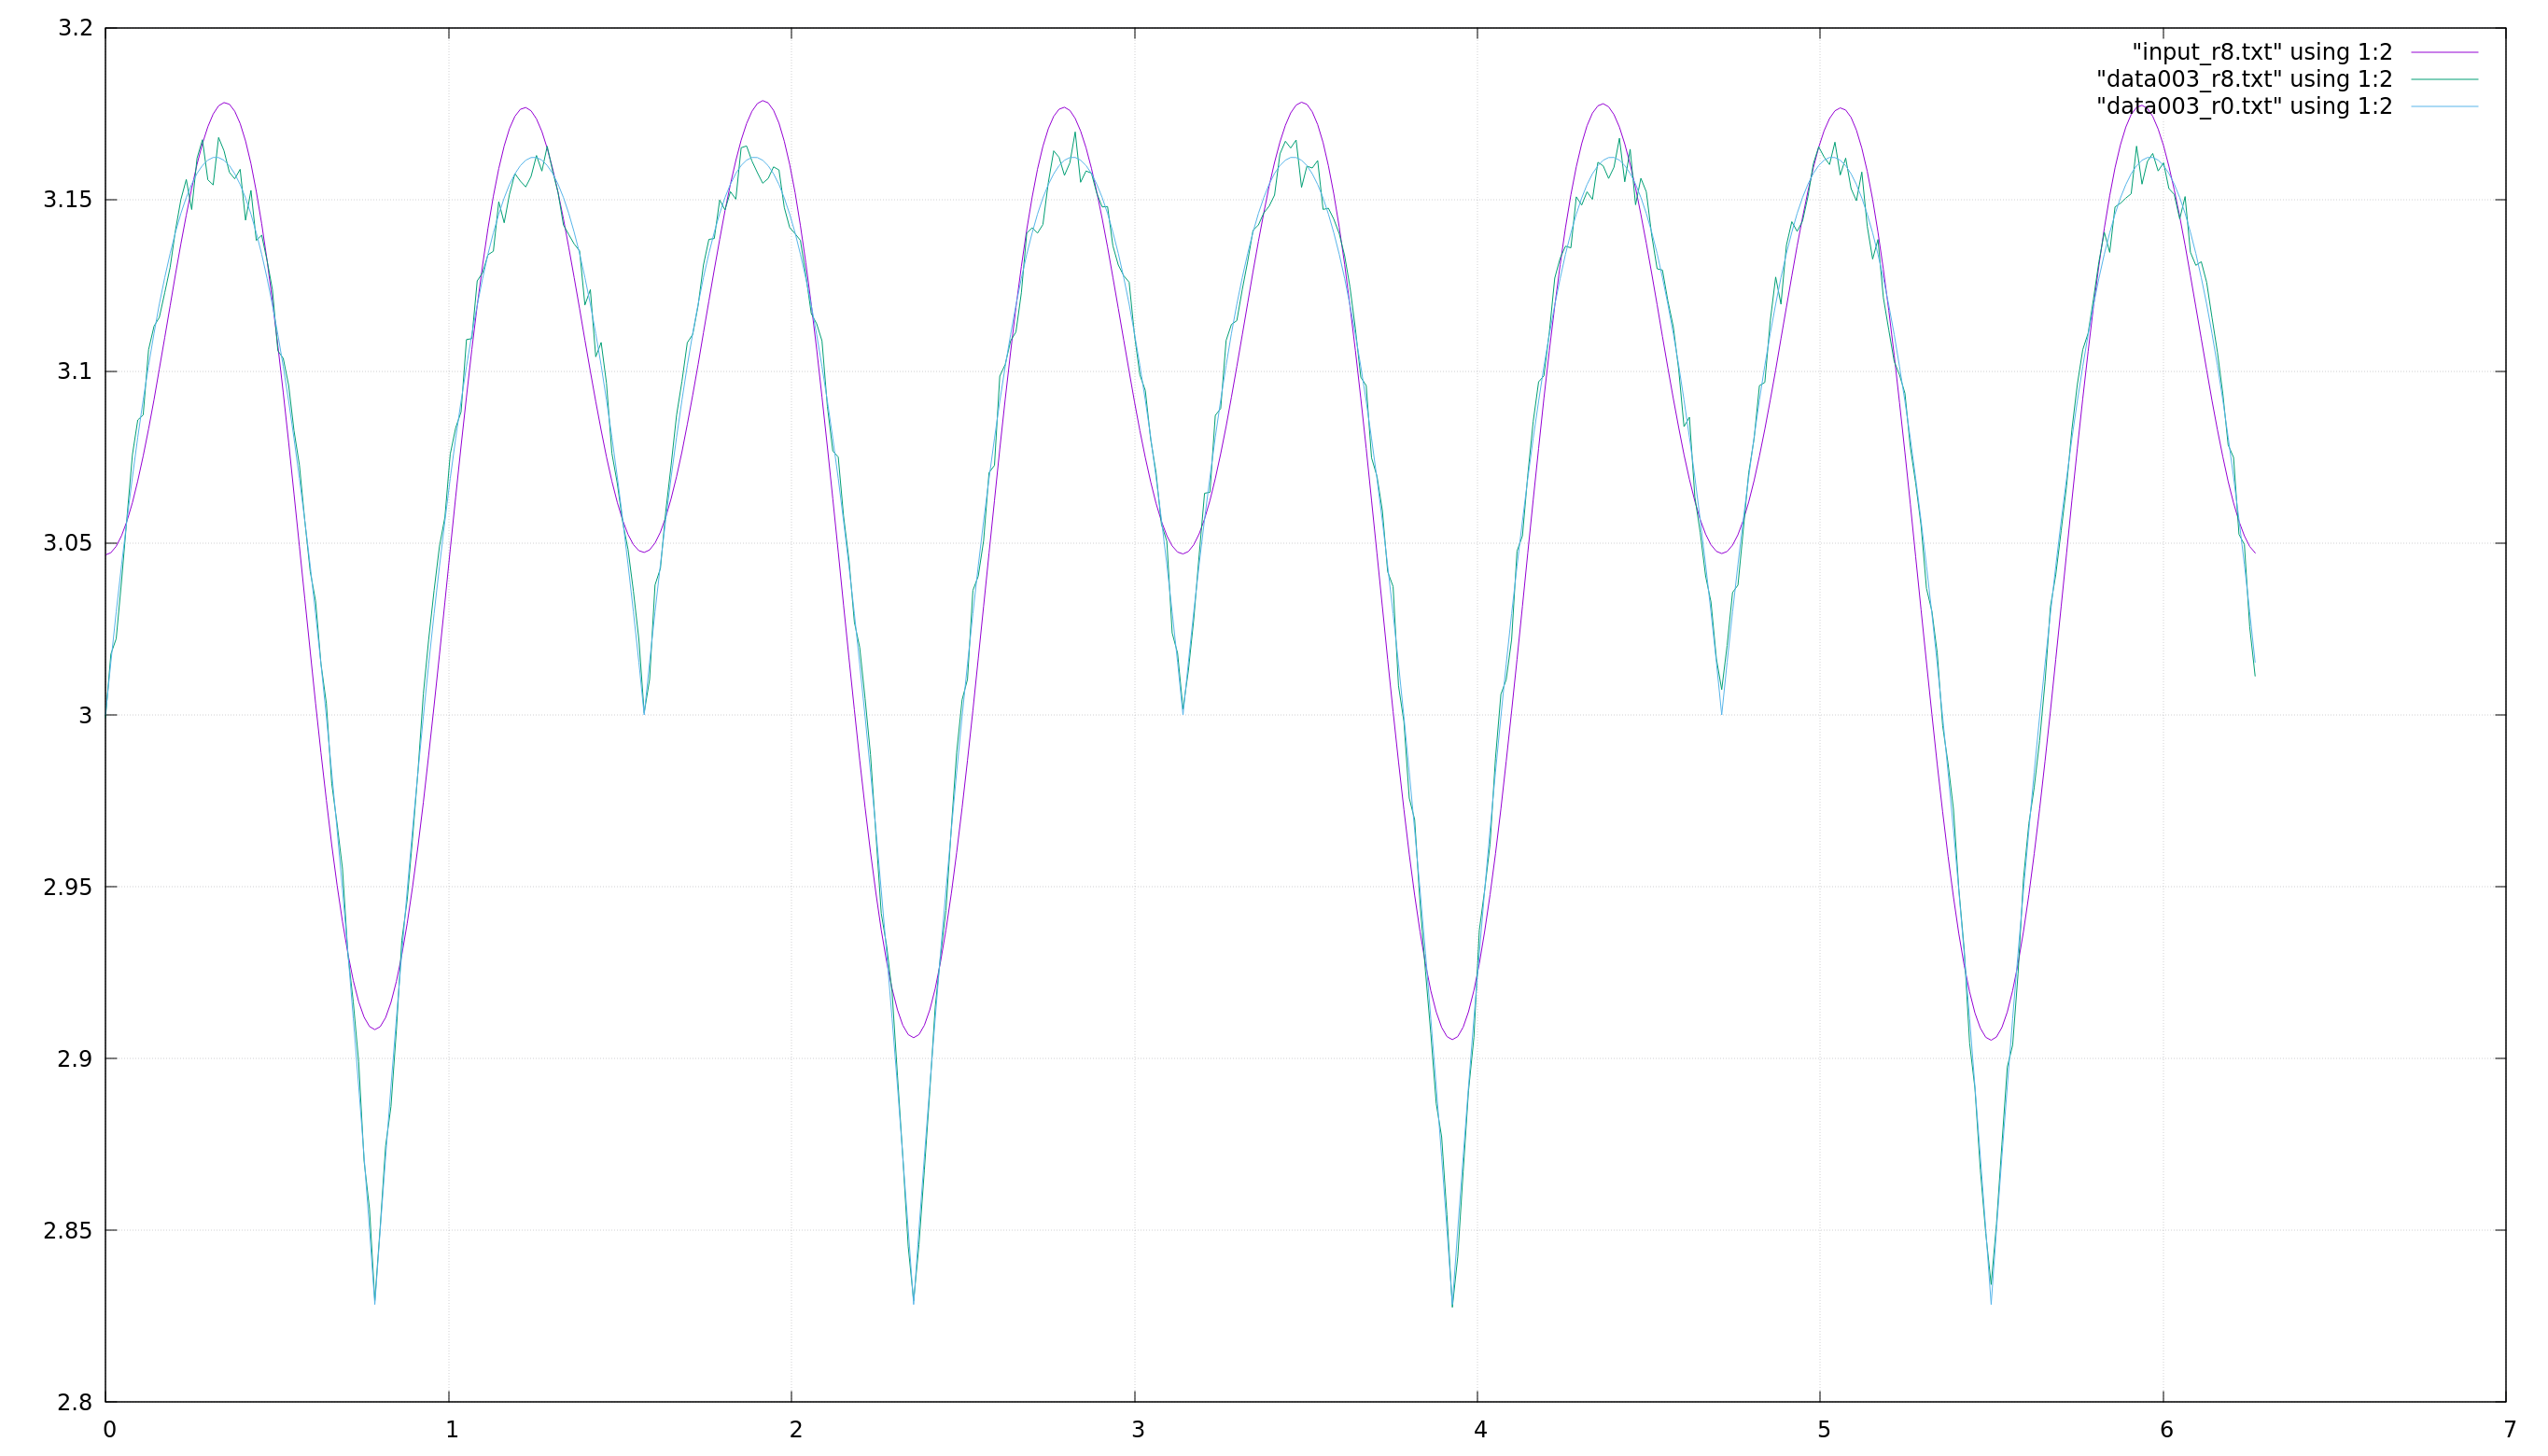
\includegraphics[width=0.8\linewidth]{input_r8_compare.png}
    \caption{Сравнение зашумленного и сглаженного варианта $r(\alpha)$ с эталоном}
\end{figure}

\begin{figure}[H]
    \centering
    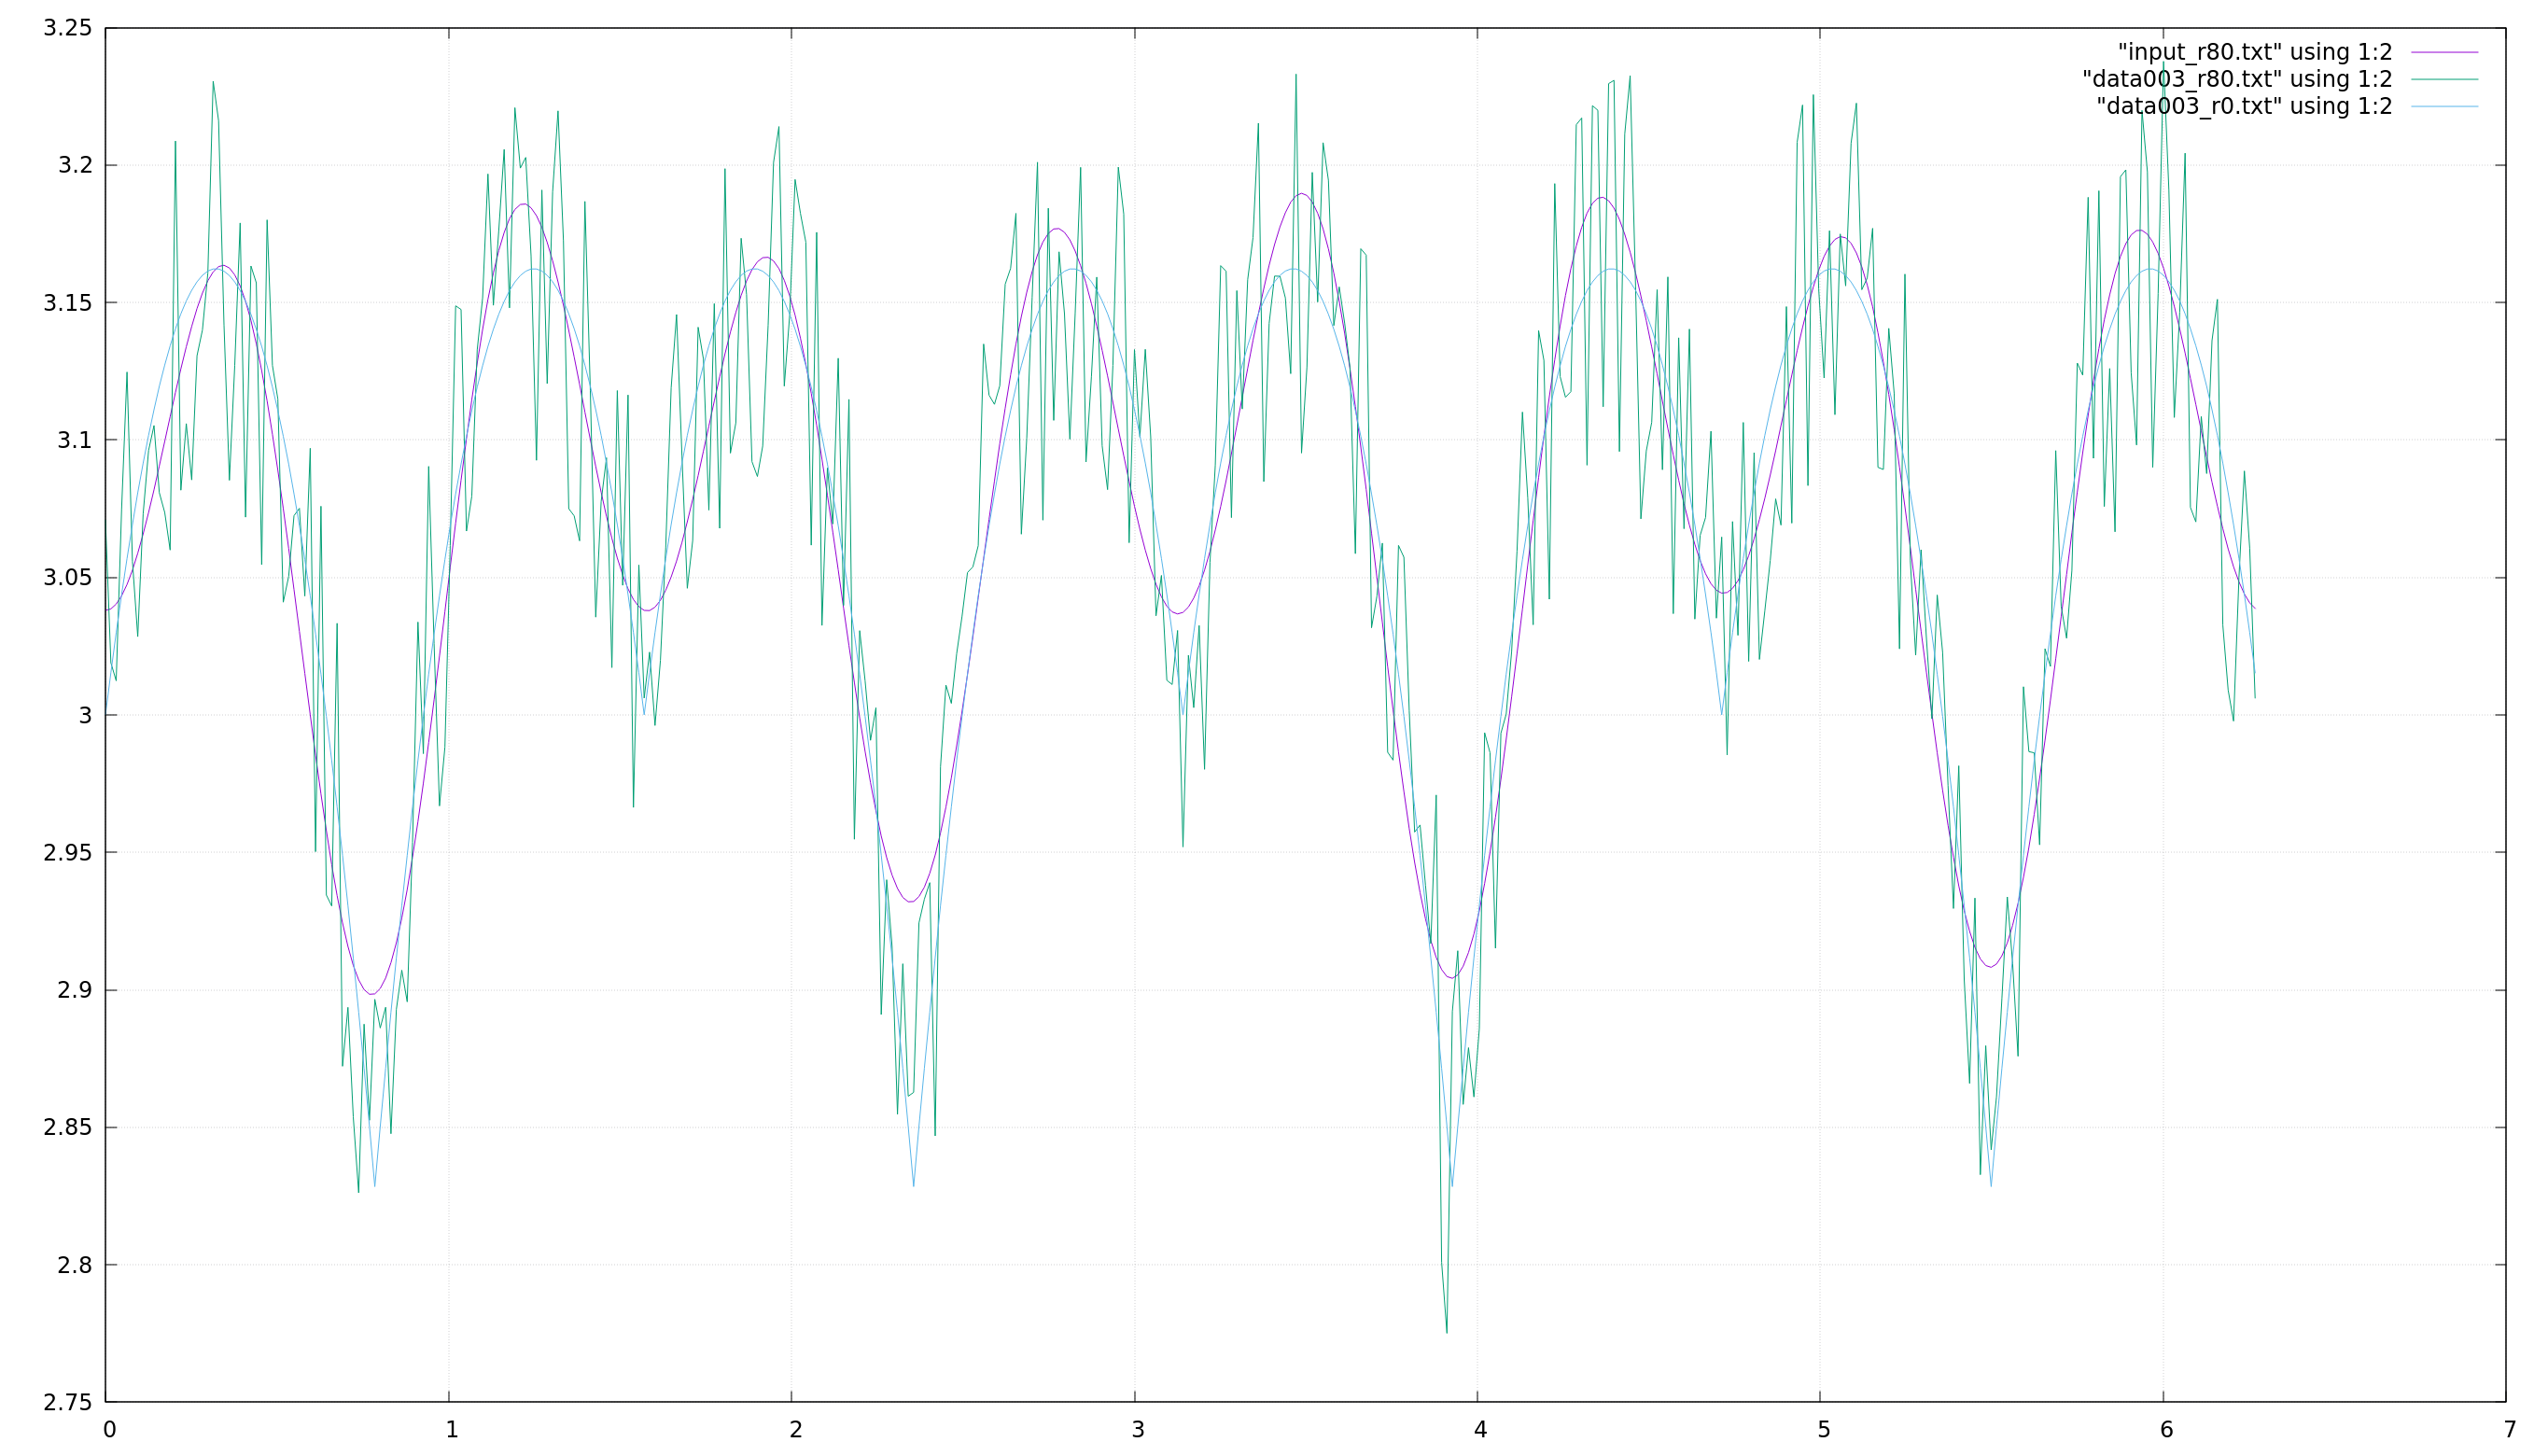
\includegraphics[width=0.8\linewidth]{input_r80_compare.png}
    \caption{Сравнение сильно зашумленного и сглаженного варианта $r(\alpha)$ с эталоном}
\end{figure}

\begin{figure}[H]
    \centering
    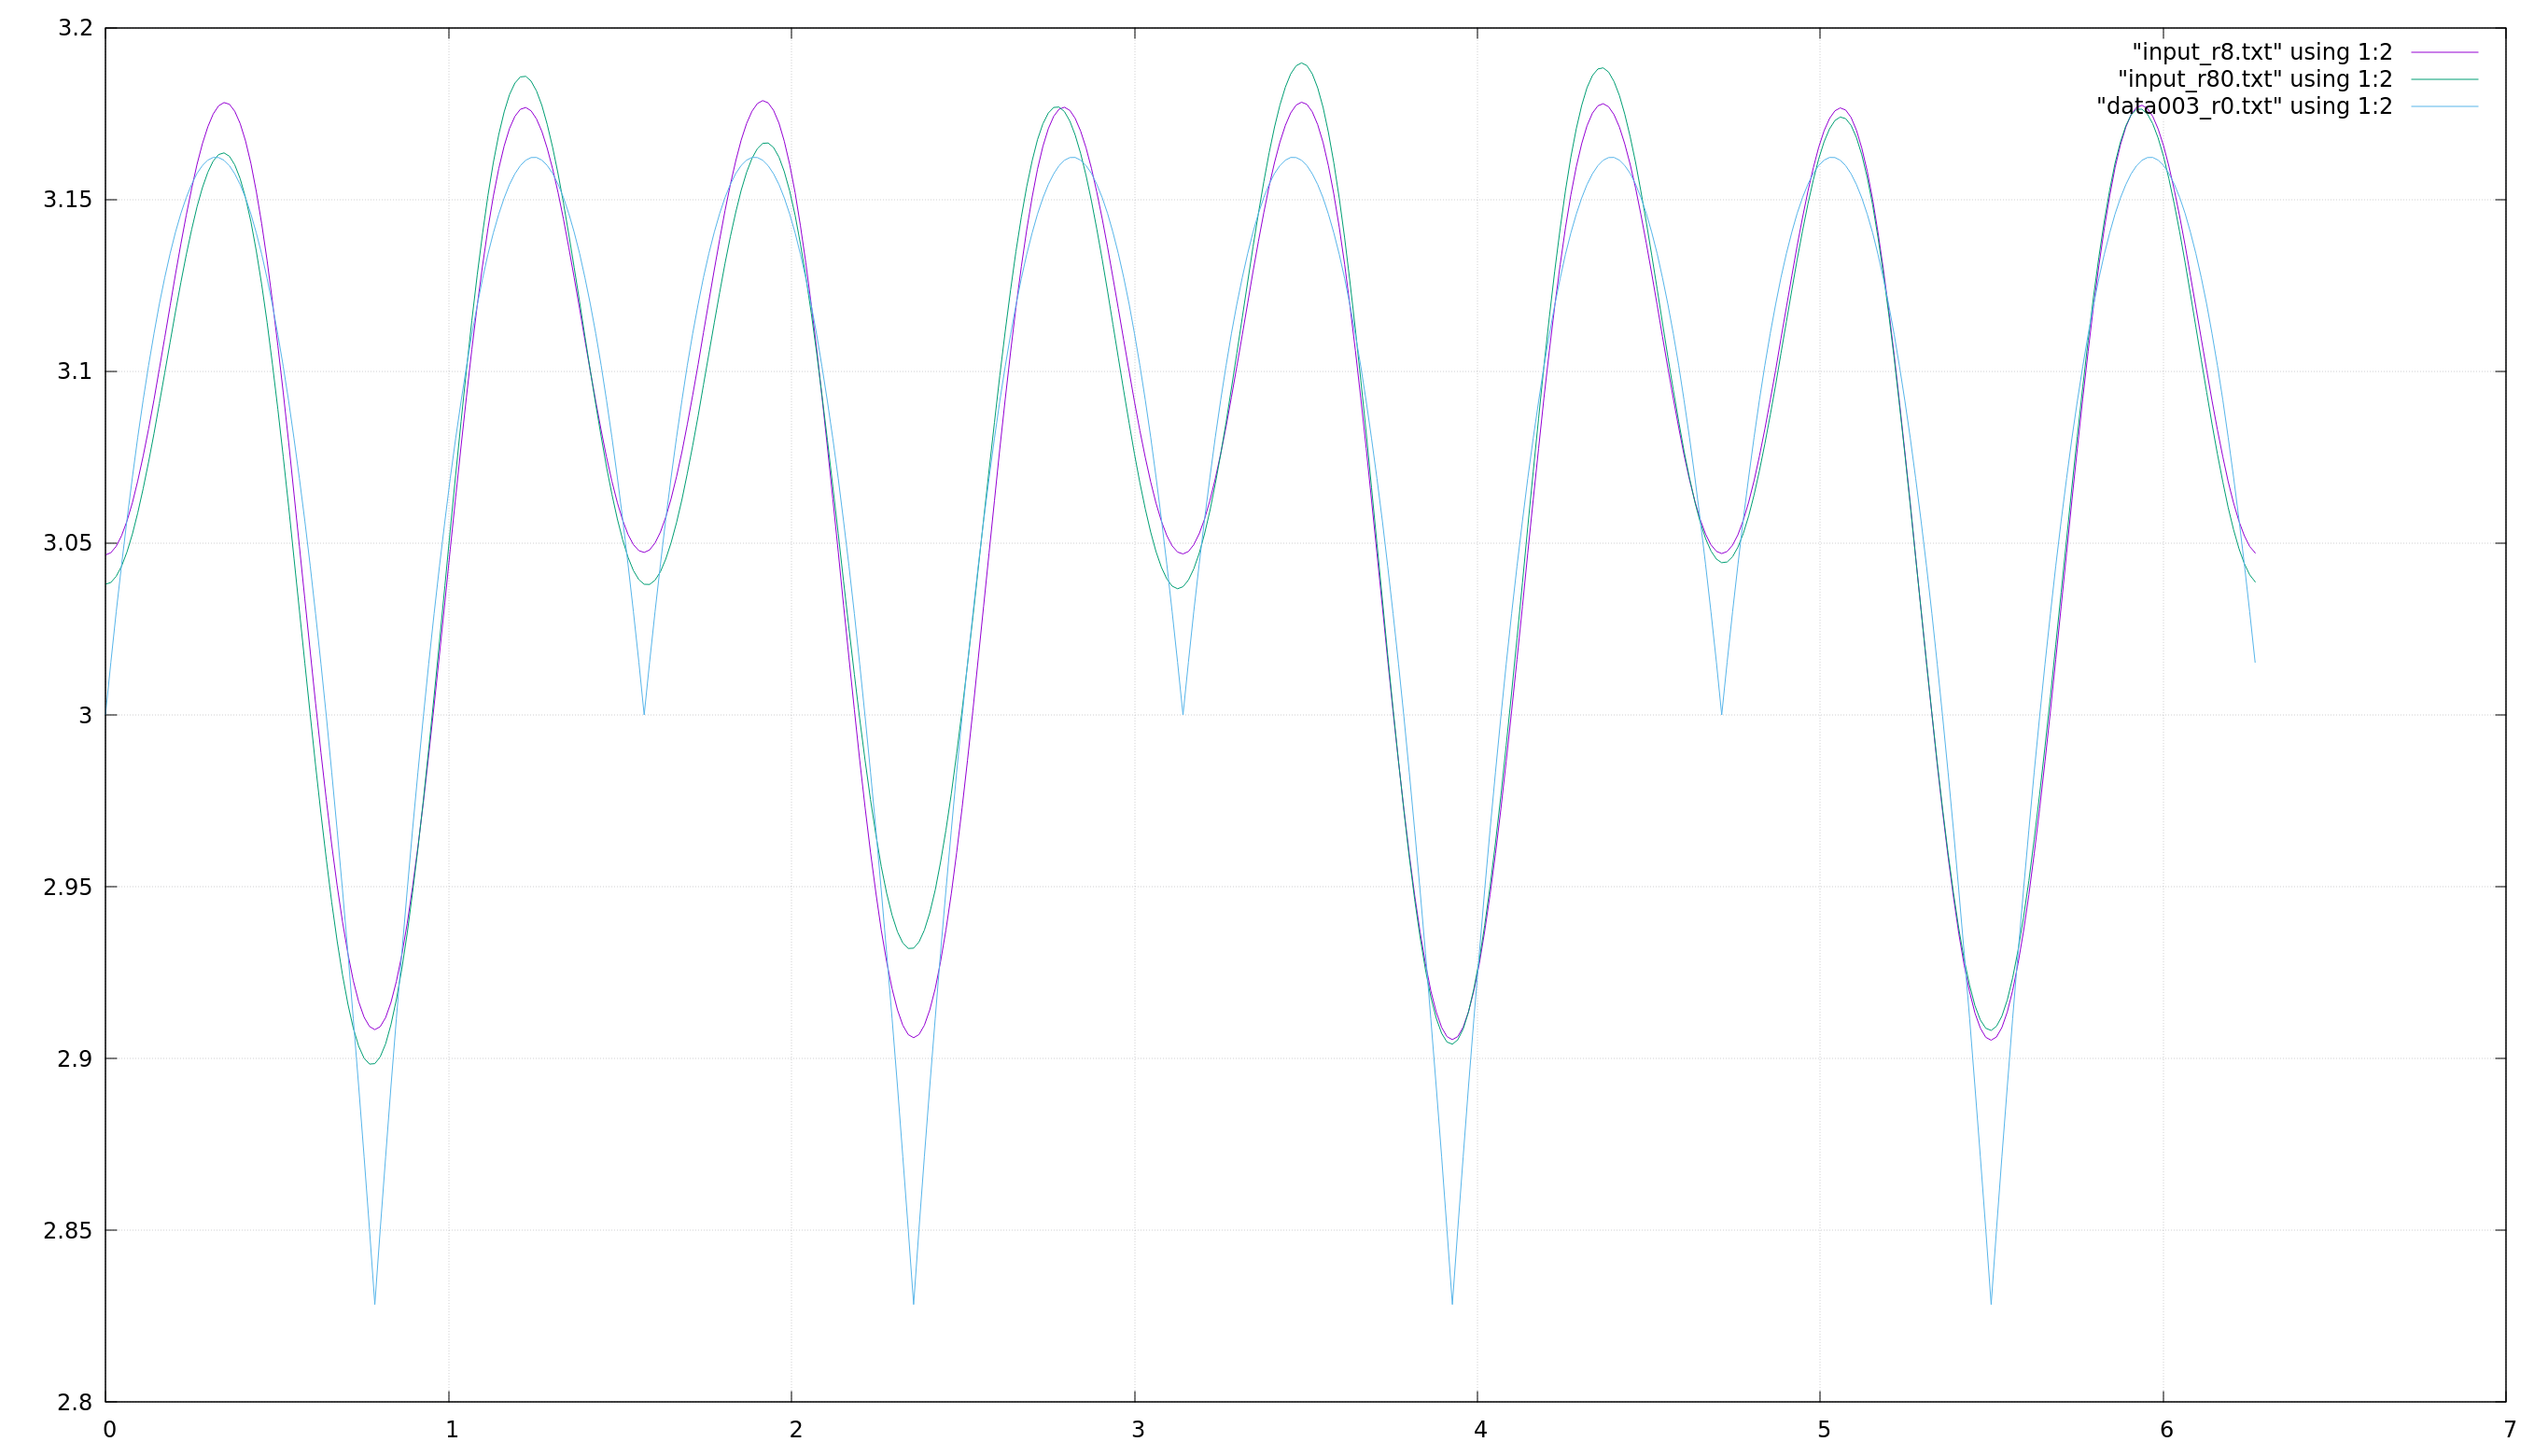
\includegraphics[width=0.8\linewidth]{input_compare.png}
    \caption{Сравнение сглаженных результатов с эталоном}
\end{figure}

\begin{figure}[H]
    \centering
    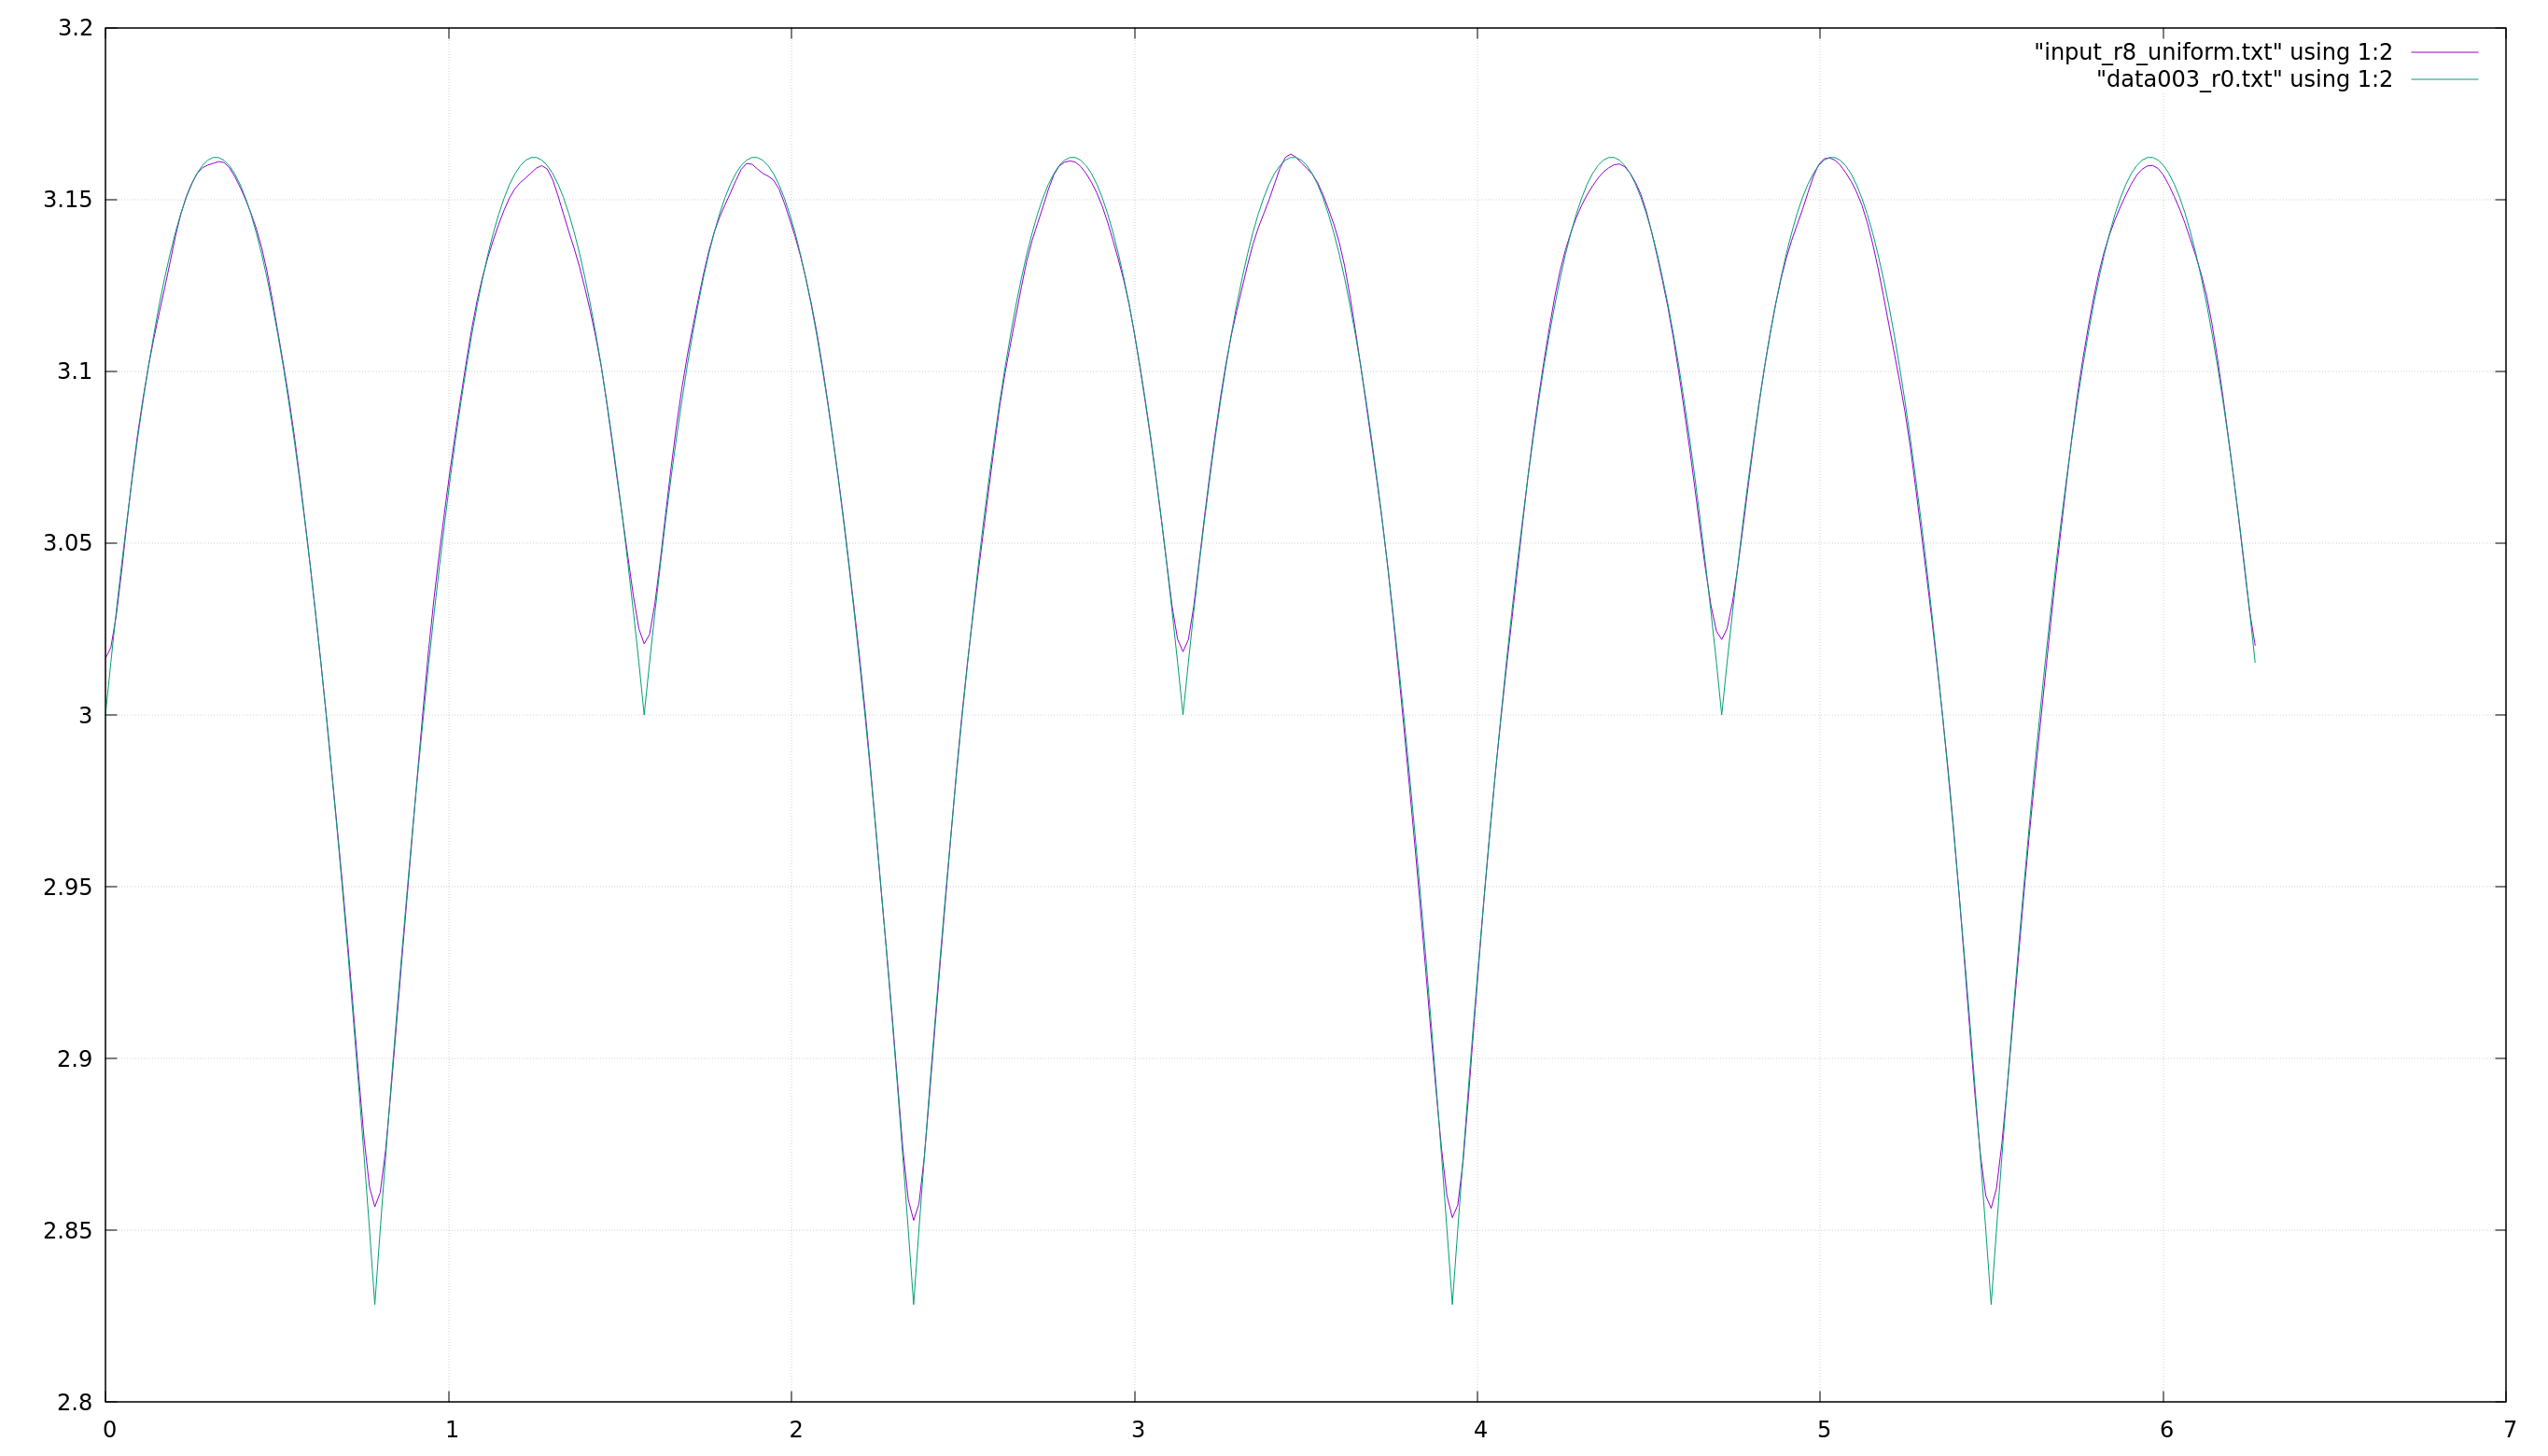
\includegraphics[width=0.8\linewidth]{input_r8_uniform_compare.png}
    \caption{Метод "ближайших соседей"\ для r8 ($k$ = 5)}
\end{figure}

\begin{figure}[H]
    \centering
    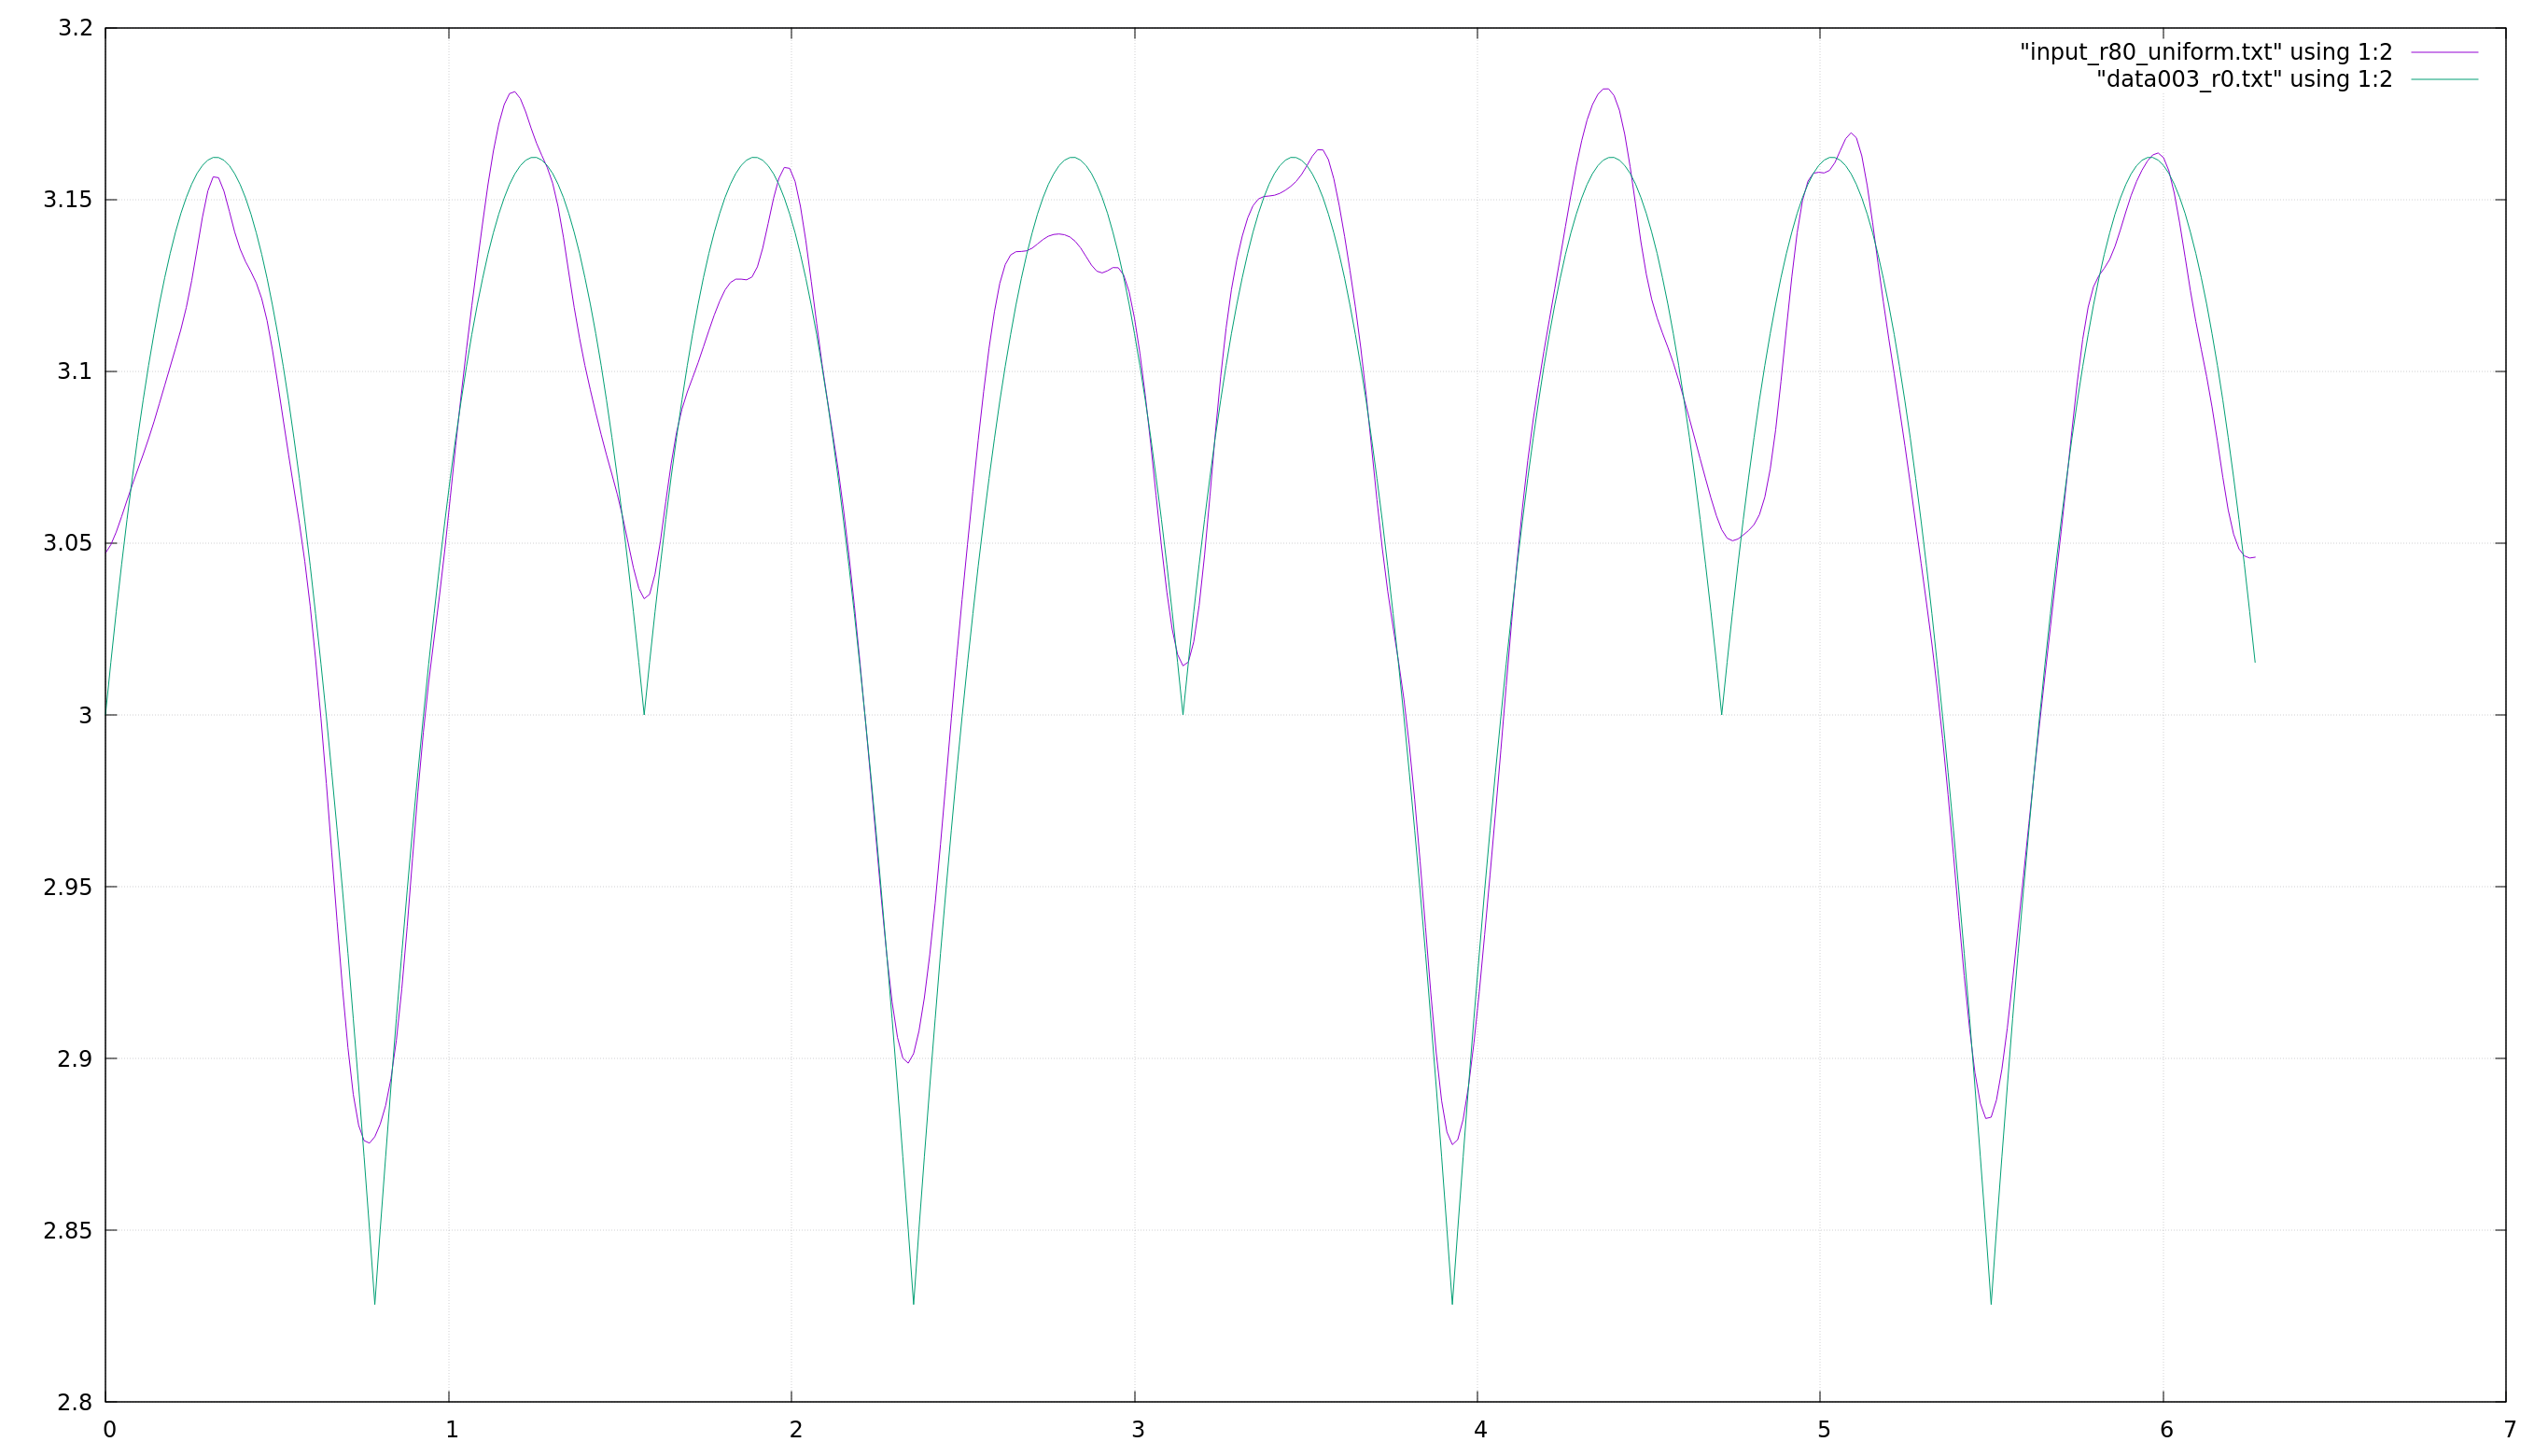
\includegraphics[width=0.8\linewidth]{input_r80_uniform_compare.png}
    \caption{Метод "ближайших соседей"\ для r80 ($k$ = 15)}
\end{figure}

\begin{figure}[H]
    \centering
    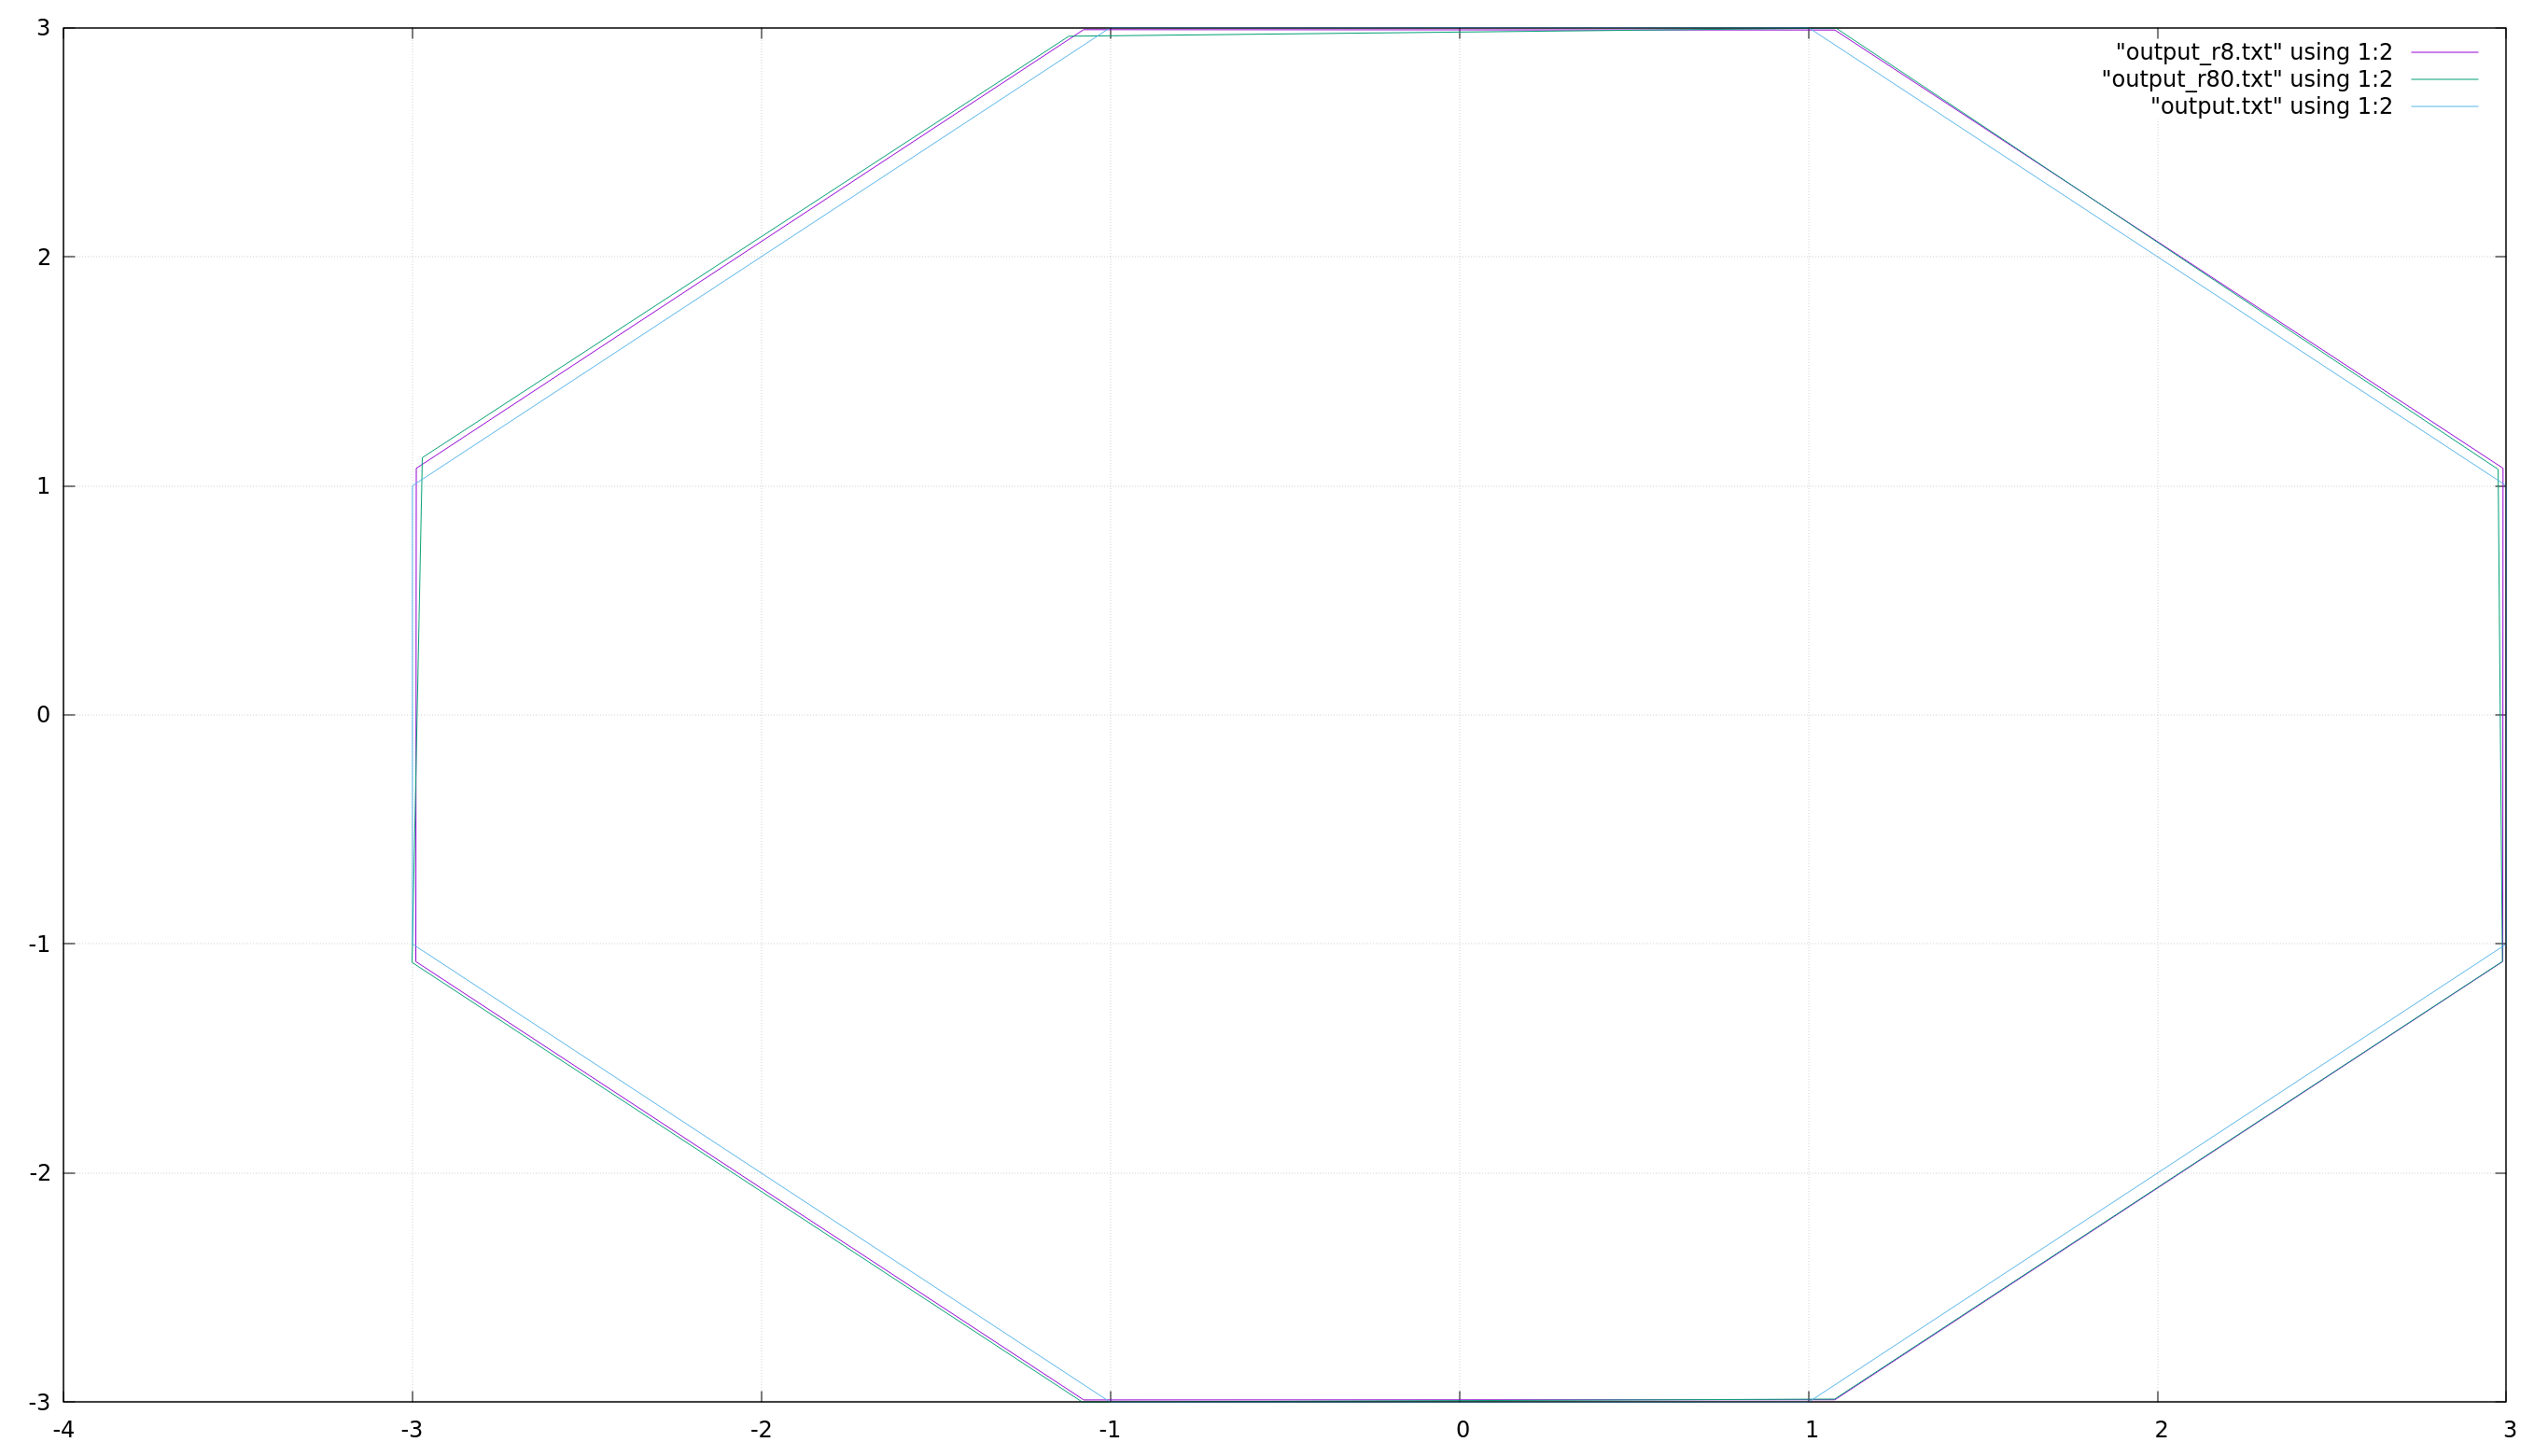
\includegraphics[width=0.8\linewidth]{output_compare.png}
    \caption{Сравнение восстановленных многоугольников с эталоном}
\end{figure}

\begin{figure}[H]
    \centering
    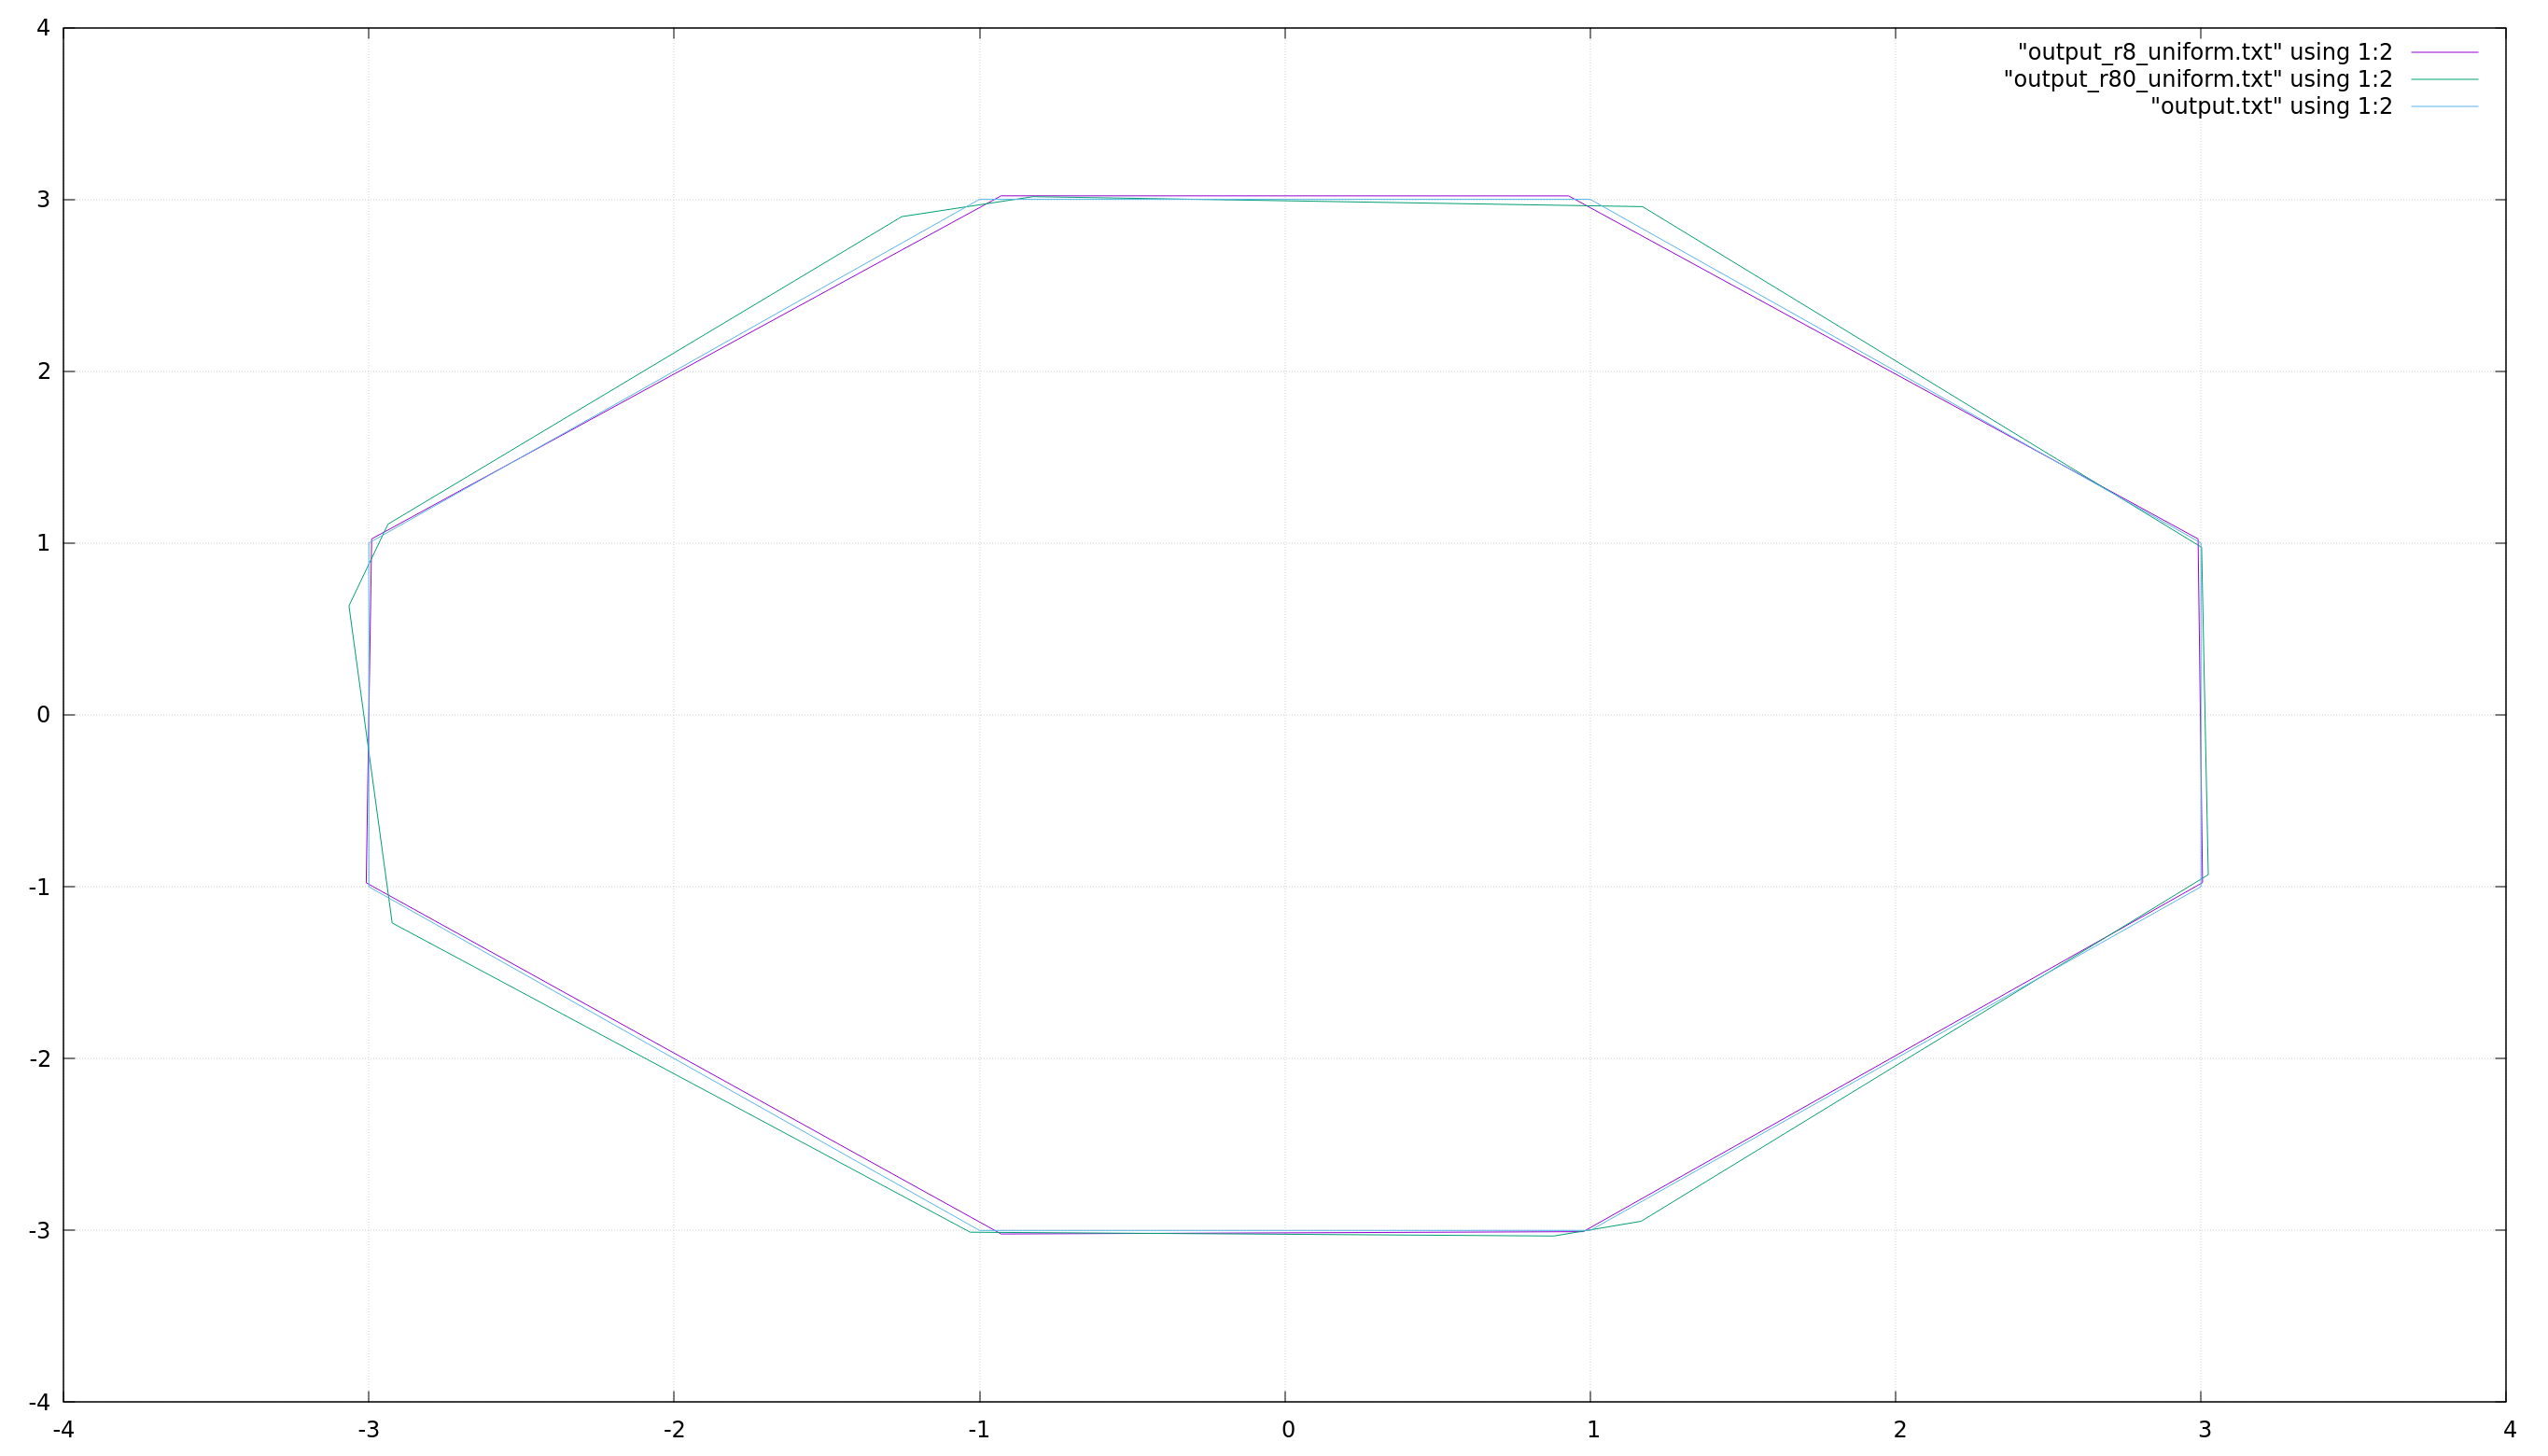
\includegraphics[width=0.8\linewidth]{output_uniform_compare.png}
    \caption{Сравнение восстановленных методом "ближайших соседей"\ многоугольников с эталоном}
\end{figure}

Разница с эталоном для r8:

\[
\mathrm{MSE} = 0.00593976327080012
\]
\[
d_{\max} = 0.07730644761395526
\]

Разница с эталоном для r80:

\[
\mathrm{MSE} = 0.008201129670586112
\]
\[
d_{\max} = 0.12613946706363163
\]

Разница r8 и r80 (рост ошибок):

\[
\mathrm{MSE} = 0.000653811595547378
\]
\[
d_{\max} = 0.05133493482377407
\]

Для метода "ближайших соседей":

Разница с эталоном для r8:

\[
\mathrm{MSE} = 0.0022225458187906766
\]
\[
d_{\max} = 0.07368993797203806
\]

Разница с эталоном для r80:

\[
\mathrm{MSE} = 9.809287370118973
\]
\[
d_{\max} = 4.555332917009146
\]

Разница r8 и r80 (рост ошибок):

\[
\mathrm{MSE} = 9.85429007201206
\]
\[
d_{\max} = 4.618806375149211
\]

Заметим, что метод ближайших соседей может быть улучшен, особенно для симметричных фигур. Пусть функция $r(\alpha)$ является периодической и содержит выраженные экстремумы (максимумы и минимумы), которые естественным образом разбивают её на интервалы.

Разобьём область определения $\alpha \in [0, 2\pi]$ на зоны, границами которых служат ближайшие минимумы функции. В каждой такой зоне локализуются соответствующие максимумы.

Для симметричных фигур (например, восьмиугольника) число таких зон равно числу осей симметрии, то есть $8$, и функция $r(\alpha)$ представляется как набор локальных сегментов:

\[
r(\alpha) = \bigcup_{i=1}^{N} r_i(\alpha), \quad N = 8.
\]

Для каждой зоны применяется метод ближайших соседей, при котором число итераций сглаживания $k_i$ подбирается индивидуально:

\[
k_i = \arg\min_{k} E_i(k) \ge 5 \ \text{(нижний порог)}
\]

где $E_i(k)$ — ошибка совпадения максимумов в $i$-й зоне между зашумлённой и эталонной функцией.

Дополнительно вводится условие согласованности: если минимальная ошибка совпадения максимумов равна $e_{\min}$, то она распространяется на все зоны:

\[
e_i = e_{\min}, \quad \forall i \in \{1, \dots, N\}.
\]

Таким образом, итоговый критерий выбора оптимального числа итераций определяется как:

\[
K^{*} = \arg\min_{k_1, \dots, k_N} \sum_{i=1}^{N} E_i(k_i),
\quad \text{при условии} \quad e_i = e_{\min}.
\]

\begin{figure}[H]
    \centering
    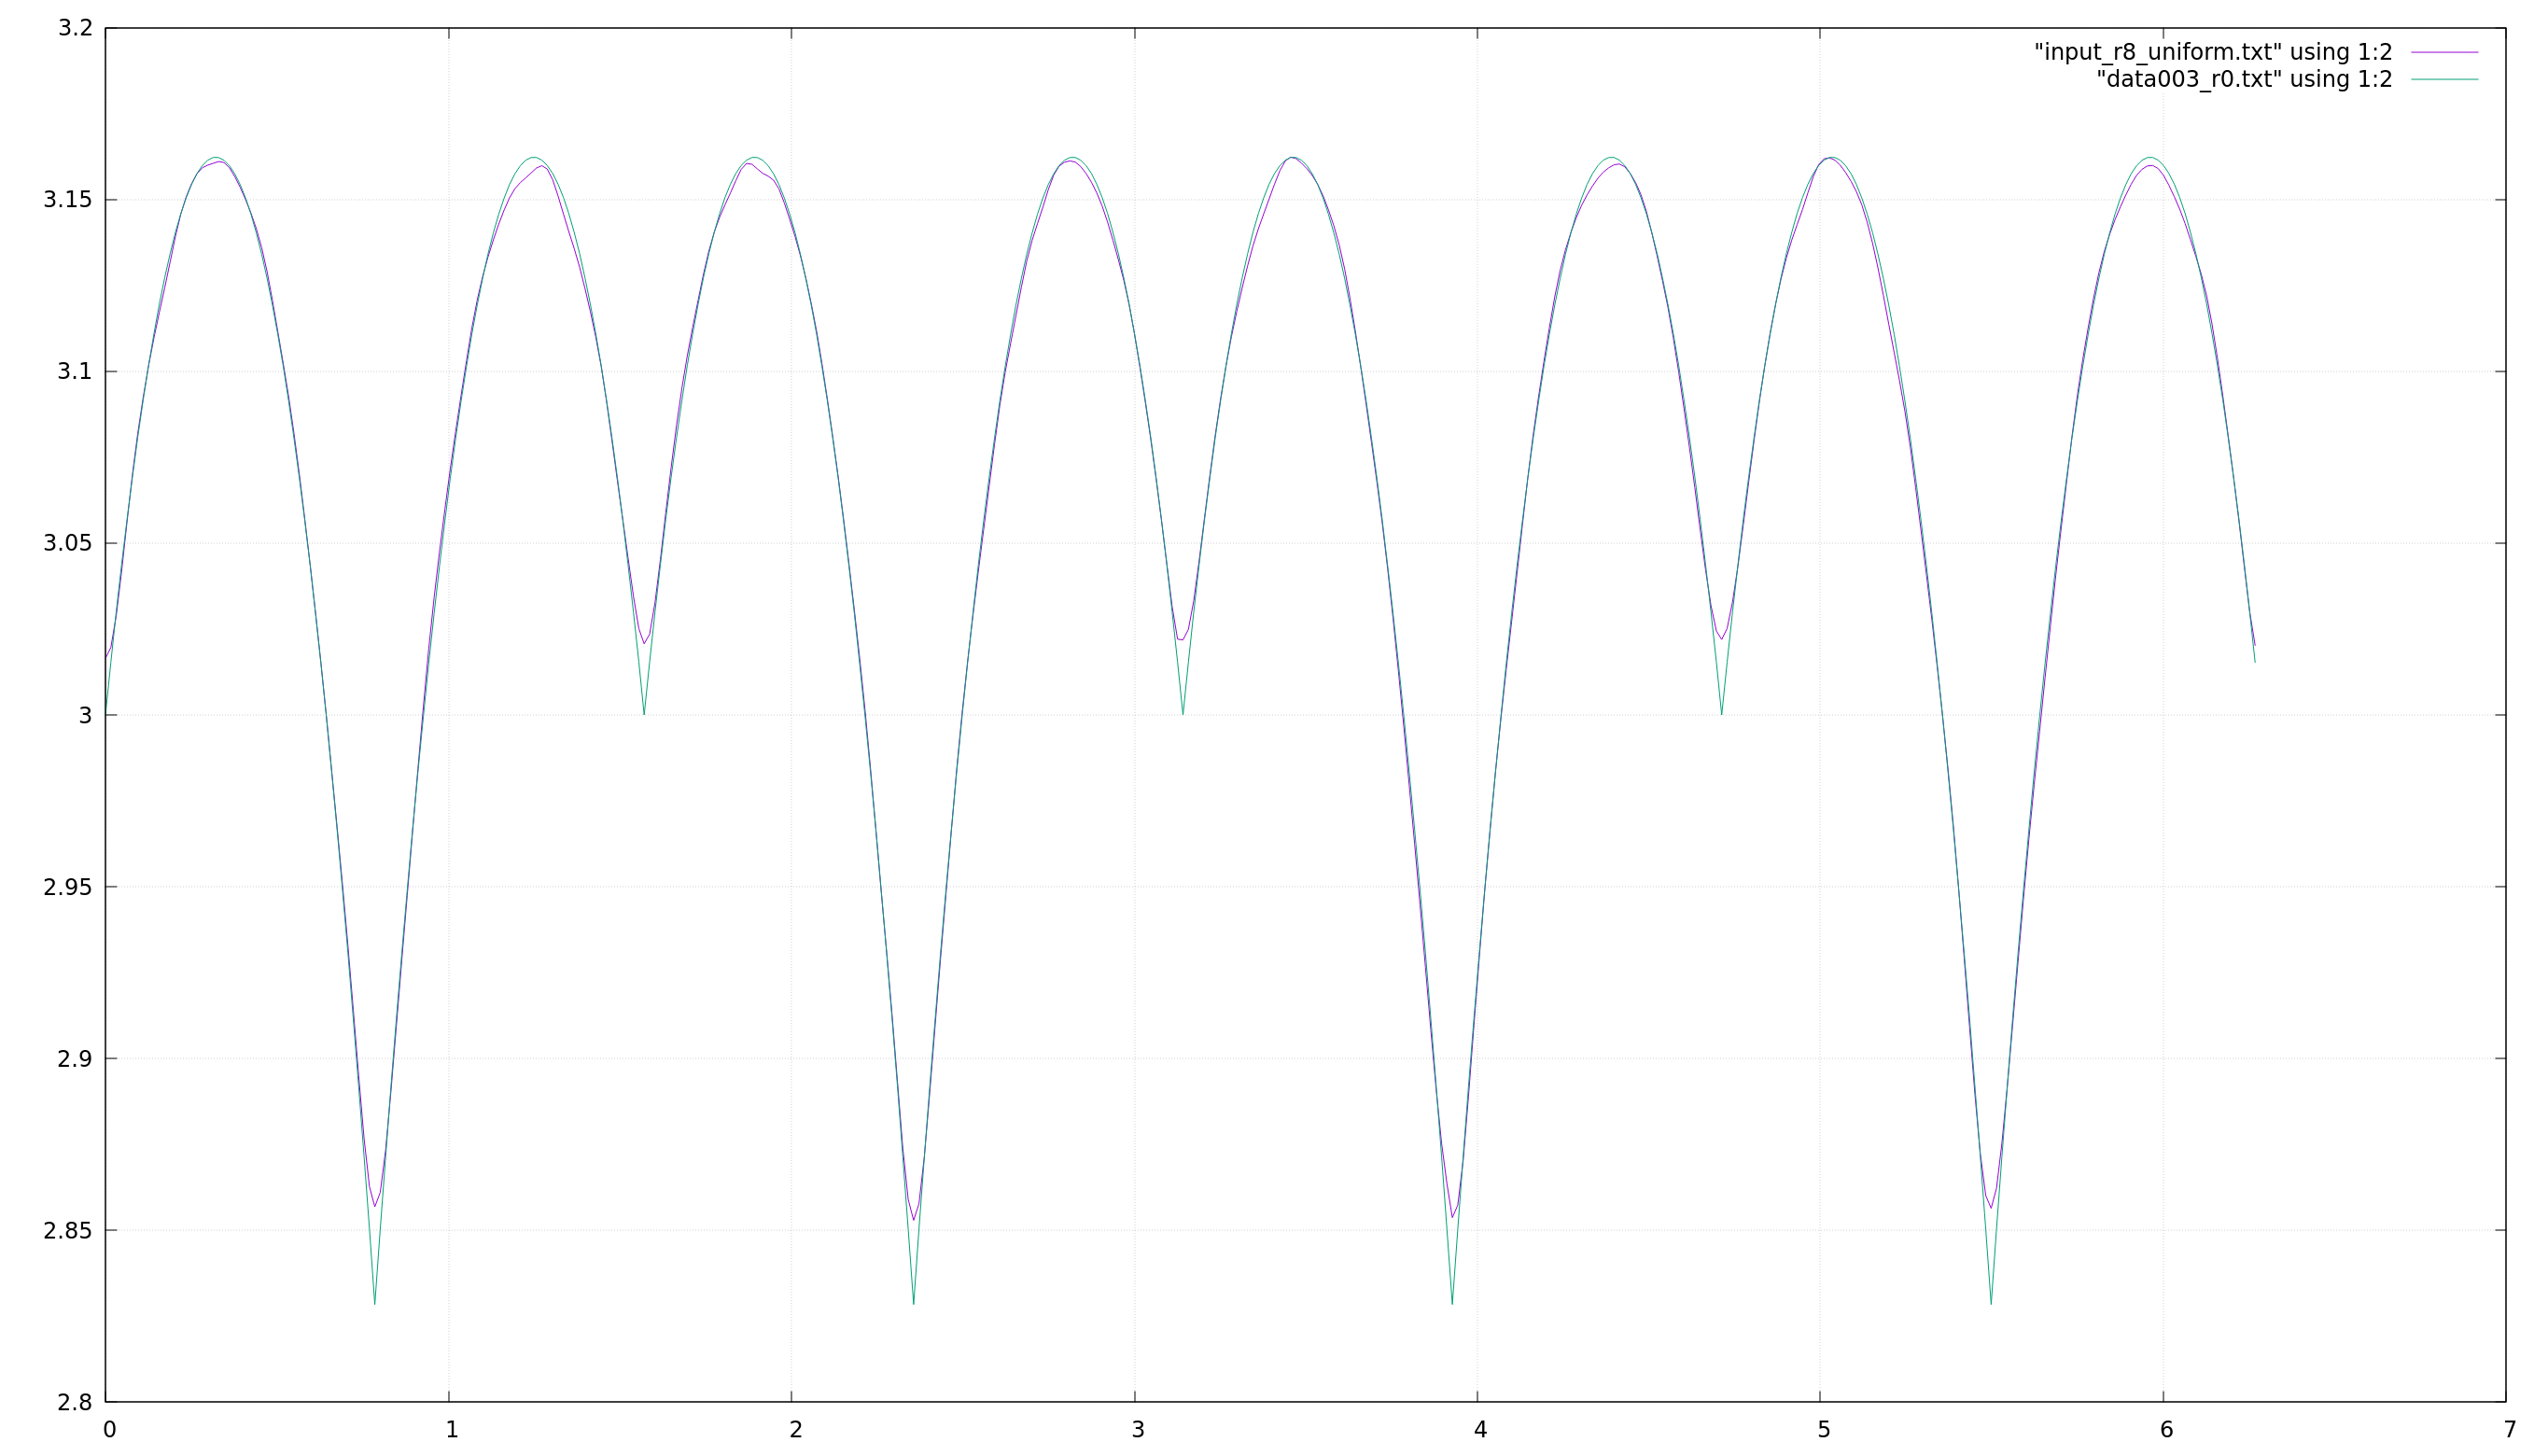
\includegraphics[width=0.8\linewidth]{input_r8_uniform_modified.png}
    \caption{Модифицированный метод "ближайших соседей"\ для r8 ($k_i = [5, 5, 5, 5, 7, 5, 5, 5],\ e_{min} \approx 0.001$)}
\end{figure}

\begin{figure}[H]
    \centering
    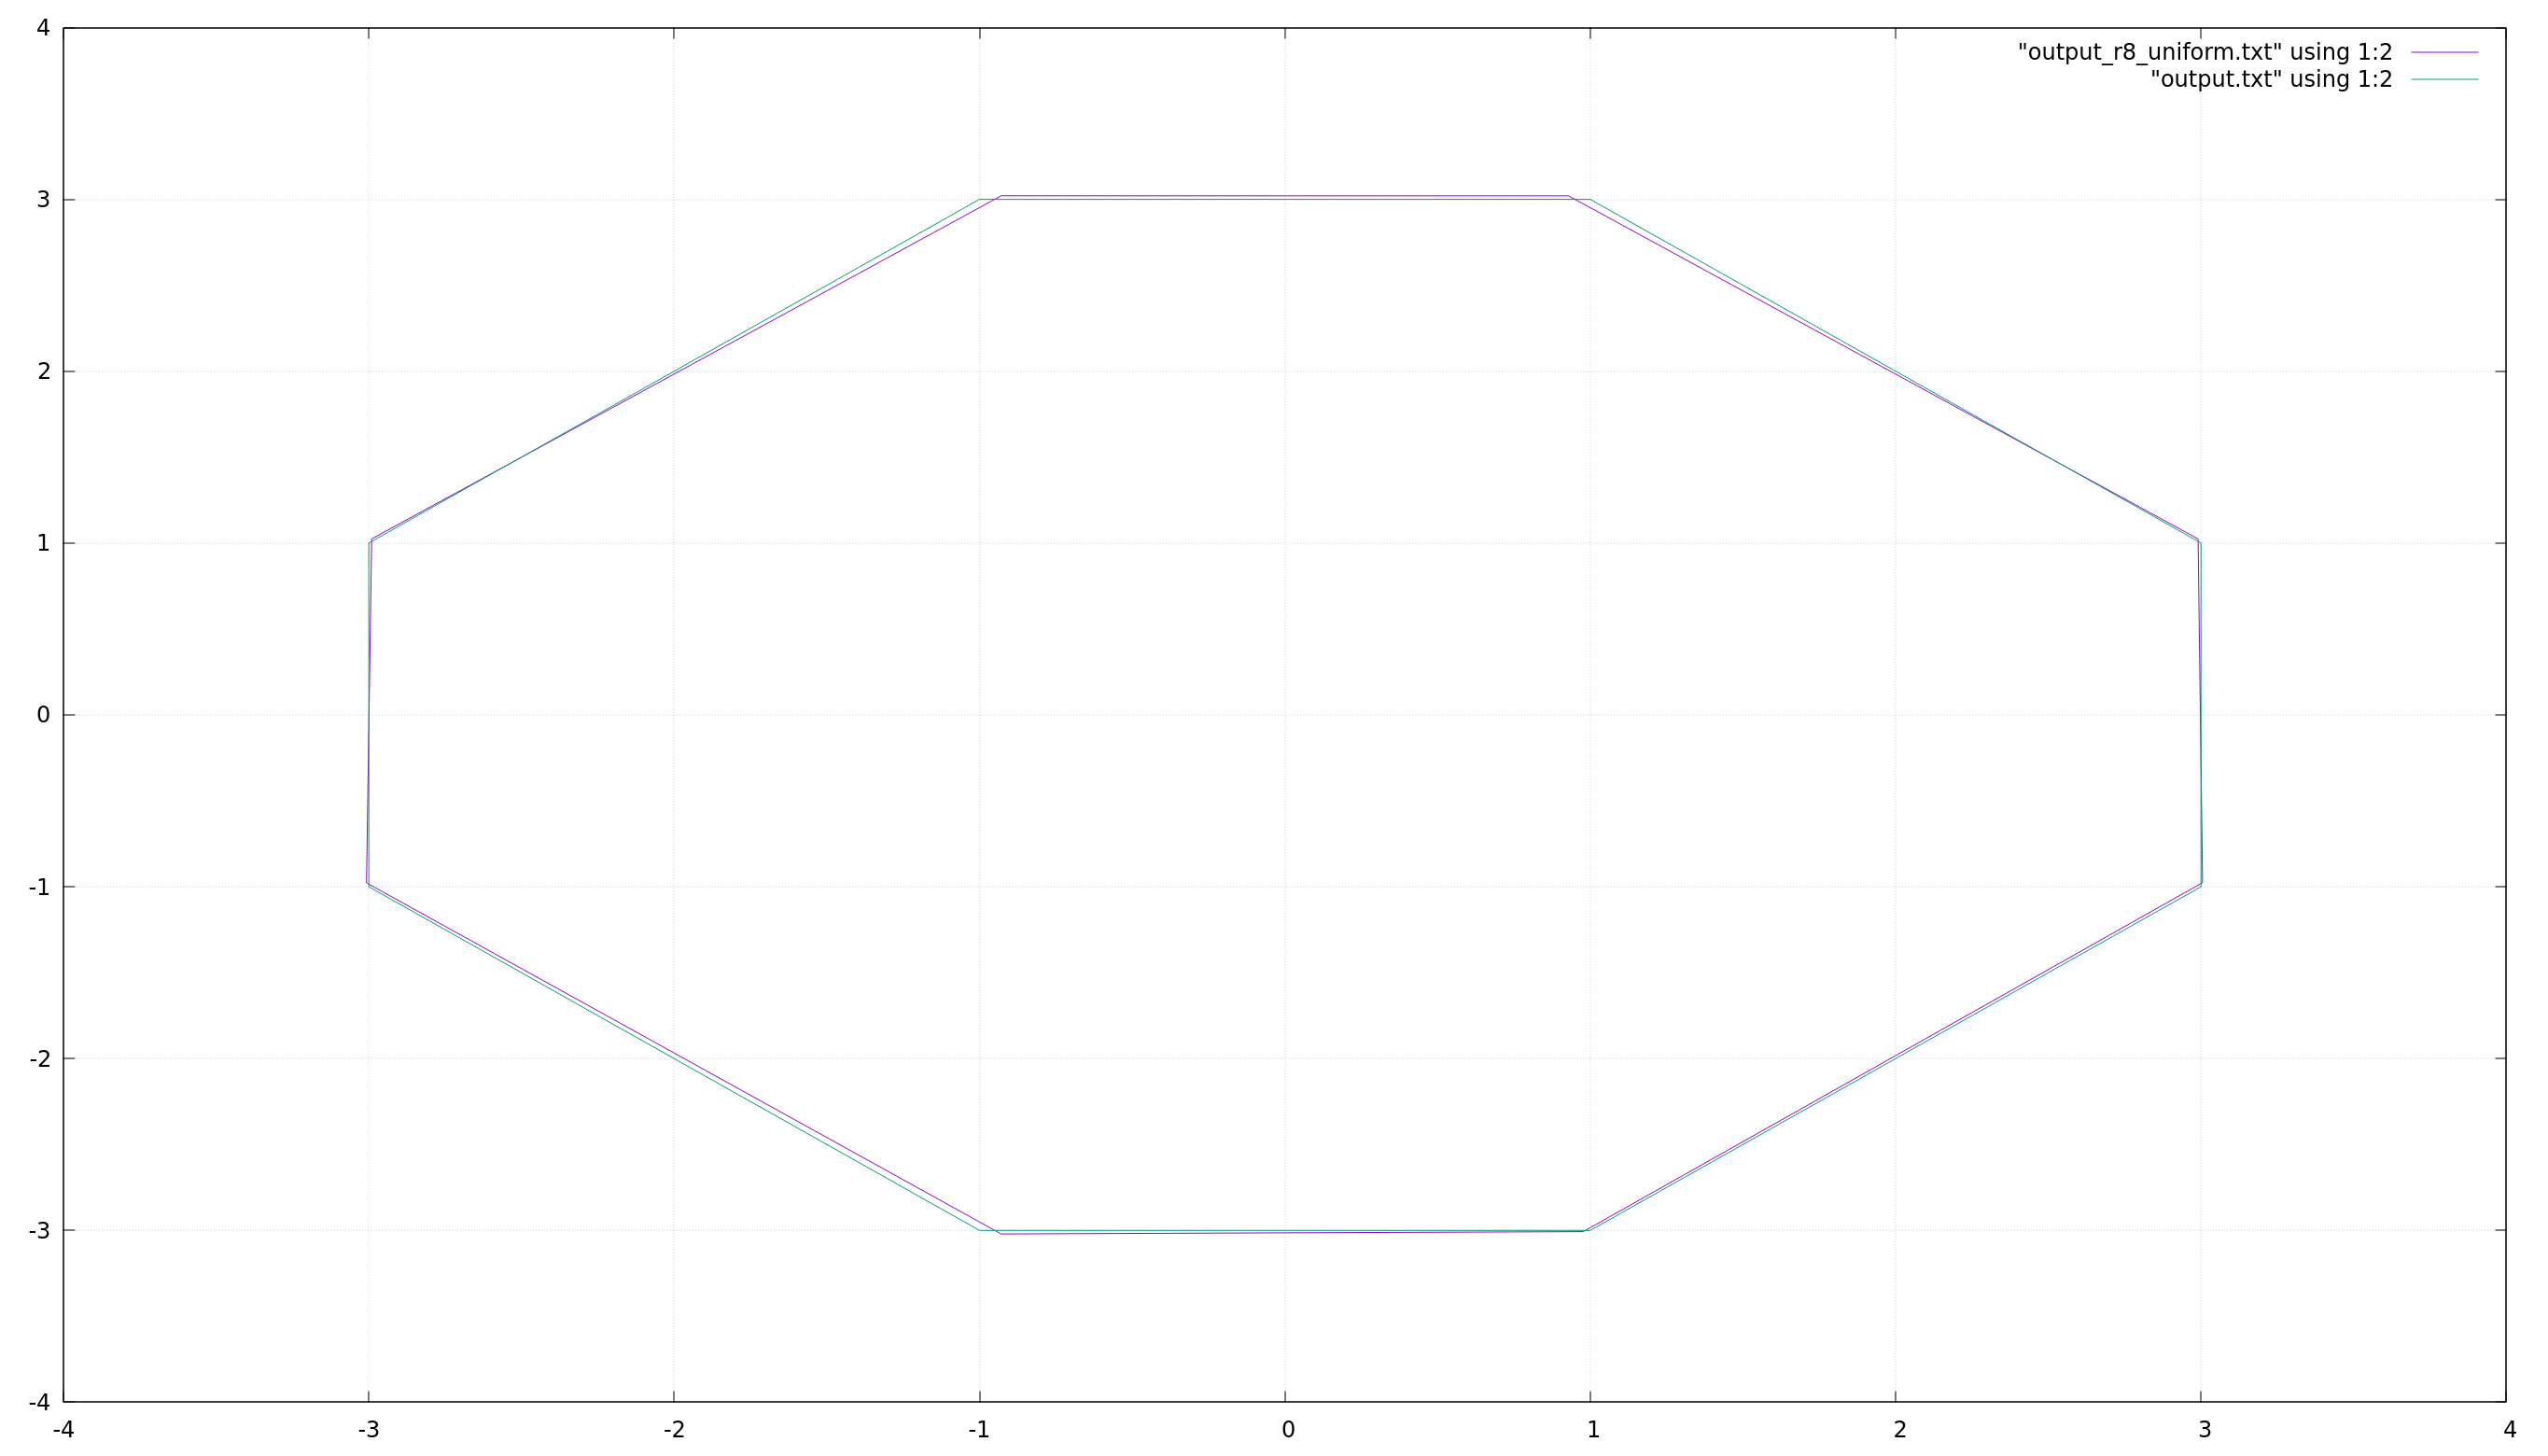
\includegraphics[width=0.8\linewidth]{output_uniform_modified.png}
    \caption{Сравнение с эталоном}
\end{figure}

Для модифицированного метода "ближайших соседей":

Разница с эталоном для r8:

\[
\mathrm{MSE} = 0.002222432354744529
\]
\[
d_{\max} = 0.07368993797203806
\]

Результаты тестирования в 3D ниже (визуализация --- $visualization.py$).

\begin{figure}[H]
    \centering
    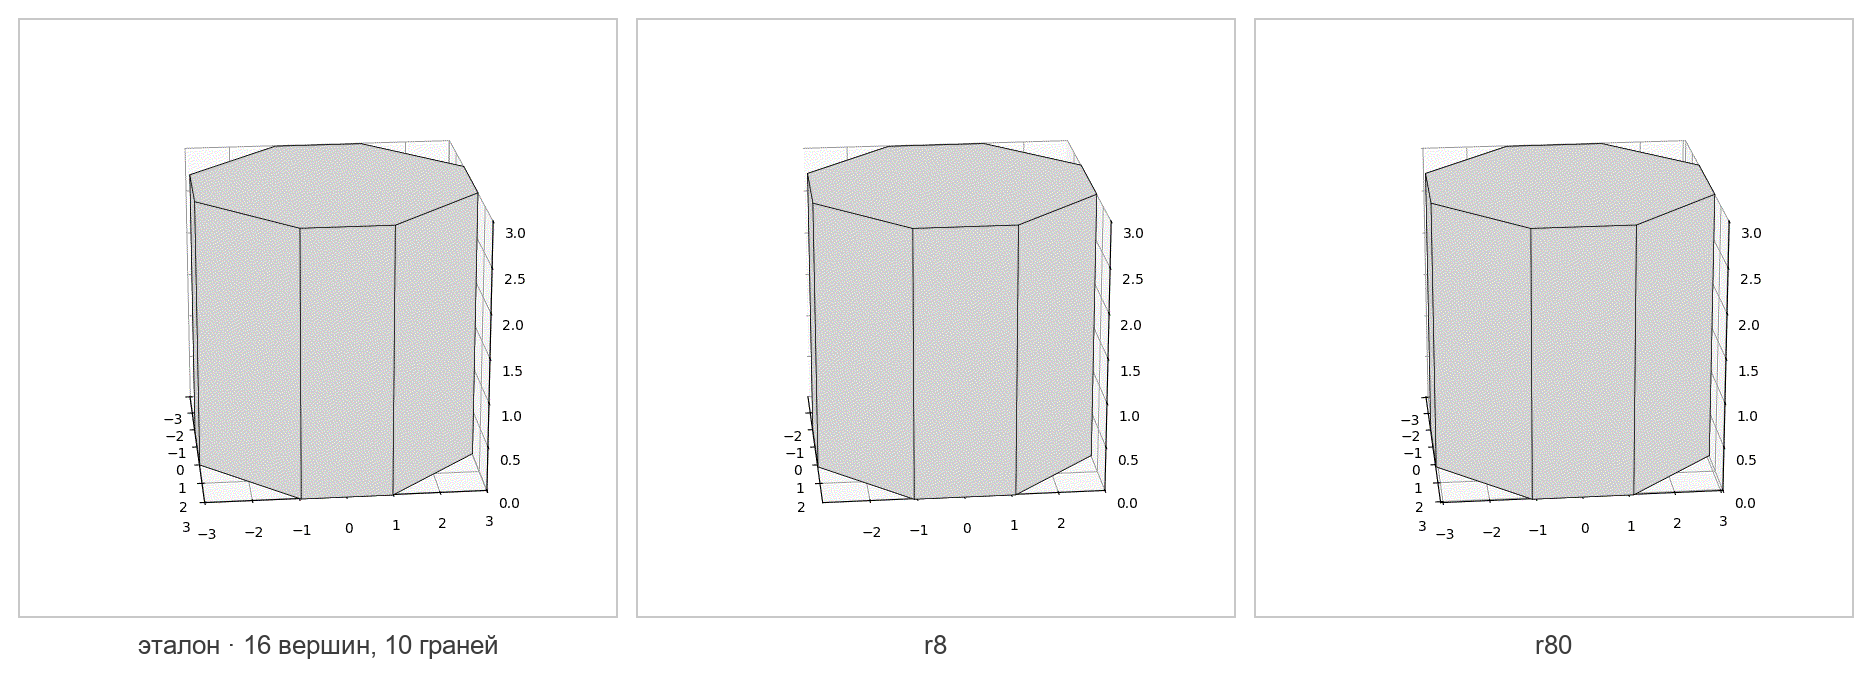
\includegraphics[width=0.95\linewidth]{fig3d_prism.png}
    \caption{Призма: эталон (16 вершин, 10 граней) и сглаженные r8- и r80-модели}
\end{figure}

Для каждой пары точек вычислялось евклидово расстояние:
\[
d_i =
\sqrt{
(x_i - \hat{x}_i)^2 +
(y_i - \hat{y}_i)^2 +
(z_i - \hat{z}_i)^2
},
\]
где:
\begin{itemize}
    \item $(x_i,y_i,z_i)$ — точка точной модели,
    \item $(\hat{x}_i,\hat{y}_i,\hat{z}_i)$ — восстановленная точка.
\end{itemize}
\[
\mathrm{RMSE} = \sqrt{\frac{1}{n}\sum_{i=1}^{n} \left[(x_i-\hat{x}_i)^2 + (y_i-\hat{y}_i)^2 + (z_i-\hat{z}_i)^2\right]}
\]

Разница с 3D-эталоном для r8:

\[
\mathrm{MSE} = 0.010425178540945794
\]
\[
\mathrm{RMSE} = 0.10210376359834046
\]
\[
d_{\max} = 0.10215679062837872
\]

Разница с 3D-эталоном для r80:

\[
\mathrm{MSE} = 0.01652071924772692
\]
\[
\mathrm{RMSE} = 0.12853295004677562
\]
\[
d_{\max} = 0.12996675489126402
\]

Разница r8 и r80 (рост ошибок в 3D):

\[
\mathrm{MSE} = 0.003355781266968158
\]
\[
\mathrm{RMSE} = 0.05792910552535882
\]
\[
d_{\max} = 0.05993940235644994
\]


\clearpage
\section{Трехмерные тела: генерация сечений, восстановление и подавление шума}

В разделе 5 трехмерный эксперимент был ограничен призмой: все слои имели одинаковый контур, поэтому форма сечения не менялась с высотой и проверялась только согласованность слоев по $z$. Ниже рассматриваются тела с переменным сечением --- правильные многогранники, у которых число вершин и форма контура зависят от высоты. Это показывает, что метод восстанавливает тело целиком, а не один контур, и позволяет сравнить методы подавления шума на разных типах сечений.

\subsection{Исходные тела}

Рассматриваются три правильных многогранника: октаэдр (6 вершин, 8 граней), икосаэдр (12 вершин, 20 граней) и додекаэдр (20 вершин, 12 граней), а также бриллиант --- тело с профилем огранки, у которого сечения меняются наиболее резко. Все тела выпуклые: для выпуклого тела опорная функция однозначно задает форму, а вершины сечения --- это локальные максимумы $R(\alpha)$.

Вершины задаются стандартными координатами через золотое сечение $\varphi=(1+\sqrt{5})/2$:
\begin{align*}
\text{октаэдр: } & (\pm 1,0,0),\ (0,\pm 1,0),\ (0,0,\pm 1); \\
\text{икосаэдр: } & (0,\pm 1,\pm\varphi),\ (\pm 1,\pm\varphi,0),\ (\pm\varphi,0,\pm 1); \\
\text{додекаэдр: } & (\pm 1,\pm 1,\pm 1),\ (0,\pm 1/\varphi,\pm\varphi),\
(\pm 1/\varphi,\pm\varphi,0),\ (\pm\varphi,0,\pm 1/\varphi).
\end{align*}

Каждое тело нормируется по описанной сфере (радиус 1), равномерно масштабируется до высоты $H=3$ и сдвигается по $z$ в отрезок $[0,H]$. Тело ставится вершиной вверх. Поворот не меняет геометрию, но избавляет от вырожденных сечений: если сверху оказывается горизонтальное ребро, у полюсов сечение превращается в узкую полоску, соседние вершины сближаются по углу и перестают разрешаться дискретной сеткой. После такой ориентации минимальный угловой зазор между соседними вершинами сечения составляет $90^\circ$ у октаэдра, $2.3^\circ$ у икосаэдра, $6.9^\circ$ у додекаэдра и $36^\circ$ у бриллианта, то есть во всех случаях больше шага сетки $0.5^\circ$.

Четвертое тело --- бриллиант короной вверх. Он не является правильным многогранником, но повторяет профиль огранки: площадка (радиус 0.8, высота 3), корона, рундист (радиус 1.7, высоты 2.05 и 1.95), павильон и колет (радиус 0.1, высота 0). Огранка десятигранная: 40 вершин и 32 грани, все горизонтальные сечения --- десятиугольники. Тело интересно тем, что ширина сечения сначала растет, затем резко падает, а у колета сечение становится совсем маленьким --- там относительный вклад шума максимален.

\begin{table}[H]
\centering
\caption{Параметры исследуемых тел}
\label{tab:3dbodies}
\begin{tabular}{|l|c|c|c|}
\hline
Тело & Вершин & Граней & Вершин в сечении \\
\hline
Октаэдр & 6 & 8 & 4 \\
Икосаэдр & 12 & 20 & 5--10 \\
Додекаэдр & 20 & 12 & 3--6 \\
Бриллиант & 40 & 32 & 10 \\
\hline
\end{tabular}
\end{table}

\subsection{Генерация горизонтальных точечных сечений}

Слои задаются с шагом $\Delta z = 0.05$:
\[
z_k=\left(k+\tfrac12\right)\Delta z,\qquad k=0,\dots,59,
\]
то есть 60 сечений; полушаг сдвига гарантирует, что плоскость не проходит через вершину тела и сечение не вырождается в точку или ребро.

Для каждого слоя строится сечение тела плоскостью $z=z_k$, его вершины обозначим $P_j^{(k)}=(x_j^{(k)},y_j^{(k)})$. Направления наблюдения задаются дискретно:
\[
\alpha_i=i h,\qquad h=\frac{2\pi}{n},\qquad n=720,
\]
то есть с шагом $h=0.5^\circ$. Шаг выбран минимальным из практически приемлемых: он в 4.6 раза меньше наименьшего углового зазора между вершинами сечения ($2.3^\circ$ у икосаэдра), поэтому все вершины разрешаются, а объем данных остается компактным.

Для каждого направления вычисляется опорная функция сечения:
\[
R(\alpha_i,z_k)=\max_j\left(x_j^{(k)}\cos\alpha_i+y_j^{(k)}\sin\alpha_i\right).
\]
Шум добавляется к каждому значению:
\[
\widetilde R(\alpha_i,z_k)=R(\alpha_i,z_k)+\varepsilon,\qquad
\varepsilon=r_v\xi,\qquad \xi\in[-1,1],
\]
с теми же амплитудами, что и в 2D: $r_v=0.008$ (r8) и $r_v=0.08$ (r80). Шум независим для каждой пары $(\alpha_i,z_k)$ и моделирует ошибки измерений, дискретизацию и неточности восстановления контуров.

В результате для каждого тела и каждого уровня шума формируется файл из $60\times720=43\,200$ строк вида
\[
(\alpha_i,\ \widetilde R(\alpha_i,z_k),\ z_k),
\]
который подается на вход программе $reconstruct3D\_layers.py$. Всего девять файлов: $data3D\_\{octa,\allowbreak icosa,\allowbreak dodeca\}\_\{r0,\allowbreak r8,\allowbreak r80\}.txt$. Генерация выполняется программой $generate3D\_bodies.py$.

\subsection{Восстановление эталонных тел}

Восстановление выполняется по слоям независимо: внутри слоя для каждой точки $i$ считаются разности
\[
d_1=r_i-r_{i-1},\qquad d_2=r_{i+1}-r_i,
\]
и точка считается вершиной, если $d_1\ge 0$ и $d_2<0$. Координаты вершины:
\[
x_i=r_i\cos\alpha_i,\qquad y_i=r_i\sin\alpha_i,
\]
а $z$ берется из слоя. Совокупность вершин всех слоев --- облако точек, по которому строится выпуклая оболочка; визуализация выполняется программой $visualize3D\_bodies.py$.

Программа $reconstruct3D\_layers.py$ повторяет логику $reconstruct.py$, но обрабатывает каждый слой отдельно: исходный $reconstruct.py$ рассчитан на один контур и при подаче многослойного файла замкнул бы массив через границу слоев. Критерий поиска вершин при этом не меняется.

На точных данных (r0) восстанавливается 240 точек для октаэдра, 430 для икосаэдра, 312 для додекаэдра и 600 для бриллианта. Сравнение с аналитическими сечениями дает $\mathrm{MSE}\le 9.4\cdot 10^{-7}$: эталон восстанавливается практически точно, остаточная погрешность --- только ошибка дискретизации по углу. Эталонные тела показаны на рисунке~\ref{fig:3dref}.

\begin{figure}[H]
\centering
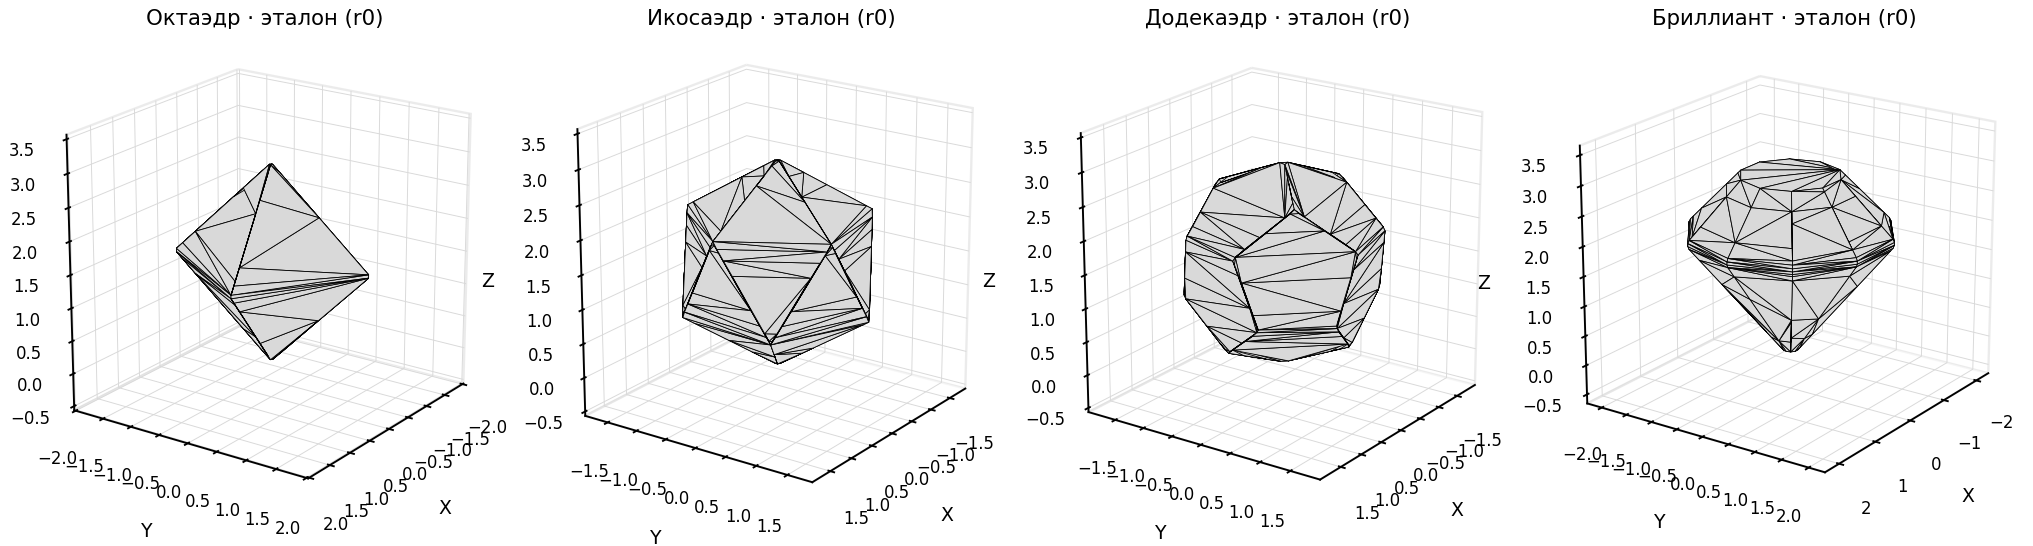
\includegraphics[width=0.95\linewidth]{fig3d_ref.png}
\caption{Эталонные тела, восстановленные по точным сечениям: октаэдр, икосаэдр, додекаэдр, бриллиант. Анимация вращения: body3D\_\{тело\}\_r0.gif}
\label{fig:3dref}
\end{figure}

\subsection{Восстановление зашумленных моделей}

Если подавление шума не выполнять, шумовые всплески сами становятся локальными максимумами. Число восстановленных точек вырастает с 240--600 до 12--14 тысяч: 12\,493 (октаэдр), 13\,204 (икосаэдр), 12\,235 (додекаэдр) и 13\,830 (бриллиант) при r8; 14\,374, 14\,388, 14\,382 и 14\,465 при r80. Оболочка покрывается тысячами мелких граней и «лохматится», а тело слегка увеличивается: шум дает смещения наружу, и максимум по слою выбирает самые выступающие точки. Ошибка при этом растет: MSE равен 0.00378 / 0.00140 / 0.00392 / 0.000293 для r8 и 0.01334 / 0.00912 / 0.01358 / 0.006382 для r80 (октаэдр / икосаэдр / додекаэдр / бриллиант). Зашумленные модели показаны на рисунке~\ref{fig:3dnoisy}.

\begin{figure}[H]
\centering
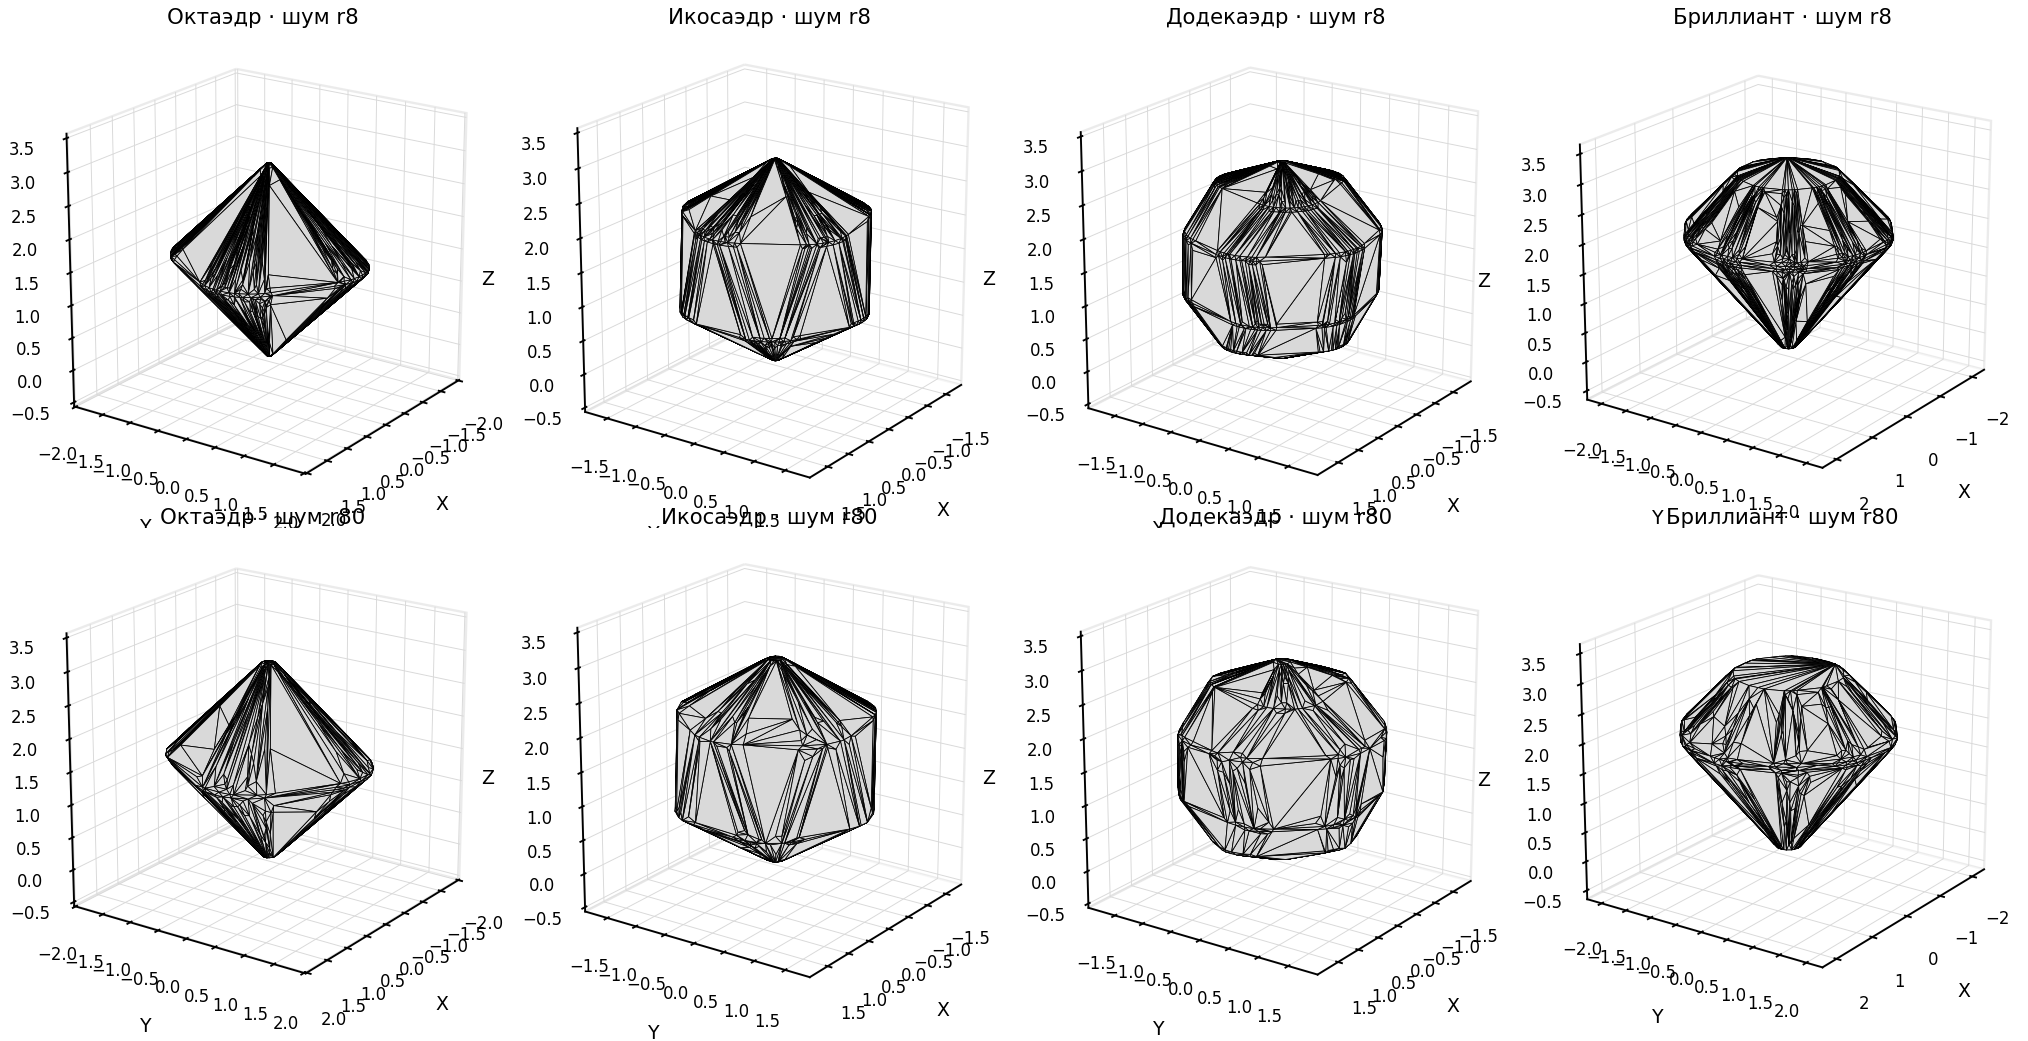
\includegraphics[width=0.9\linewidth]{fig3d_noisy.png}
\caption{Зашумленные модели: сверху r8, снизу r80. Анимация вращения: body3D\_\{тело\}\_r8.gif и body3D\_\{тело\}\_r80.gif}
\label{fig:3dnoisy}
\end{figure}

\subsection{Подавление шума по слоям}

Сглаживание применяется к каждому слою отдельно: функция $r(\alpha)$ определена в плоскости $z=z_k$, и смешивать значения разных высот нельзя.

\textbf{Ряд Фурье и МНК.} Для каждого слоя
\[
r(\alpha)\approx a_0+\sum_{m=1}^{M}\left(a_m\cos m\alpha+b_m\sin m\alpha\right),
\]
коэффициенты находятся из системы $Ac\approx r$ с матрицей
\[
A=\begin{bmatrix}
1 & \cos\alpha_1 & \sin\alpha_1 & \dots\\
1 & \cos\alpha_2 & \sin\alpha_2 & \dots\\
\vdots & \vdots & \vdots & \ddots
\end{bmatrix},
\qquad
c=\begin{bmatrix}a_0&a_1&b_1&\dots\end{bmatrix}^T,
\]
из условия $\|Ac-r\|^2\to\min$, то есть
\[
c=(A^TA)^{-1}A^Tr.
\]
Число гармоник принято $M=12$. Оно выбрано по максимальному числу вершин сечения: у икосаэдра сечение содержит до 10 вершин, а опорная функция многоугольника имеет изломы в направлениях нормалей к ребрам, поэтому ряд должен разрешать не только вершины, но и углы. Проверка при $M=8$ на тех же данных дала MSE в 2.4 раза хуже для икосаэдра (0.00180 против 0.00077 при r80) и почти не изменила результат для додекаэдра, где сечение содержит не более 6 вершин (0.00104 против 0.00099). В 2D при восьмивершинном сечении использовалось $M=8$ --- то же правило: число гармоник не меньше числа вершин.

\textbf{Метод «ближайших соседей».} Для каждого слоя
\[
\widetilde r(\alpha_i)=\frac{2r(\alpha_i)+r(\alpha_{i-1})+r(\alpha_{i+1})}{4},
\]
и это усреднение применяется $k$ раз. Как и в 2D, область разбивается на зоны между соседними минимумами, и для каждой зоны подбирается свое $k_i\in[5,30]$ по критерию совпадения максимумов с эталоном: $k_i=\arg\min_k E_i(k)$, нижний порог $k=5$. Подбор $k_i$ использует эталонную функцию, поэтому в этой постановке метод соседей настроен по эталону, тогда как МНК использует только число гармоник.

Результаты сглаживания показаны на рисунках~\ref{fig:3dfft} и~\ref{fig:3duni}.

\begin{figure}[H]
\centering
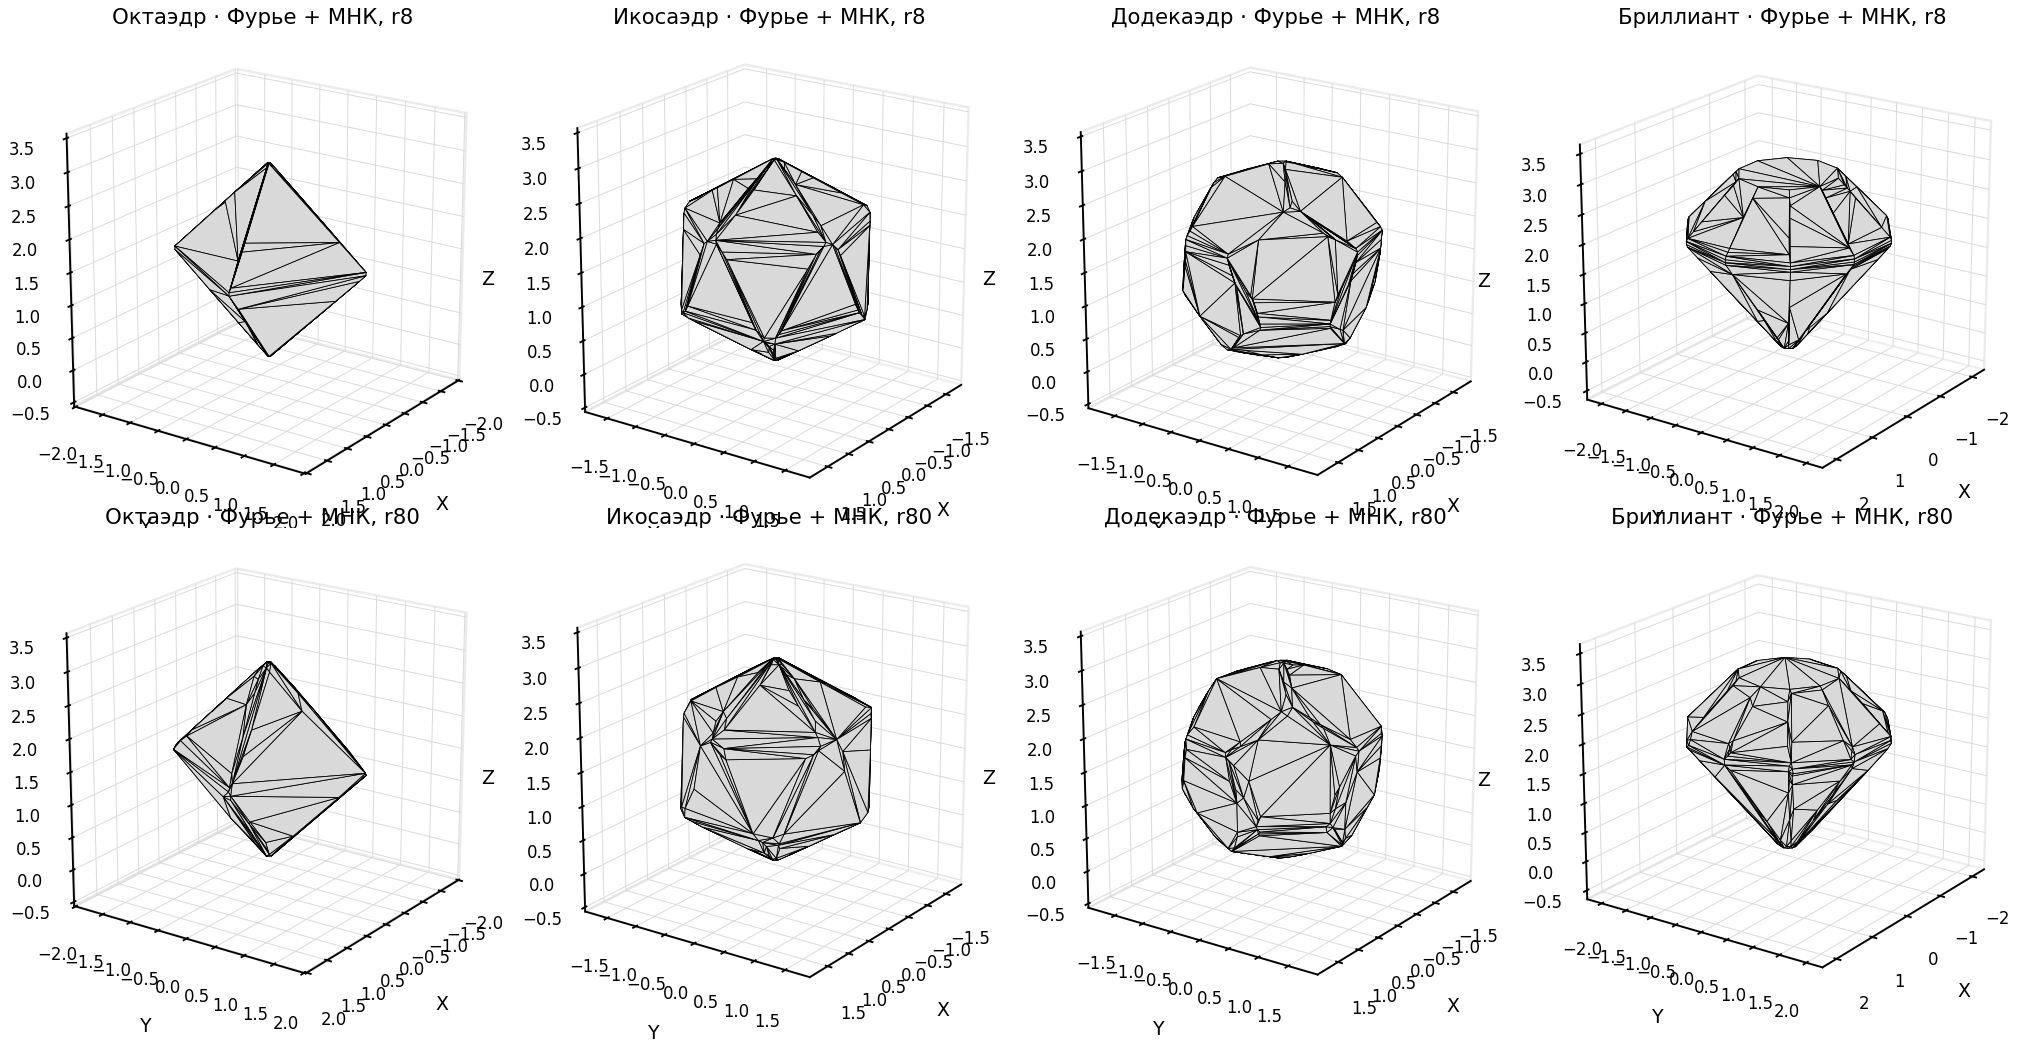
\includegraphics[width=0.9\linewidth]{fig3d_fft.png}
\caption{После подавления шума методом Фурье и МНК: сверху r8, снизу r80. Анимация: body3D\_\{тело\}\_fft\_r8.gif и body3D\_\{тело\}\_fft\_r80.gif}
\label{fig:3dfft}
\end{figure}

\begin{figure}[H]
\centering
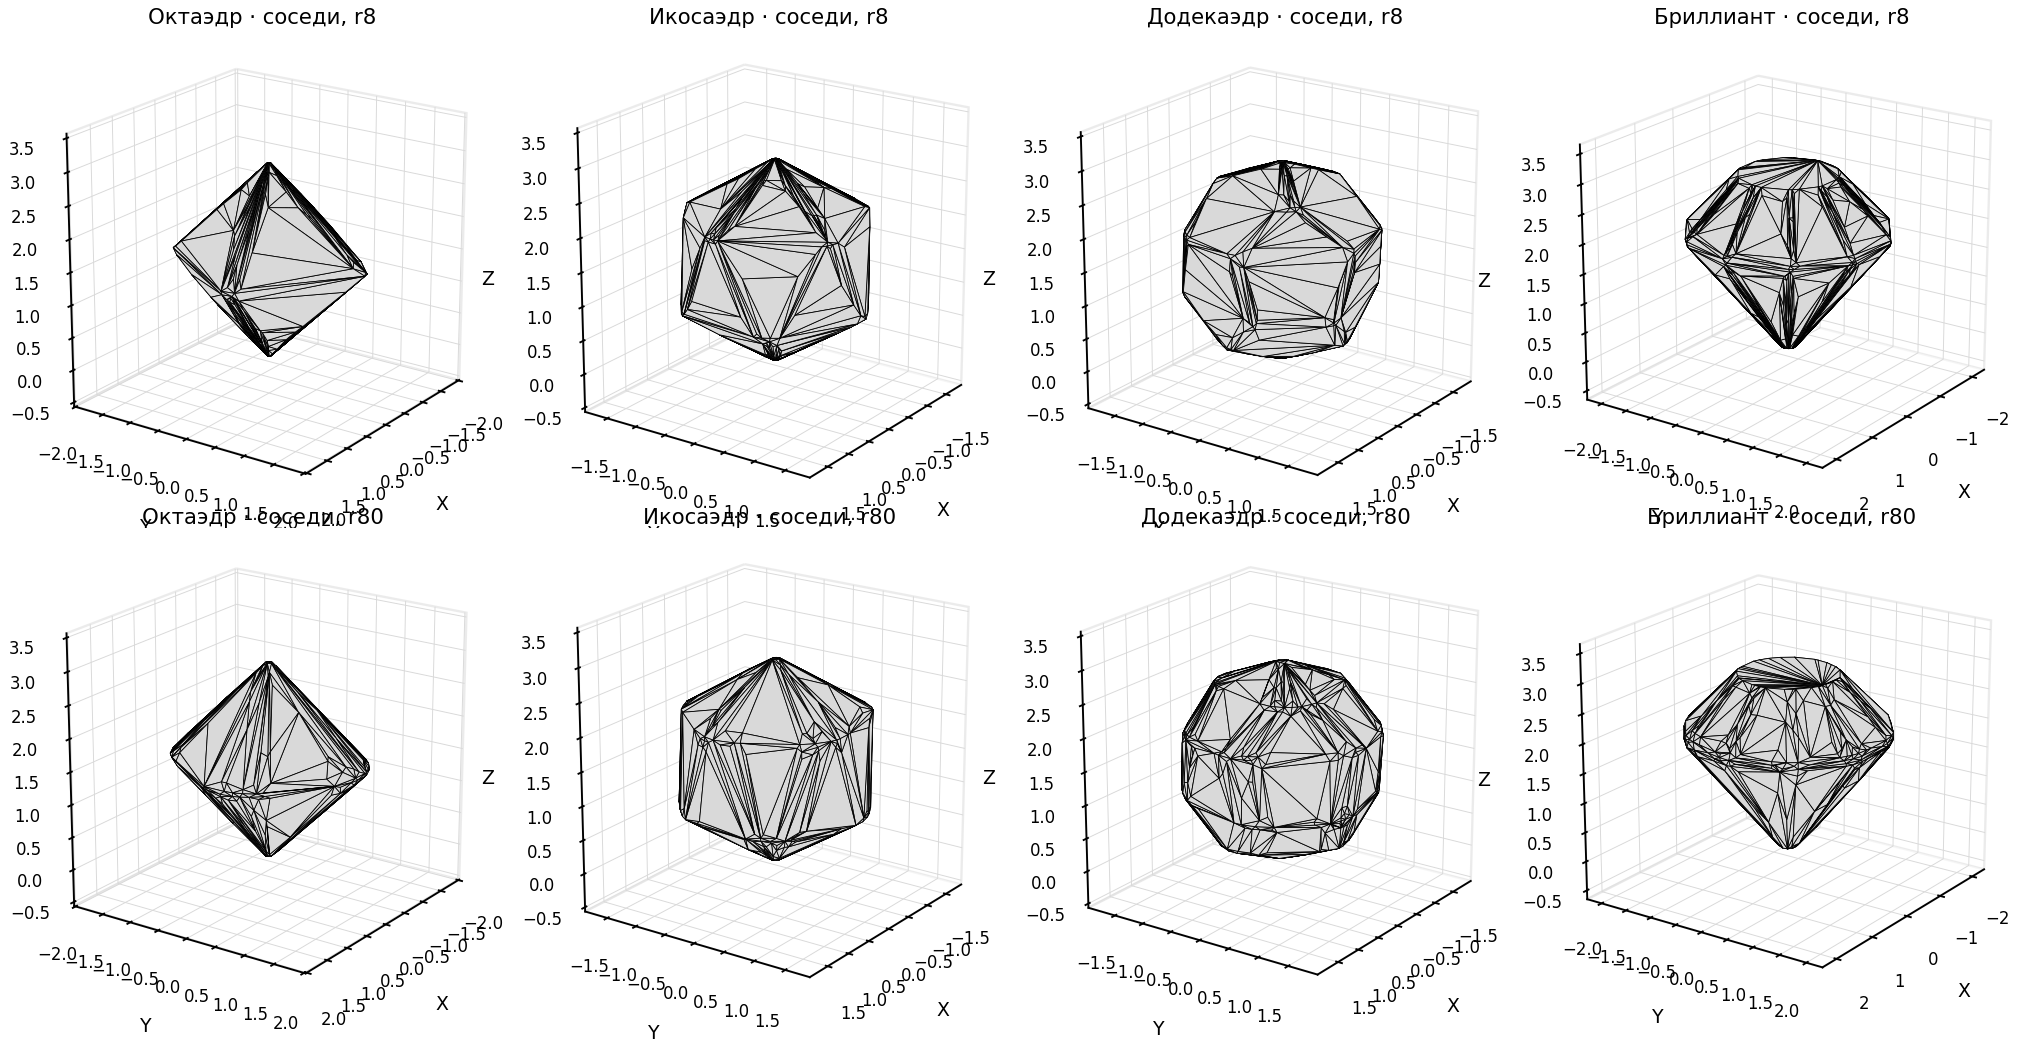
\includegraphics[width=0.9\linewidth]{fig3d_uni.png}
\caption{После подавления шума методом «ближайших соседей»: сверху r8, снизу r80. Анимация: body3D\_\{тело\}\_uni\_r8.gif и body3D\_\{тело\}\_uni\_r80.gif}
\label{fig:3duni}
\end{figure}

\subsection{Сравнение с эталоном}

Сравнение выполняется по опорной функции: для каждого слоя и каждого направления сетки считается отклонение
\[
\varepsilon(\alpha_i,z_k)=\widehat R(\alpha_i,z_k)-R(\alpha_i,z_k),
\]
\[
\mathrm{MSE}=\frac{1}{N}\sum\varepsilon^2,\qquad
\mathrm{RMSE}=\sqrt{\mathrm{MSE}},\qquad
d_{\max}=\max|\varepsilon|.
\]
Такой критерий не зависит от числа восстановленных вершин (после шума оно меняется) и напрямую измеряет отклонение формы. Результаты приведены в таблицах~\ref{tab:3dmse} и~\ref{tab:3ddmax}.

\begin{table}[H]
\centering
\caption{MSE относительно аналитического эталона}
\label{tab:3dmse}
\footnotesize
\begin{tabular}{|l|c|c|c|c|c|c|}
\hline
Тело & r8 & r80 & Фурье r8 & Фурье r80 & Соседи r8 & Соседи r80 \\
\hline
Октаэдр & 0.00378 & 0.01334 & 0.000014 & 0.000290 & 0.000563 & 0.00418 \\
Икосаэдр & 0.00140 & 0.00912 & 0.000205 & 0.000766 & 0.000271 & 0.00176 \\
Додекаэдр & 0.00392 & 0.01358 & 0.000380 & 0.000990 & 0.000568 & 0.00431 \\
Бриллиант & 0.000293 & 0.006382 & 0.000016 & 0.000149 & 0.000060 & 0.000508 \\
\hline
\end{tabular}
\end{table}

\begin{table}[H]
\centering
\caption{Максимальное отклонение $d_{\max}$}
\label{tab:3ddmax}
\footnotesize
\begin{tabular}{|l|c|c|c|c|c|c|}
\hline
Тело & r8 & r80 & Фурье r8 & Фурье r80 & Соседи r8 & Соседи r80 \\
\hline
Октаэдр & 0.223 & 0.288 & 0.013 & 0.095 & 0.115 & 0.238 \\
Икосаэдр & 0.135 & 0.203 & 0.105 & 0.165 & 0.089 & 0.154 \\
Додекаэдр & 0.252 & 0.313 & 0.061 & 0.194 & 0.146 & 0.265 \\
Бриллиант & 0.049 & 0.120 & 0.011 & 0.148 & 0.038 & 0.074 \\
\hline
\end{tabular}
\end{table}

Главный результат: МНК снижает MSE в 7--266 раз относительно зашумленной модели, метод «ближайших соседей» --- в 3--13 раз. При этом МНК возвращает и правильное число вершин: 247--600 точек против 240--600 у эталона, тогда как после соседей остается 871--3787 точек, то есть часть ложных максимумов сохраняется. По MSE МНК точнее соседей в 1.3--40 раз при обоих уровнях шума; при r80 разрыв составляет от 2.3 до 14 раз.

Максимальное отклонение ведет себя иначе. На икосаэдре при r8 метод соседей дает $d_{\max}=0.089$ против $0.105$ у МНК, хотя MSE у МНК в 1.3 раза ниже. Причина в том, что МНК сглаживает сильнее и «срезает» острые углы сечения, а $d_{\max}$ чувствителен к отдельным направлениям; по интегральной мере ошибки МНК точнее.

Отдельно отметим роль числа гармоник. При $M=8$, как в 2D, МНК работал хуже на десятиугольных сечениях икосаэдра: ряда не хватало, чтобы передать углы, и ошибка росла. Увеличение $M$ до 12 снимает это ограничение. Практическое правило: число гармоник должно быть не меньше максимального числа вершин сечения, а лучше --- с запасом, поскольку опорная функция многоугольника имеет изломы.

Итог раздела: на телах с переменным сечением оба метода восстанавливают форму, но МНК точнее по интегральной ошибке, устойчивее к росту шума и возвращает правильное число вершин; метод «ближайших соседей» проще, не требует выбора числа гармоник и в отдельных случаях дает меньшее максимальное отклонение, однако оставляет ложные вершины. Все анимации вращения для каждого тела и каждого варианта сохранены в каталоге out3D (файлы \textit{body3D\_\{тело\}\_\{вариант\}.gif}).

\subsection{Минимальный многогранник: автоматический режим}

По облаку точек можно строить не только выпуклую оболочку, но и минимальный многогранник --- модель с наименьшим числом граней, сохраняющую форму. В программе $visualization.py$ для этого предусмотрен автоматический режим: по оболочке выполняется квадратичная декцимация, доля оставшихся треугольников подбирается двоичным поиском так, чтобы площадь поверхности уменьшилась не более чем на $0.1\%$, а затем соседние треугольники с близкими нормалями (угол до $1^\circ$) сливаются в многоугольные грани. Число гармоник выбирается по источнику: 12 для демонстрационных тел и 32 для реальных моделей. Результат задается двумя числами --- числом вершин и числом граней.

Поясним термин. Декцимация (от латинского \textit{decimatio} --- «убавление на десятую часть»; в 3D-графике --- прореживание) это упрощение сетки: часть вершин и треугольников удаляется, а форма сохраняется. В русскоязычной литературе тот же прием чаще называют «упрощением сетки» или «понижением детализации». В квадратичной декцимации каждой вершине сопоставляется цена удаления --- сумма квадратов расстояний до плоскостей соседних граней; алгоритм последовательно стягивает ребро с наименьшей ценой и пересчитывает цену соседей, пока не останется заданное число треугольников. Поэтому «минимальный» многогранник --- это не произвольное огрубление, а наименее искажающее форму при заданном числе граней.

В приведенных ниже результатах после каждой декцимации оболочка перестраивается заново, и площадь для критерия $99.9\%$ считается уже по ней; это убирает уступы на плоских гранях (подробнее --- в разделе~8).

Автоматический режим применен ко всем 28 случаям: четырем телам и семи вариантам восстановления. Результаты приведены в таблице~\ref{tab:3dmin}, в ячейке указано число вершин и граней.

\begin{table}[H]
\centering
\caption{Минимальный многогранник: число вершин / граней (автоматический режим)}
\label{tab:3dmin}
\footnotesize
\begin{tabular}{|l|c|c|c|c|c|c|c|}
\hline
Тело & r0 & r8 & r80 & Фурье r8 & Фурье r80 & Соседи r8 & Соседи r80 \\
\hline
Октаэдр & 6/8 & 7/10 & 135/228 & 6/8 & 6/8 & 6/8 & 6/8 \\
Икосаэдр & 12/20 & 14/24 & 14/24 & 12/20 & 12/20 & 12/20 & 12/20 \\
Додекаэдр & 20/12 & 244/438 & 18/32 & 19/26 & 19/29 & 18/29 & 18/28 \\
Бриллиант & 17/25 & 258/417 & 228/370 & 14/24 & 13/22 & 14/22 & 14/23 \\
\hline
\end{tabular}
\end{table}

На эталонных данных режим точно восстанавливает октаэдр (6 вершин, 8 граней) и икосаэдр (12 вершин, 20 граней), причем после любого из двух методов сглаживания числа совпадают с исходными. Для додекаэдра эталон также восстанавливается точно (20 вершин, 12 граней), но после сглаживания получается 18--19 вершин и 26--29 граней: пятиугольные грани аппроксимируются несколькими почти компланарными треугольниками, и порог слияния $1^\circ$ их не объединяет. У бриллианта теряются мелкие элементы --- рундист и колет: их площадь мала, и критерий по площади их срезает (17 вершин и 25 граней вместо 40 и 32).

На зашумленных данных картина зависит и от уровня шума, и от размера исходных граней. У октаэдра грани крупные, поэтому при r8 шум не создает устойчивых фасетов и минимальный многогранник сводится к 7 вершинам и 10 граням. У додекаэдра грани мелкие, и уже при r8 сохраняются 244 вершины и 438 граней; при r80 у октаэдра --- 135 вершин и 228 граней. Отметим, что у додекаэдра при r80 число граней падает до 32: автоматический порог по площади выбирает более грубую модель ($2.8\%$ треугольников против $27\%$ при r8), то есть критерий по площади не монотонен по уровню шума.

\begin{figure}[H]
\centering
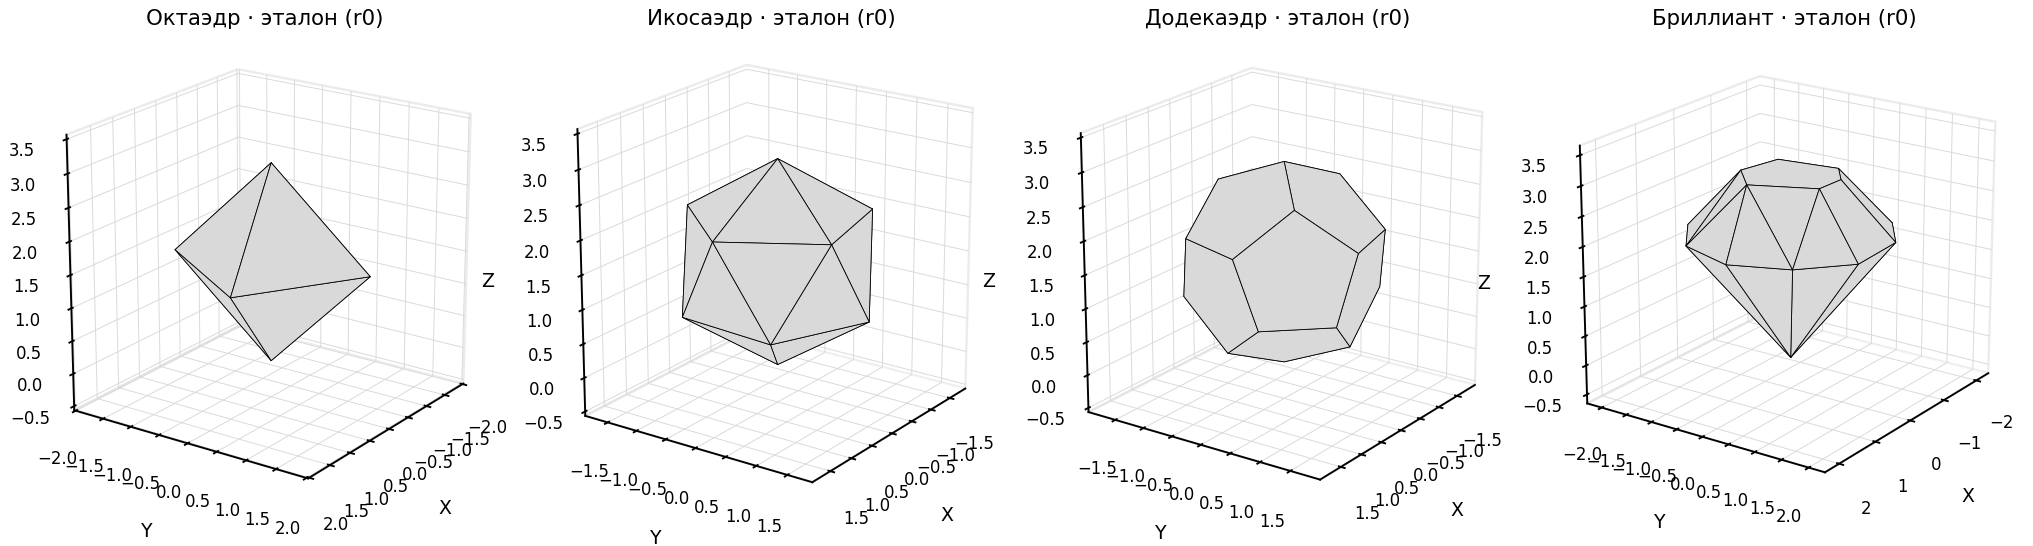
\includegraphics[width=0.95\linewidth]{fig3dmin_ref.png}
\caption{Минимальные многогранники по точным сечениям: октаэдр (6/8), икосаэдр (12/20), додекаэдр (20/12), бриллиант (17/25)}
\label{fig:3dminref}
\end{figure}

\begin{figure}[H]
\centering
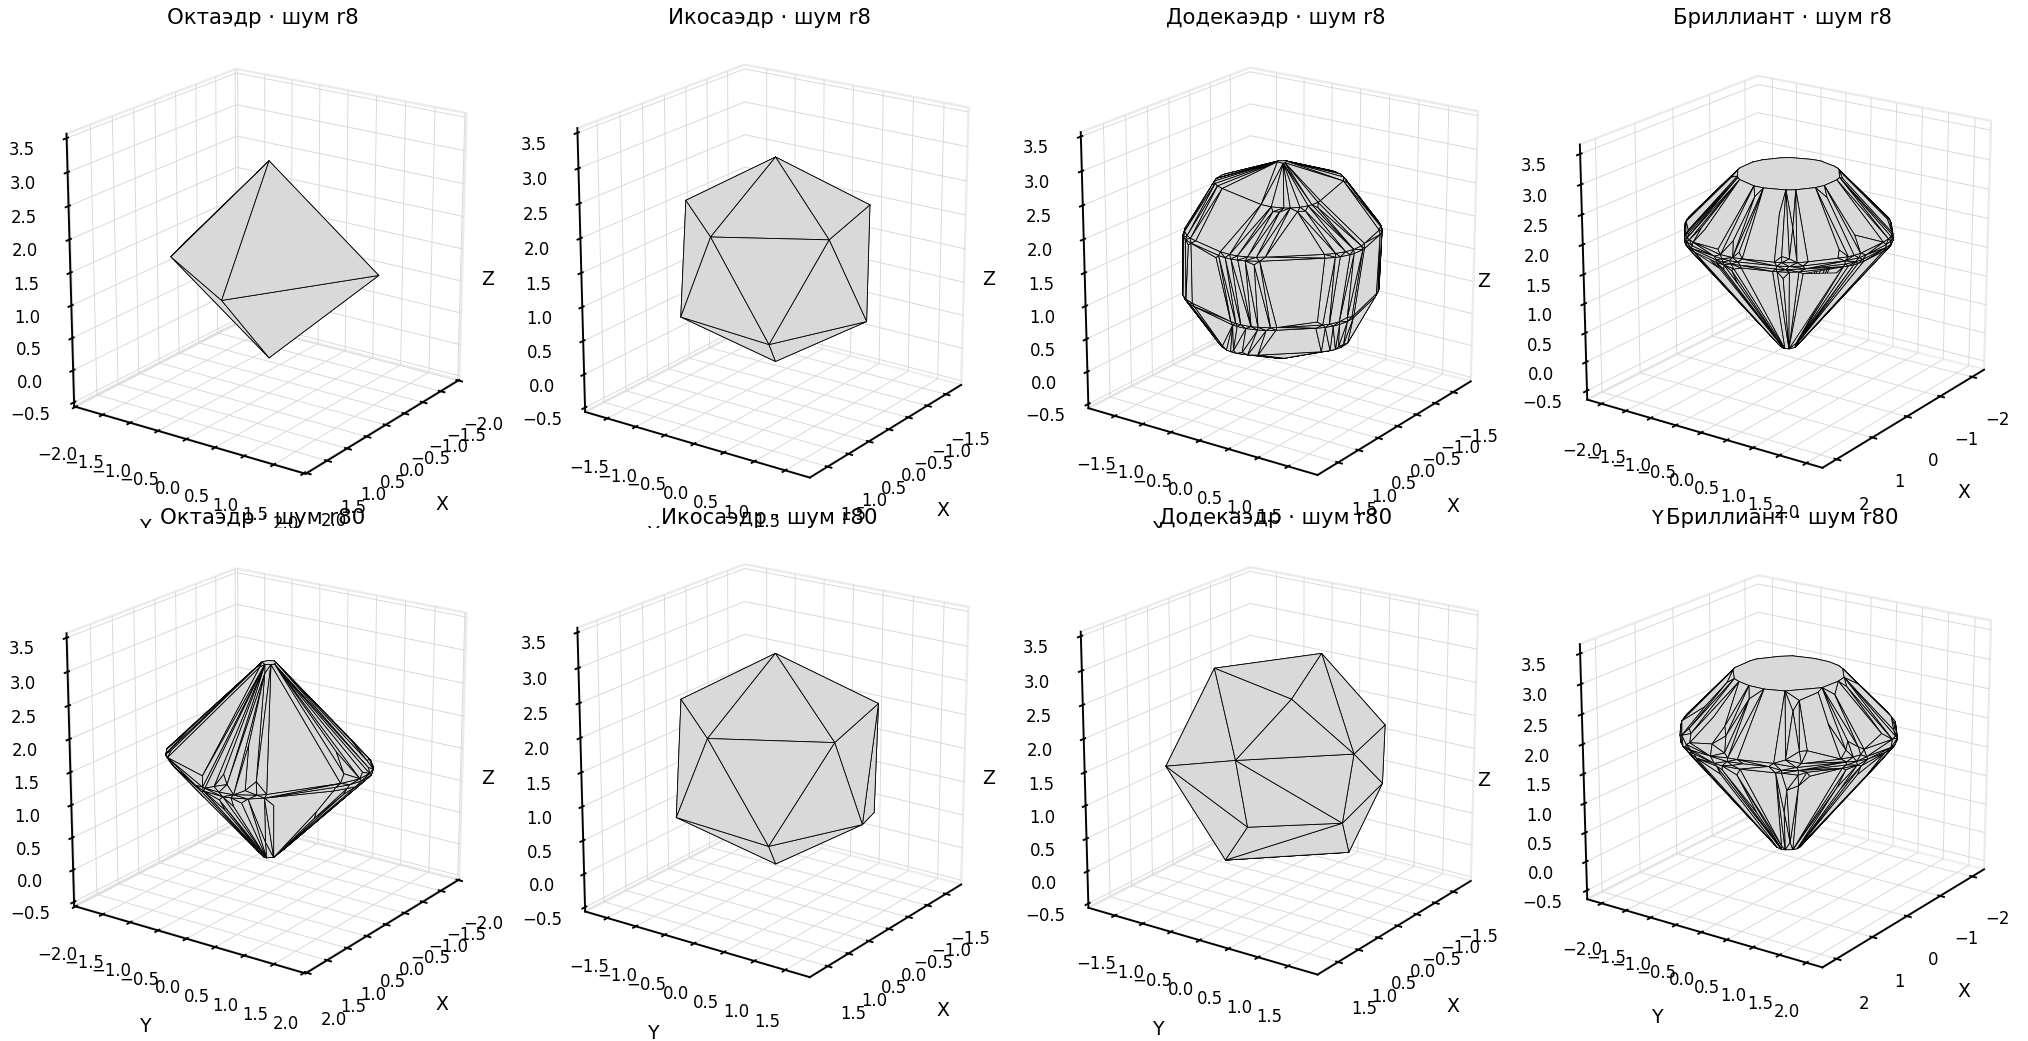
\includegraphics[width=0.9\linewidth]{fig3dmin_noisy.png}
\caption{Минимальные многогранники для зашумленных моделей: сверху r8, снизу r80}
\label{fig:3dminnoisy}
\end{figure}

\begin{figure}[H]
\centering
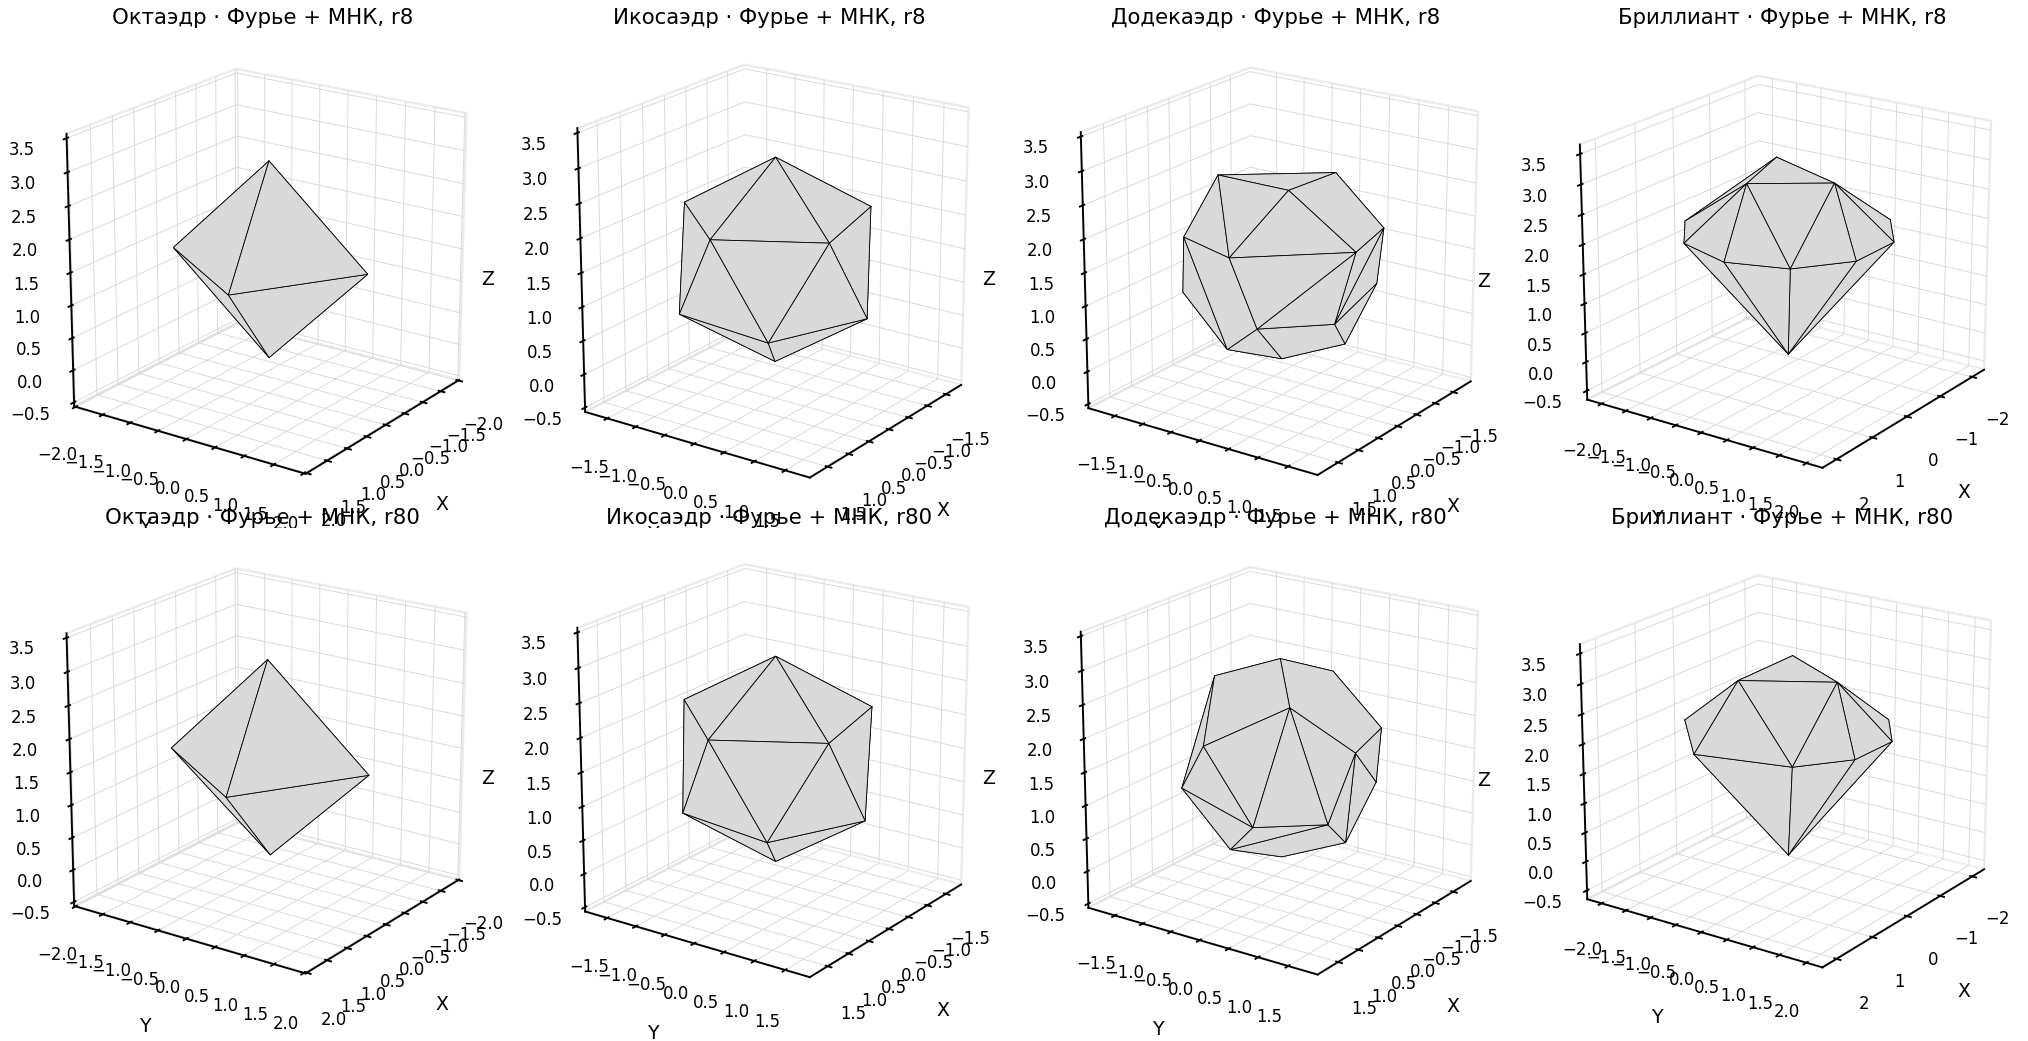
\includegraphics[width=0.9\linewidth]{fig3dmin_fft.png}
\caption{Минимальные многогранники после подавления шума методом Фурье и МНК: сверху r8, снизу r80}
\label{fig:3dminfft}
\end{figure}

\begin{figure}[H]
\centering
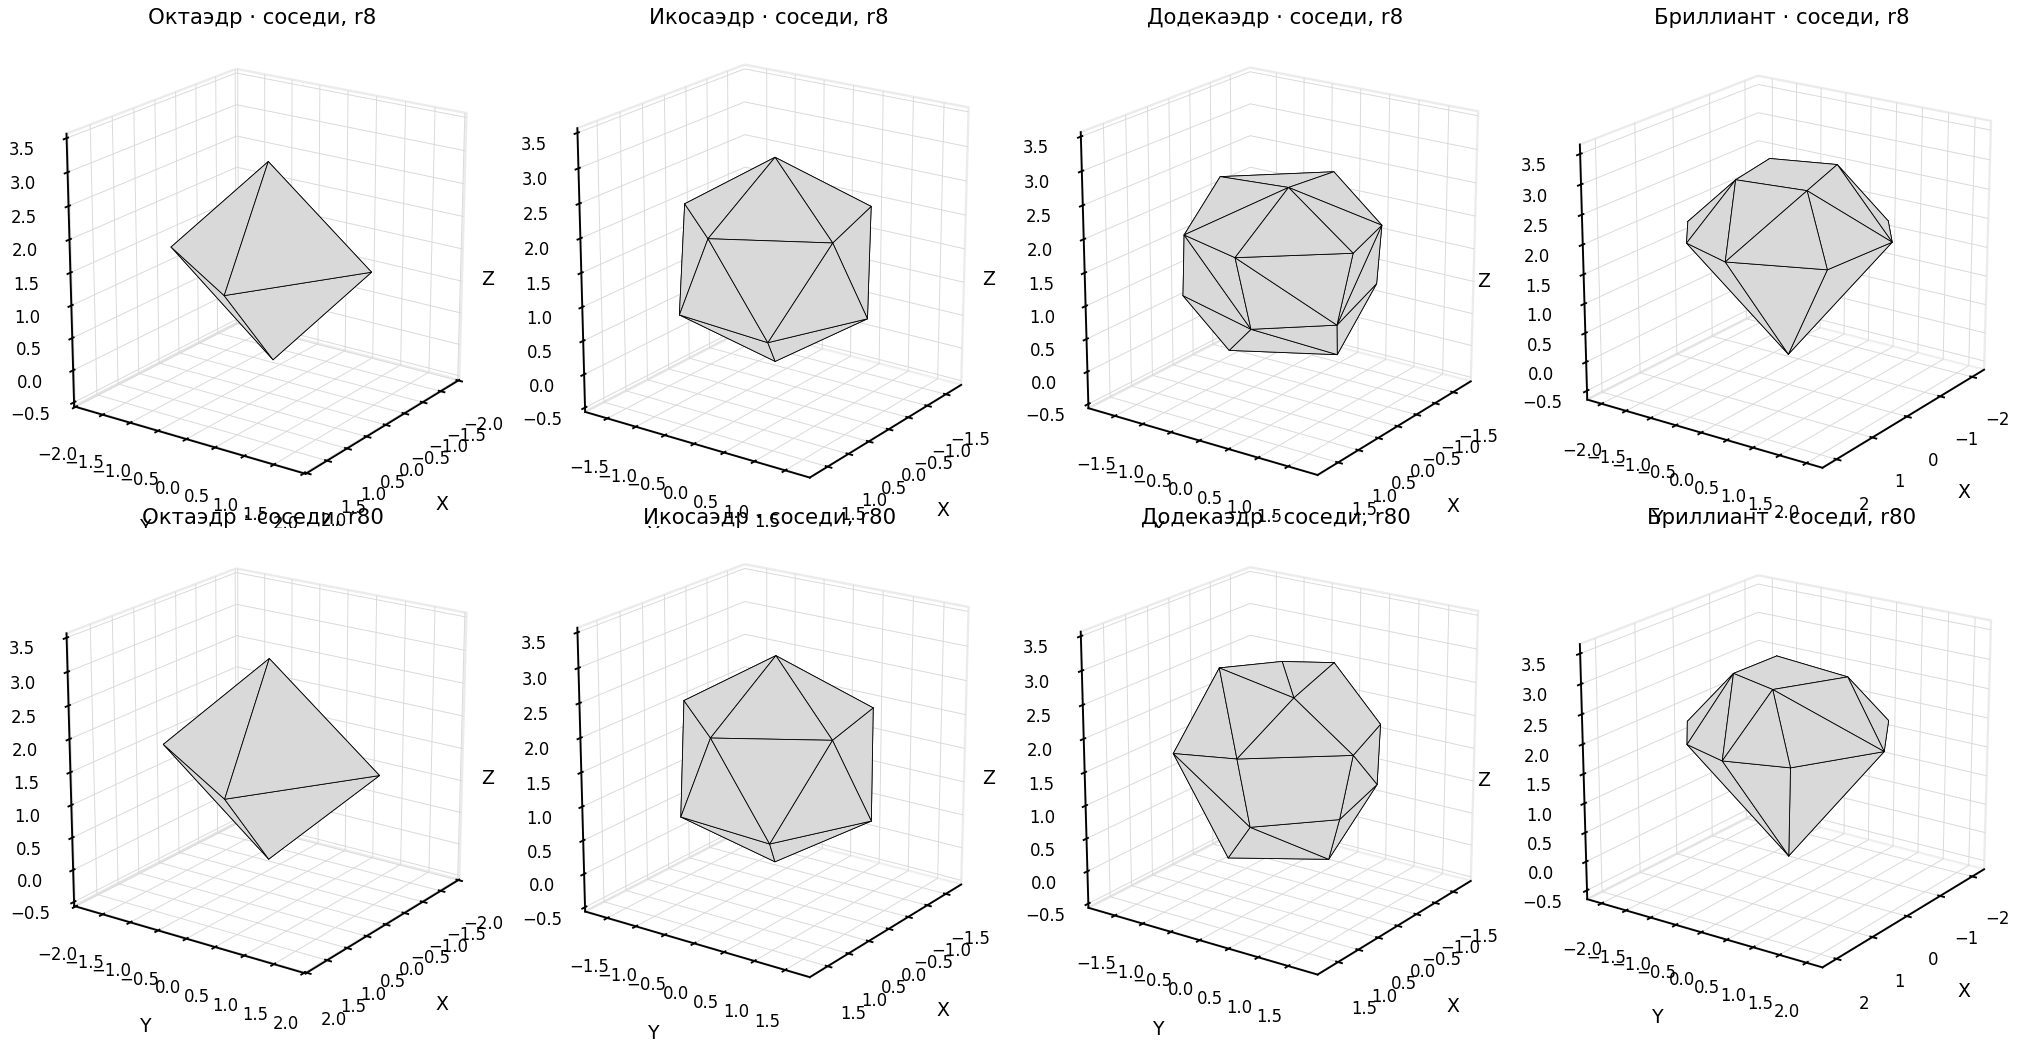
\includegraphics[width=0.9\linewidth]{fig3dmin_uni.png}
\caption{Минимальные многогранники после подавления шума методом «ближайших соседей»: сверху r8, снизу r80}
\label{fig:3dminuni}
\end{figure}

Вывод: автоматический режим дает компактное представление формы и точно восстанавливает тела с треугольными и четырехугольными гранями, но чувствителен к допуску по площади и порогу компланарности; для мелких и пятиугольных граней нужен меньший допуск. Анимации минимальных многогранников сохранены в каталоге out3D (файлы \textit{min3d\_\{тело\}\_\{вариант\}.gif}).

Все модели --- точные тела, оболочки и минимальные многогранники --- выгружены в формат OBJ в каталог $out3D/obj$: 60 файлов и манифест $manifest.csv$ с числом вершин и граней. OBJ открывается в Blender, MeshLab и большинстве 3D-редакторов; для просмотра без сторонних программ служит скрипт $view3D.py$, который строит модель в окне с вращением мышью.

\clearpage
\section{Реальные данные}

До сих пор все тела были синтетическими. Ниже тот же конвейер применяется к трем моделям, полученным сканером: $Reflect\_00001$, $Reflect\_10001$ и $Reflect\_20001$.

\subsection{Данные и подготовка}

Модели заданы выпуклыми многогранниками: 552, 436 и 490 вершин и 278, 220 и 247 граней соответственно. Габариты до нормировки: $6.4\times 6.4\times 4.0$, $4.5\times 8.3\times 2.5$ и $5.8\times 3.9\times 2.2$. Все вершины лежат на выпуклой оболочке, то есть тела выпуклые. В файлах площадка расположена внизу, а колет сверху, поэтому модели переворачиваются: корона оказывается наверху, высота нормируется к $H=3$, $z$ отсчитывается от нуля.

Сечения строятся так же: 60 слоев с шагом $0.05$ и 720 направлений с шагом $0.5^\circ$. Реальные сечения устроены сложнее синтетических: в них от 8 до 217 вершин (в среднем около 30), а минимальный угловой зазор между соседними вершинами достигает $0.02^\circ$ --- это микро-грани сканера, которые дискретная сетка не разрешает. Поэтому сечения считаются по ребрам сетки, а не по граням.

\subsection{Два режима восстановления}

Исходный прием --- считать вершины локальными максимумами $R(\alpha)$ --- опирается на то, что каждая вершина многоугольника является радиальным максимумом. Для правильных многогранников это так, для реальных огранок --- нет: у гладких овальных сечений радиальных максимумов всего 3--4 на слой. Проверка это подтверждает: на точных сечениях режим максимумов дает 1294 точки для первого образца (MSE $4.1\cdot10^{-5}$), но лишь 244 и 293 точки для второго и третьего, а ошибка возрастает до $0.12$ и $0.077$.

Поэтому для реальных данных используется обобщение: сечение восстанавливается как пересечение полуплоскостей
\[
\widehat K=\left\{x:\ x\cdot e(\alpha_i)\le R(\alpha_i)\ \ \forall i\right\},
\qquad e(\alpha)=(\cos\alpha,\ \sin\alpha)^T,
\]
то есть как тело, для которого измеренные значения $R(\alpha_i)$ являются опорными. На точных данных это обращение точное: MSE составляет $10^{-13}$, а максимальное отклонение --- $10^{-6}$.

\begin{table}[H]
\centering
\caption{Точные сечения: режим максимумов и обобщенное восстановление}
\label{tab:realmodes}
\footnotesize
\begin{tabular}{|l|c|c|c|}
\hline
Образец & Максимумы (точек / MSE) & Полуплоскости (точек / MSE) & min (вершин / граней) \\
\hline
1 ($Reflect\_00001$) & 1294 / $4.1\cdot10^{-5}$ & 43\,200 / $4.8\cdot10^{-14}$ & 95 / 147 \\
2 ($Reflect\_10001$) & 244 / $0.1197$ & 41\,883 / $2.3\cdot10^{-13}$ & 95 / 149 \\
3 ($Reflect\_20001$) & 293 / $0.0774$ & 42\,854 / $2.0\cdot10^{-13}$ & 101 / 151 \\
\hline
\end{tabular}
\end{table}

Обобщенное восстановление требует 720 точек на слой, поэтому минимальный многогранник получается крупнее, чем у синтетических тел: 95--101 вершина и 147--151 грань против 436--552 вершин и 220--278 граней исходной модели. Исходные модели и восстановленные по точным сечениям тела показаны на рисунках~\ref{fig:realtrue} и~\ref{fig:realr0}.

Автоматический режим (раздел 6.7) применен ко всем вариантам реальных данных: на рисунках этого раздела показаны именно минимальные многогранники, а не триангулированные оболочки. Для точных сечений они содержат 95--101 вершину и 147--151 грань; после сглаживания --- от 392 до 584 вершин и от 584 до 676 граней, потому что критерий по площади сохраняет мелкие грани сглаженной оболочки.

\begin{figure}[H]
\centering
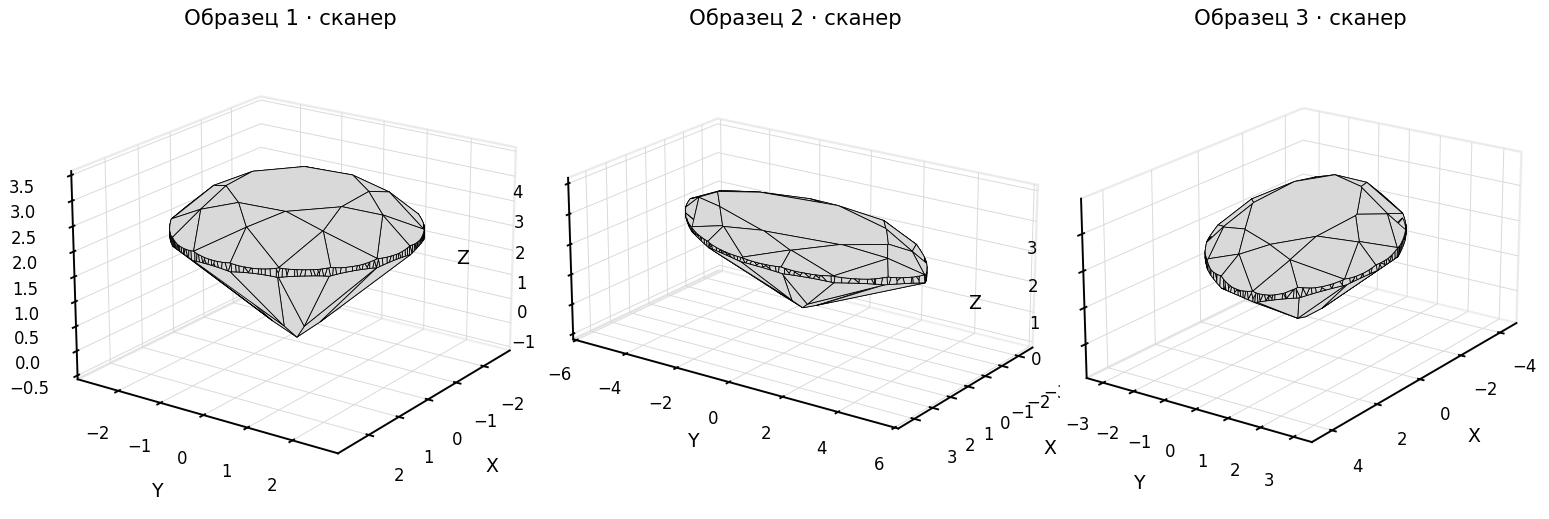
\includegraphics[width=0.95\linewidth]{fig_real_true.png}
\caption{Реальные модели сканера: образец 1, образец 2, образец 3 (короной вверх, высота нормирована)}
\label{fig:realtrue}
\end{figure}

\begin{figure}[H]
\centering
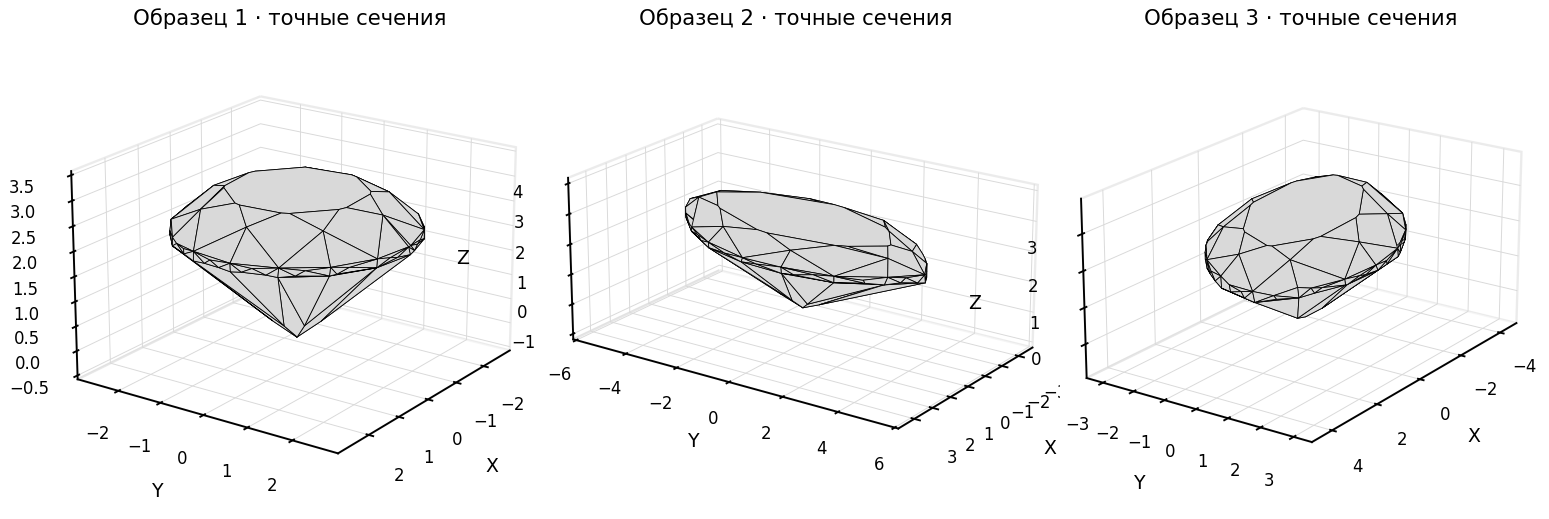
\includegraphics[width=0.95\linewidth]{fig_real_r0.png}
\caption{Восстановление по точным сечениям (пересечение полуплоскостей); показан минимальный многогранник: ошибка MSE $\le 2.3\cdot10^{-13}$}
\label{fig:realr0}
\end{figure}

\subsection{Зашумленные данные}

На реальных данных шум проявляется иначе, чем на синтетических. Зашумленные значения $R(\alpha_i)$ несовместны: не существует выпуклого тела, для которого все они были бы опорными. Поэтому пересечение полуплоскостей вырождается: при r8 остается 259--407 точек (MSE $0.32$--$0.55$), при r80 --- от 4 до 25 точек (MSE $2.17$--$5.38$), а у третьего образца восстановление вырождается полностью. Иными словами, без сглаживания обобщенное восстановление невозможно, и на реальных данных сглаживание обязательно, а не желательно.

\subsection{Сглаживание}

Сглаживание выполняется по слоям. Число гармоник увеличено до $M=32$: реальные сечения содержат десятки микро-граней (типичное значение около 30), и ряд должен их разрешать; экстремальные значения до 217 точек считаются шумом сканера.

После Фурье и МНК ошибка падает до $8.4\cdot10^{-6}$, $3.2\cdot10^{-5}$ и $2.1\cdot10^{-5}$ при r8 и до $2.9\cdot10^{-4}$, $5.5\cdot10^{-4}$ и $5.1\cdot10^{-4}$ при r80. Метод «ближайших соседей» при r8 сравним ($5.9\cdot10^{-5}$, $1.0\cdot10^{-4}$, $5.4\cdot10^{-5}$), но при r80 проигрывает на порядок: $3.1\cdot10^{-2}$, $2.7\cdot10^{-2}$ и $1.5\cdot10^{-2}$. Результаты сведены в таблице~\ref{tab:realmse} и показаны на рисунках~\ref{fig:realfft} и~\ref{fig:realuni}.

\begin{table}[H]
\centering
\caption{MSE на реальных данных (режим полуплоскостей)}
\label{tab:realmse}
\footnotesize
\begin{tabular}{|l|c|c|c|c|c|c|}
\hline
Образец & r8 & r80 & Фурье r8 & Фурье r80 & Соседи r8 & Соседи r80 \\
\hline
1 & 0.324 & 2.17 & $8.4\cdot10^{-6}$ & $2.9\cdot10^{-4}$ & $5.9\cdot10^{-5}$ & $3.1\cdot10^{-2}$ \\
2 & 0.550 & 5.38 & $3.2\cdot10^{-5}$ & $5.5\cdot10^{-4}$ & $1.0\cdot10^{-4}$ & $2.7\cdot10^{-2}$ \\
3 & 0.423 & --- & $2.1\cdot10^{-5}$ & $5.1\cdot10^{-4}$ & $5.4\cdot10^{-5}$ & $1.5\cdot10^{-2}$ \\
\hline
\end{tabular}
\end{table}

\begin{figure}[H]
\centering
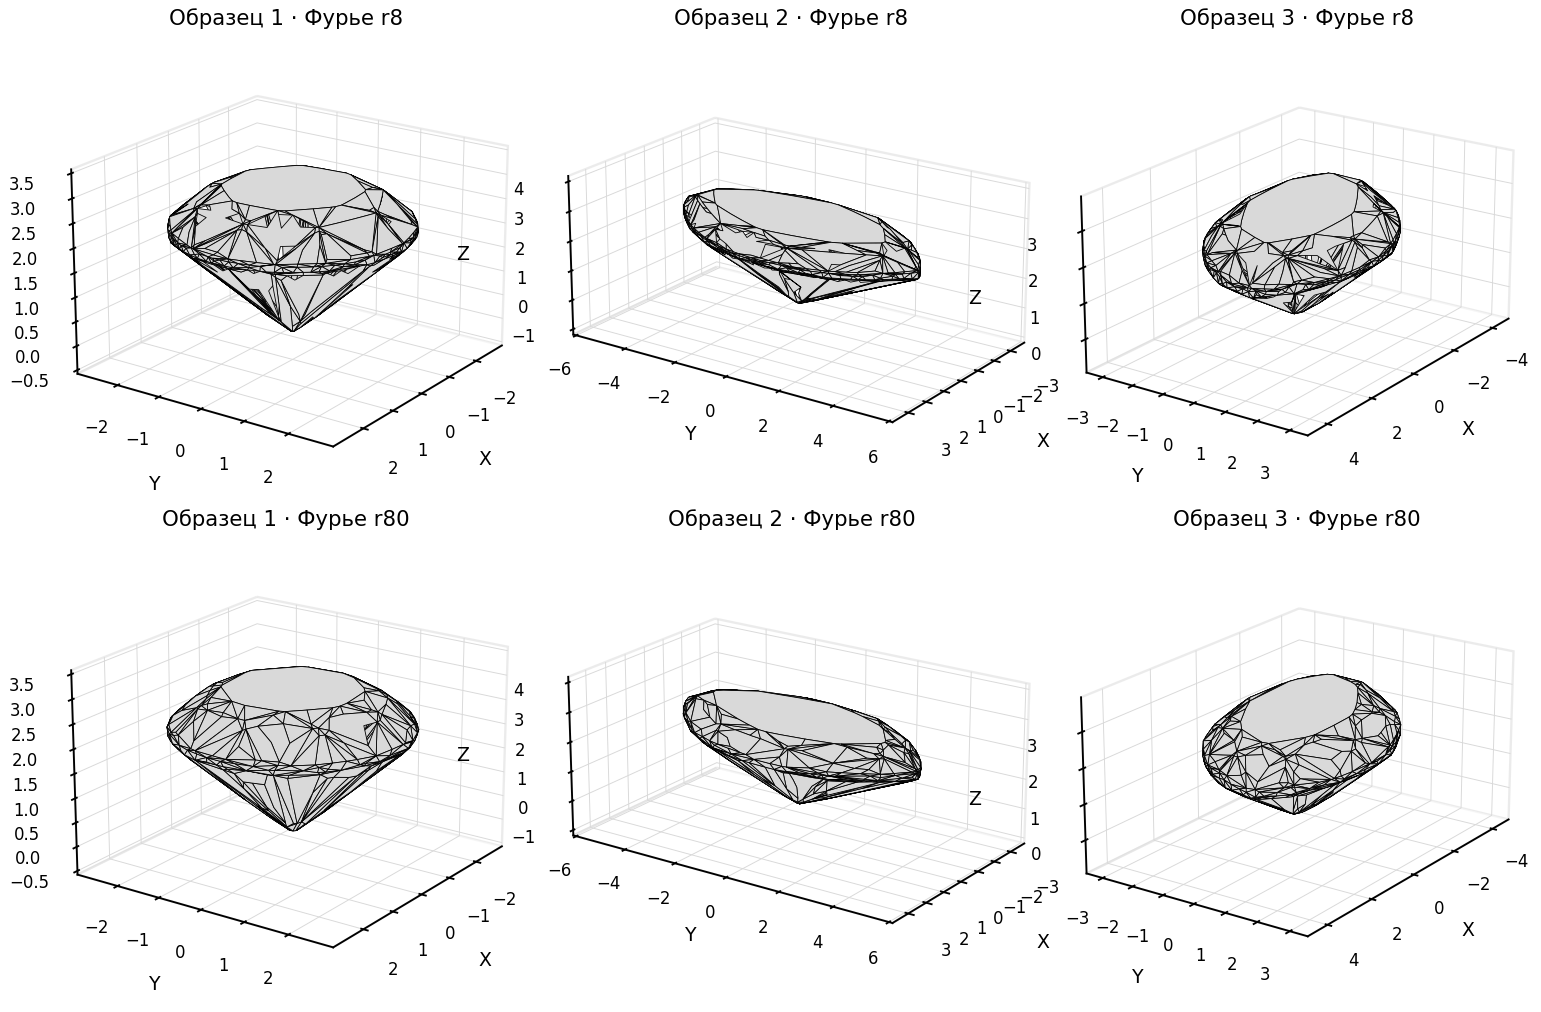
\includegraphics[width=0.9\linewidth]{fig_real_fft.png}
\caption{Реальные модели после подавления шума методом Фурье и МНК (минимальные многогранники): сверху r8, снизу r80}
\label{fig:realfft}
\end{figure}

\begin{figure}[H]
\centering
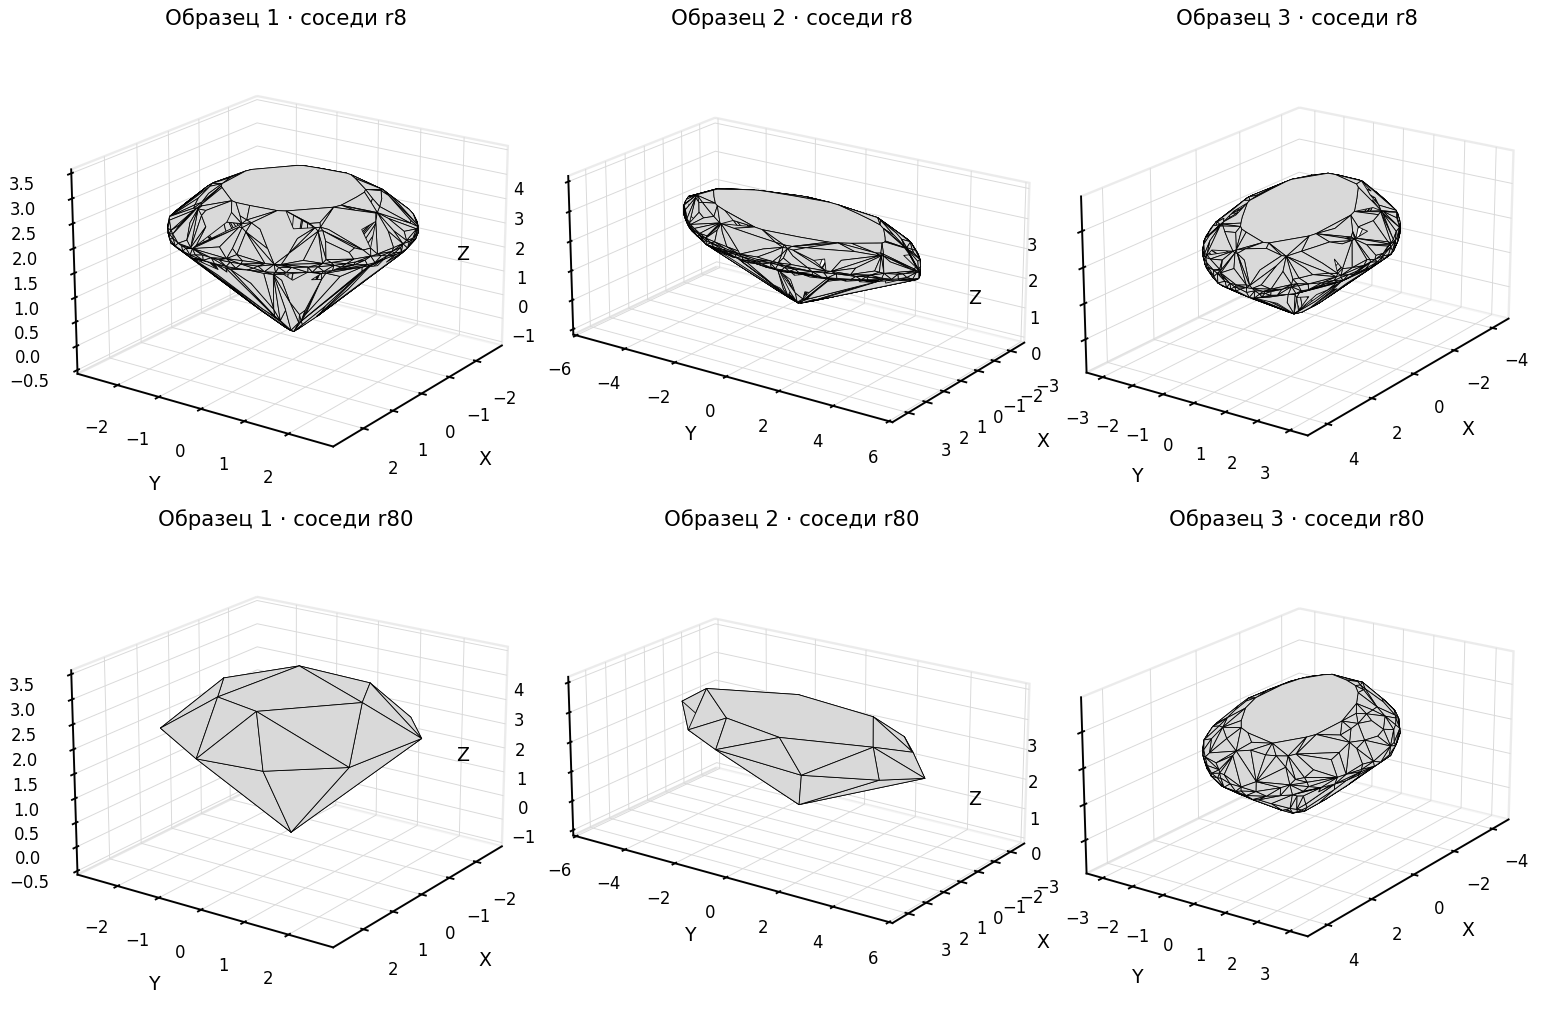
\includegraphics[width=0.9\linewidth]{fig_real_uni.png}
\caption{Реальные модели после подавления шума методом «ближайших соседей» (минимальные многогранники): сверху r8, снизу r80}
\label{fig:realuni}
\end{figure}

\subsection{Вывод по реальным данным}

Реальные данные потребовали двух изменений, которых не было видно на правильных многогранниках: восстановления через пересечение полуплоскостей и обязательного сглаживания. После этого конвейер работает: точные сечения восстанавливаются с ошибкой порядка $10^{-13}$, а зашумленные после Фурье и МНК --- с ошибкой $10^{-5}$--$10^{-4}$, то есть форма восстанавливается. Метод «ближайших соседей» при умеренном шуме сравним с МНК, но при сильном проигрывает на порядок. Результаты выгружены в OBJ (каталог $out3D\_real/obj$): точные модели и минимальные многогранники для всех вариантов.

\clearpage
\section{Программа «Огранка»}
\label{sec:app}

Для проверки метода на произвольных данных написана программа «Огранка», объединяющая весь конвейер: он принимает модель, строит сечения, добавляет шум, сглаживает, восстанавливает форму, строит минимальный многогранник и показывает результат в интерактивном окне.

Источники данных --- четыре демонстрационных тела, файлы OBJ и текстовые файлы координат $(x,y,z)$. В интерфейсе задаются несколько уровней шума одновременно (r8, r80 и произвольные), оба метода сглаживания (для «соседей» — адаптивный подбор $k_i\in[5,30]$ по зонам), режим восстановления (максимумы или полуплоскости), число слоев и направлений, автоматический минимальный многогранник с ручными параметрами --- допуском по площади и углом слияния граней.

Результат показывается в двух--шести окнах одновременно; в каждом выбирается свой вариант, выделенная грань или вершина подсвечивается во всех окнах, а камера может вращаться синхронно. Доступны режимы раскраски (однотонный, по граням, по площади), каркас, рёбра и вершины. Ниже выводятся таблица метрик (MSE, RMSE, $d_{\max}$, число вершин и граней), оценка качества (хорошо, средне, плохо) и пакетная таблица по всем загруженным моделям. Минимальный многогранник строится квадратичной декцимацией Open3D и слиянием компланарных граней, как в разделе 6.7; допуск площади и угол слияния задаются вручную. Модели выгружаются в OBJ, снимок окна --- в PNG, таблица --- в CSV.

При переносе автоматического режима в «Огранку» обнаружился артефакт, незаметный на грубых моделях. Квадратичная декцимация не сохраняет плоскости исходных фасетов: она не только удаляет вершины, но и сдвигает оставшиеся. Из-за этого плоская грань, например верхняя площадка бриллианта, распадается на несколько почти компланарных треугольников с уступом в сотые доли единицы. На экране это выглядит как скол, а площадь упрощенной модели, посчитанная до перестроения оболочки, не совпадает с площадью ее выпуклой оболочки.

Поэтому после каждой декцимации оболочка строится заново по оставшимся вершинам, а площадь для критерия $99.9\%$ считается уже по ней. Оболочка по определению дает плоские выпуклые фасеты, после чего слияние при $1^\circ$ собирает их в один многоугольник. Дополнительно вершины возвращаются на плоскости исходных фасетов, если их проекция попадает в контур грани с небольшим запасом: это убирает уступы, которые оболочка иначе сохраняет, поскольку они остаются выпуклыми. На бриллианте верхняя площадка после такой обработки становится одной четырехугольной гранью вместо двух треугольников на разных высотах. На демонстрационных телах с треугольными и пятиугольными гранями результат не меняется: октаэдр --- 6 вершин и 8 граней, икосаэдр --- 12 и 20, додекаэдр --- 20 и 12.

Программа работает локально: сервер на стандартной библиотеке Python и два пакета --- numpy и scipy; вьюпорт построен на three.js, который поставляется вместе с программой, поэтому интернет не нужен. Запуск --- python3 app.py; для macOS и Windows есть готовые ярлыки. Реальная модель (552 вершины, 60 слоев, 720 направлений, два уровня шума и оба метода сглаживания) обрабатывается примерно за 4 секунды.

\begin{figure}[H]
    \centering
    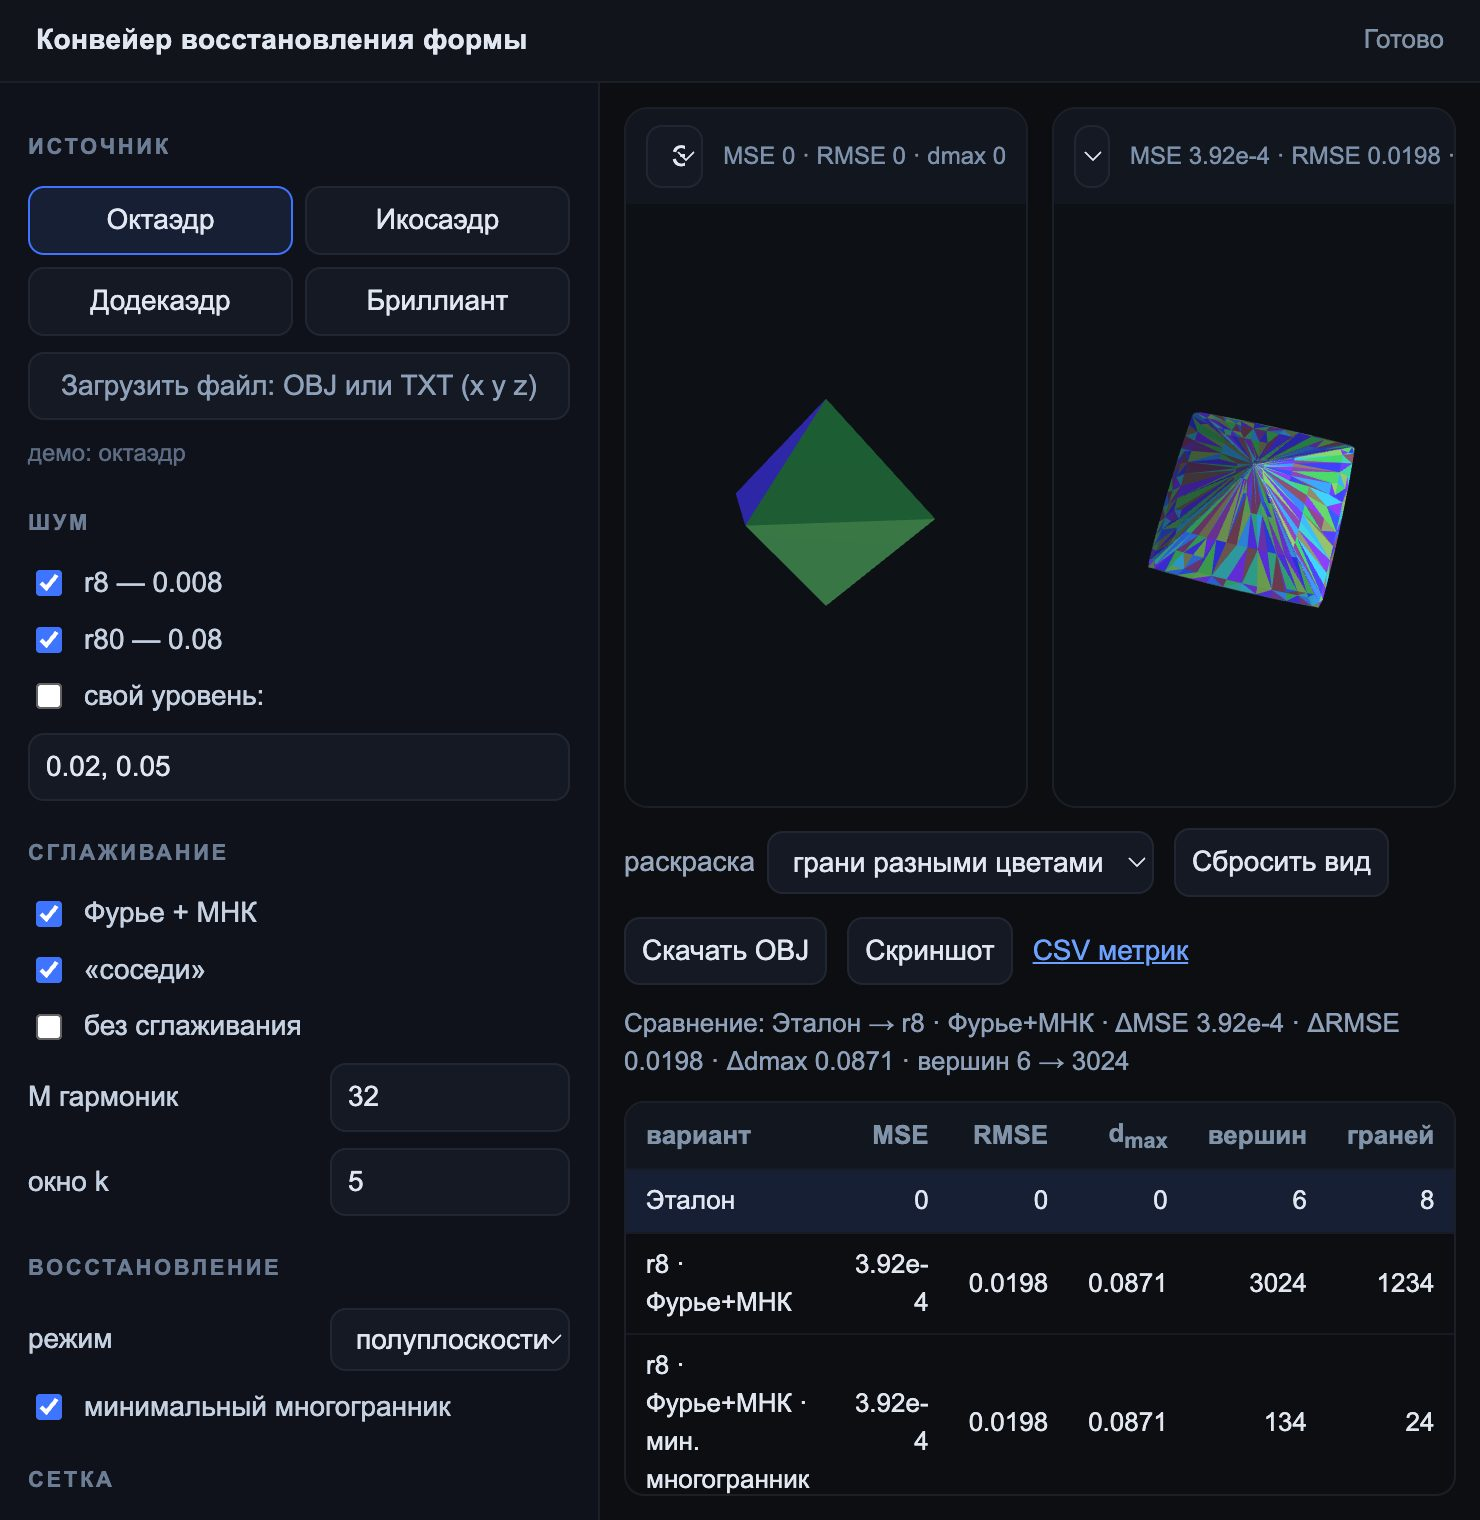
\includegraphics[width=0.8\linewidth]{app_ui.jpg}
    \caption{Окно программы: слева эталон, справа восстановленная модель; раскраска граней и метрики}
    \label{fig:app}
\end{figure}

\clearpage
\section{Вывод}

Как видно, аппроксимация методом Фурье с МНК эффективно подавляет большую дисперсию, но для умеренной дисперсии лучше подойдет метод "ближайших соседей". В трехмерном эксперименте (раздел 6) при достаточном числе гармоник преимущество МНК сохраняется и при умеренном шуме: он точнее по MSE и возвращает правильное число вершин, тогда как метод "ближайших соседей" остается полезен как более простой и в отдельных случаях дает меньшее максимальное отклонение.

\clearpage
\section{Заключение}

В работе построен и проверен конвейер восстановления формы выпуклого тела по горизонтальным точечным сечениям: по дискретной опорной функции слоя находятся вершины сечения, из вершин всех слоев собирается облако точек, по которому строится выпуклая оболочка. В 2D метод проверен на восьмиугольнике, в 3D --- на четырех телах с переменным сечением: октаэдре, икосаэдре, додекаэдре и бриллианте короной вверх. Для каждого тела сгенерировано 60 сечений с шагом $0.05$ по высоте и 720 направлений с шагом $0.5^\circ$; шум добавлялся с амплитудами $r_v=0.008$ (r8) и $r_v=0.08$ (r80).

На точных данных эталон восстанавливается практически точно: средняя квадратичная ошибка не превышает $9.4\cdot10^{-7}$, а отличие от аналитических сечений --- только ошибка дискретизации по углу. Без подавления шума число восстановленных вершин вырастает с 240--600 до 12--14 тысяч: каждый шумовой всплеск становится локальным максимумом, оболочка покрывается мелкими гранями, а MSE достигает $0.0136$.

Оба метода сглаживания возвращают форму. Аппроксимация рядом Фурье с МНК снижает MSE в 7--266 раз и дает 247--600 вершин --- практически столько же, сколько у эталона. Метод «ближайших соседей» снижает MSE в 3--13 раз, но оставляет 871--3787 вершин: часть ложных максимумов сохраняется. По интегральной ошибке МНК точнее в 1.3--40 раз; лишь на икосаэдре при r8 метод соседей дает меньшее максимальное отклонение ($0.089$ против $0.105$), потому что МНК сильнее сглаживает и «срезает» острые углы.

Отдельный методический результат --- выбор числа гармоник. Ряд должен разрешать не только вершины, но и углы сечения: при $M=8$ на десятиугольных сечениях икосаэдра ошибка при r80 составила $0.00180$, а при $M=12$ --- $0.00077$. Для додекаэдра, где сечение содержит не более шести вершин, увеличение $M$ почти не меняет результат ($0.00104$ и $0.00099$). Правило «$M$ не меньше максимального числа вершин сечения» объясняет и разницу между 2D- и 3D-выводами: в 2D при восьмивершинном сечении $M=8$ было достаточно, и при умеренном шуме выигрывали соседи; в 3D при достаточном $M$ преимущество МНК сохраняется и при умеренном шуме.

Ограничения метода: он работает для выпуклых тел, чувствителен к выбору числа гармоник и к сильному шуму на малых сечениях (у колета бриллианта относительный вклад шума максимален), а при сильном шуме оставляет ложные вершины. Порог погрешности зависит от геометрической сложности и детализации фигуры.

Наконец, наблюдение, которое стоит за всеми числами: человек и компьютер видят одну и ту же задачу по-разному. Даже если задача поставлена корректно и кажется человеку тривиальной, компьютер может подменять концепции и выполнить то, что по условию не требовалось, либо иначе исказить результат из-за накапливаемых вычислительных погрешностей и отсутствия человеческого опыта. Компьютер может решать одну и ту же задачу несколькими способами, которые человеку кажутся логически абсурдными, --- отсюда ошибки и неопределенности: «не увидеть» лишнюю грань, добавить ее или построить многогранник по облаку точек по-разному. Чем сложнее геометрическая форма, тем сложнее, хитрее и продуманнее требуются алгоритмы. Возможно, будущее --- за нейросетевыми алгоритмами.

\newpage
\clearpage
\phantomsection
\renewcommand{\refname}{Список литературы}
\addcontentsline{toc}{section}{Список литературы}
\begin{thebibliography}{99}\sloppy

\bibitem{tomography}
Kak A., Slaney M.
Principles of Computerized Tomographic Imaging.
\url{http://www.slaney.org/pct/pct-toc.html}

\bibitem{shape}
Szeliski R.
Computer Vision: Algorithms and Applications.
Разделы, посвящённые восстановлению формы и силуэтам.
\url{https://szeliski.org/Book/}

\bibitem{visualhull}
Laurentini A.
The Visual Hull Concept for Silhouette-Based Image Understanding //
IEEE Transactions on Pattern Analysis and Machine Intelligence.
\url{https://ieeexplore.ieee.org/document/273735}

\bibitem{cgal}
CGAL Computational Geometry Library.
Материалы по выпуклым оболочкам и вычислительной геометрии.
\url{https://www.cgal.org/}

\bibitem{habr-convexhull}
Григорьев~А.
Выпуклая оболочка: алгоритмы построения и анализ.
\url{https://habr.com/ru/post/144921/}

\bibitem{sidorenko}
Сидоренко~А.А., Меженин~А.В.
Обработка облаков точек для повышения качества 3D-моделей.
\url{https://kmu.itmo.ru/digests/article/14050}

\bibitem{churilin}
Чурилин~О.И., Белов~Ю.С.
Методы устранения артефактов и шумов при цифровой 3D-реконструкции объектов из изображений.
\url{https://library.bmstu.ru/Catalog/Details/596871}

\bibitem{artemiev}
Артемьев~В.М., Наумов~А.О., Кохан~Л.Л.
Адаптивная фильтрация комплексированных измерений методом наименьших квадратов.
\url{http://depositary.belisa.org.by/EDNI/Periodicals/Articles/Details.aspx?Key_Journal=32&Id=965}

\bibitem{golikov}
Голиков~Р.Ю., Коростелкина~И.А., Ляпина~И.Р., Мекшенева~Ж.В.
Восстановление формы сильно зашумленного сигнала на основе интегро-дифференциального преобразования и аппроксимации интегральной кривой.
\url{http://www.appliedinformatics.ru/r/free/article/index.php?article_id_4=3189}

\bibitem{habr-graph-laplacian}
Удаление шума и деформация 3D-облаков точек в Python с помощью графовых лапласианов.
\url{https://habr.com/ru/articles/1010452/}

\end{thebibliography}

\end{document}